\documentclass[10pt,a4paper]{article}
\usepackage[utf8]{inputenc}
\usepackage{fullpage}
% \usepackage[margin=0.1cm]{geometry}

\usepackage[dvipsnames]{xcolor}
\usepackage{amsmath}
\usepackage{amssymb}
\usepackage{amsfonts}
\usepackage{amsthm}
\usepackage{graphicx}
\usepackage{tikz}
\usepackage{tikz-cd}
\usetikzlibrary{calc}
\usepackage{amscd}


\newtheorem{definition}{Definition}[section]
\newtheorem{theorem}{Theorem}[section]
\newtheorem{lemma}[theorem]{Lemma}
\newtheorem{remark}[theorem]{Remark}
\newtheorem{example}[theorem]{Example}
\newtheorem{proposition}[theorem]{Proposition}

\makeatletter
\newcommand\suchthat{%
 \@ifstar
  {\mathrel{}\middle|\mathrel{}}
  {\mid}%
}
\makeatother

\newcommand{\Ceins}[1]{C_{1,#1}}
\newcommand{\Czwei}[1]{C_{2,#1}}
\newcommand{\Cdrei}[1]{C_{3,#1}}
\newcommand{\Cvier}[2]{C_{4,#1,#2}}
\newcommand{\Cfive}[2]{C_{5,#1,#2}}
% \newcommand{\Ceins}{\sqrt{n}}
% \newcommand{\Czwei}{\sqrt{2n}}



\newcommand{\Perm}{{\operatorname{Perm}}}

\newcommand{\linhull}{{\operatorname{span}}}
\newcommand{\convexhull}{{\operatorname{convex}}}

\newcommand{\Poinc}{\frakP}
\newcommand{\Bogov}{\frakB}

\newcommand{\mollifier}{\frakm}

\newcommand{\eps}{\epsilon}

\newcommand{\Id}{\rm{Id}}

\newcommand{\Lip}{\rm{Lip}}

\newcommand{\diff}{\mathop{}\!\mathrm{d}}

\DeclareMathOperator{\adj}{adj}
%\newcommand{\adj}{{\rm adj}}
\newcommand{\inv}{{-1}}
\newcommand{\invt}{{-t}}
\newcommand{\tinv}{{-t}}
\newcommand{\determinant}{{\operatorname{det}}}
\DeclareMathOperator{\Jacobian}{{\rm Jac}}
% \newcommand{\Jacobian}{{\rm Jac}}
\newcommand{\dimension}{\operatorname{dim}}
\newcommand{\sgn}{\operatorname{sgn}}
\newcommand{\adjugate}{\operatorname{adj}}
\newcommand{\sym}{\operatorname{sym}}
\newcommand{\signum}{\operatorname{sgn}}
\newcommand{\kronecker}{{\hat\delta}}
\newcommand{\dom}{\operatorname{dom}}
\newcommand{\codom}{\operatorname{codom}}
\newcommand{\rng}{\operatorname{ran}}
\newcommand{\convex}{\operatorname{convex}}
\newcommand{\coker}{\operatorname{coker}}
\newcommand{\coran}{\operatorname{coran}}

\newcommand{\dif}{{\mathrm d}}
\newcommand{\Dif}{{\mathrm D}}
\newcommand{\grad}{\operatorname{grad}}
\newcommand{\Grad}{\operatorname{Grad}}
\newcommand{\curl}{\operatorname{curl}}
\newcommand{\Curl}{\operatorname{Curl}}
\newcommand{\rot}{\curl}
\newcommand{\divergence}{\operatorname{div}}
\newcommand{\diver}{\operatorname{div}}
\newcommand{\svcurl}{\operatorname{sv-curl}}
\newcommand{\vscurl}{\operatorname{vs-curl}}
\newcommand{\sdiver}{\operatorname{sdiv}}
\newcommand{\Sdiver}{\operatorname{Sdiv}}
\newcommand{\sgrad}{\operatorname{sgrad}}
\newcommand{\Sgrad}{\operatorname{Sgrad}}
\newcommand{\Laplace}{\bigtriangleup}
\newcommand{\laplace}{\bigtriangleup}
\newcommand{\laplacian}{\laplace}
\newcommand{\Laplacian}{\laplace}
% \newcommand{\cartan}{{\mathsf d}}
% \newcommand{\cartanx}{{\mathsf d}x}
\newcommand{\cartan}{d}
\newcommand{\cartanx}{dx}

%\newcommand{\argmin}{\operatorname{argmin}}
\DeclareMathOperator*{\argmin}{{\rm argmin}}

% \DeclareMathOperator*{\carapace}{{\rm corona}}
\DeclareMathOperator*{\carapace}{{\partial \rm st}}

\newcommand{\supp}{\operatorname{supp}}
\newcommand{\esssup}{{\operatorname{esssup}}}
\newcommand{\essinf}{{\operatorname{essinf}}}

\newcommand{\equivalent}{ \Longleftrightarrow }
\newcommand{\vol}{\operatorname{vol}}
\newcommand{\st}{ \mid }
\newcommand{\diam}{{\operatorname{diam}}}
\newcommand{\height}{\operatorname{height}}
\newcommand{\dist}{\operatorname{dist}}
\newcommand{\patch}{\operatorname{st}}

\newcommand{\Trace}{\operatorname{Tr}}
\newcommand{\Tr}{\operatorname{Tr}}
\newcommand{\trace}{\operatorname{tr}}
\newcommand{\normaltrace}{\operatorname{nm}}
\newcommand{\tr}{\operatorname{tr}}
\newcommand{\Ext}{\operatorname{Ext}}
\newcommand{\Ex}{\operatorname{Ex}}
\newcommand{\ext}{\operatorname{ext}}

\newcommand{\Poincare}{\sfP}
\newcommand*{\volsphere}[1]{\color{red}{S_{#1}}}
\newcommand*{\volball}[1]{B_{#1}}

\newcommand{\subsimplex}{\calS^{\downarrow}}
\newcommand{\supsimplex}{\calS^{\uparrow}}
\newcommand{\supersimplex}{\supsimplex}
\newcommand{\orientation}{\mathscr{O}}
\newcommand{\restrict}{R}

\newcommand{\Mesh}{\calT}
\newcommand{\Vertices}{\calV}
\newcommand{\Edges}{\calE}
\newcommand{\Faces}{\calF}
\newcommand{\Ball}{\calB}
\newcommand{\Sphere}{S}
\newcommand{\underlying}[1]{\left| #1 \right|}

\newcommand{\Distr}{\calD}
\newcommand{\Cont}{\calC}
\newcommand{\Lebesgue}{L}
\newcommand{\Sobolev}{W}
\newcommand{\SOBOLEV}{\bfW}
\newcommand{\SobolevLambda}{W\Lambda}
\newcommand{\Alt}{\Lambda}
\newcommand{\loc}{\rm{loc}}

\newcommand{\Ned}{{\calN d}}
\newcommand{\RT}{{\calR T}}
\newcommand{\BDM}{{\calB \calD \calM}}
  

\newcommand*{\ConstantPF}{C_{\rm{PF}}}







\newcommand{\bbA}{{\mathbb A}}
\newcommand{\bbB}{{\mathbb B}}
\newcommand{\bbC}{{\mathbb C}}
\newcommand{\bbD}{{\mathbb D}}
\newcommand{\bbE}{{\mathbb E}}
\newcommand{\bbF}{{\mathbb F}}
\newcommand{\bbG}{{\mathbb G}}
\newcommand{\bbH}{{\mathbb H}}
\newcommand{\bbI}{{\mathbb I}}
\newcommand{\bbJ}{{\mathbb J}}
\newcommand{\bbK}{{\mathbb K}}
\newcommand{\bbL}{{\mathbb L}}
\newcommand{\bbM}{{\mathbb M}}
\newcommand{\bbN}{{\mathbb N}}
\newcommand{\bbO}{{\mathbb O}}
\newcommand{\bbP}{{\mathbb P}}
\newcommand{\bbQ}{{\mathbb Q}}
\newcommand{\bbR}{{\mathbb R}}
\newcommand{\bbS}{{\mathbb S}}
\newcommand{\bbT}{{\mathbb T}}
\newcommand{\bbU}{{\mathbb U}}
\newcommand{\bbV}{{\mathbb V}}
\newcommand{\bbW}{{\mathbb W}}
\newcommand{\bbX}{{\mathbb X}}
\newcommand{\bbY}{{\mathbb Y}}
\newcommand{\bbZ}{{\mathbb Z}}

\newcommand{\bfA}{{\mathbf A}}
\newcommand{\bfB}{{\mathbf B}}
\newcommand{\bfC}{{\mathbf C}}
\newcommand{\bfD}{{\mathbf D}}
\newcommand{\bfE}{{\mathbf E}}
\newcommand{\bfF}{{\mathbf F}}
\newcommand{\bfG}{{\mathbf G}}
\newcommand{\bfH}{{\mathbf H}}
\newcommand{\bfI}{{\mathbf I}}
\newcommand{\bfJ}{{\mathbf J}}
\newcommand{\bfK}{{\mathbf K}}
\newcommand{\bfL}{{\mathbf L}}
\newcommand{\bfM}{{\mathbf M}}
\newcommand{\bfN}{{\mathbf N}}
\newcommand{\bfO}{{\mathbf O}}
\newcommand{\bfP}{{\mathbf P}}
\newcommand{\bfQ}{{\mathbf Q}}
\newcommand{\bfR}{{\mathbf R}}
\newcommand{\bfS}{{\mathbf S}}
\newcommand{\bfT}{{\mathbf T}}
\newcommand{\bfU}{{\mathbf U}}
\newcommand{\bfV}{{\mathbf V}}
\newcommand{\bfW}{{\mathbf W}}
\newcommand{\bfX}{{\mathbf X}}
\newcommand{\bfY}{{\mathbf Y}}
\newcommand{\bfZ}{{\mathbf Z}}

\newcommand{\bfa}{{\mathbf a}}
\newcommand{\bfb}{{\mathbf b}}
\newcommand{\bfc}{{\mathbf c}}
\newcommand{\bfd}{{\mathbf d}}
\newcommand{\bfe}{{\mathbf e}}
\newcommand{\bff}{{\mathbf f}}
\newcommand{\bfg}{{\mathbf g}}
\newcommand{\bfh}{{\mathbf h}}
\newcommand{\bfi}{{\mathbf i}}
\newcommand{\bfj}{{\mathbf j}}
\newcommand{\bfk}{{\mathbf k}}
\newcommand{\bfl}{{\mathbf l}}
\newcommand{\bfm}{{\mathbf m}}
\newcommand{\bfn}{{\mathbf n}}
\newcommand{\bfo}{{\mathbf o}}
\newcommand{\bfp}{{\mathbf p}}
\newcommand{\bfq}{{\mathbf q}}
\newcommand{\bfr}{{\mathbf r}}
\newcommand{\bfs}{{\mathbf s}}
\newcommand{\bft}{{\mathbf t}}
\newcommand{\bfu}{{\mathbf u}}
\newcommand{\bfv}{{\mathbf v}}
\newcommand{\bfw}{{\mathbf w}}
\newcommand{\bfx}{{\mathbf x}}
\newcommand{\bfy}{{\mathbf y}}
\newcommand{\bfz}{{\mathbf z}}


\newcommand{\calA}{{\mathcal A}}
\newcommand{\calB}{{\mathcal B}}
\newcommand{\calC}{{\mathcal C}}
\newcommand{\calD}{{\mathcal D}}
\newcommand{\calE}{{\mathcal E}}
\newcommand{\calF}{{\mathcal F}}
\newcommand{\calG}{{\mathcal G}}
\newcommand{\calH}{{\mathcal H}}
\newcommand{\calI}{{\mathcal I}}
\newcommand{\calJ}{{\mathcal J}}
\newcommand{\calK}{{\mathcal K}}
\newcommand{\calL}{{\mathcal L}}
\newcommand{\calM}{{\mathcal M}}
\newcommand{\calN}{{\mathcal N}}
\newcommand{\calO}{{\mathcal O}}
\newcommand{\calP}{{\mathcal P}}
\newcommand{\calQ}{{\mathcal Q}}
\newcommand{\calR}{{\mathcal R}}
\newcommand{\calS}{{\mathcal S}}
\newcommand{\calT}{{\mathcal T}}
\newcommand{\calU}{{\mathcal U}}
\newcommand{\calV}{{\mathcal V}}
\newcommand{\calW}{{\mathcal W}}
\newcommand{\calX}{{\mathcal X}}
\newcommand{\calY}{{\mathcal Y}}
\newcommand{\calZ}{{\mathcal Z}}

\newcommand{\fraka}{{\mathfrak a}}
\newcommand{\frakb}{{\mathfrak b}}
\newcommand{\frakc}{{\mathfrak c}}
\newcommand{\frakd}{{\mathfrak d}}
\newcommand{\frake}{{\mathfrak e}}
\newcommand{\frakf}{{\mathfrak f}}
\newcommand{\frakg}{{\mathfrak g}}
\newcommand{\frakh}{{\mathfrak h}}
\newcommand{\fraki}{{\mathfrak i}}
\newcommand{\frakj}{{\mathfrak j}}
\newcommand{\frakk}{{\mathfrak k}}
\newcommand{\frakl}{{\mathfrak l}}
\newcommand{\frakm}{{\mathfrak m}}
\newcommand{\frakn}{{\mathfrak n}}
\newcommand{\frako}{{\mathfrak o}}
\newcommand{\frakp}{{\mathfrak p}}
\newcommand{\frakq}{{\mathfrak q}}
\newcommand{\frakr}{{\mathfrak r}}
\newcommand{\fraks}{{\mathfrak s}}
\newcommand{\frakt}{{\mathfrak t}}
\newcommand{\fraku}{{\mathfrak u}}
\newcommand{\frakv}{{\mathfrak v}}
\newcommand{\frakw}{{\mathfrak w}}
\newcommand{\frakx}{{\mathfrak x}}
\newcommand{\fraky}{{\mathfrak y}}
\newcommand{\frakz}{{\mathfrak z}}
\newcommand{\frakA}{{\mathfrak A}}
\newcommand{\frakB}{{\mathfrak B}}
\newcommand{\frakC}{{\mathfrak C}}
\newcommand{\frakD}{{\mathfrak D}}
\newcommand{\frakE}{{\mathfrak E}}
\newcommand{\frakF}{{\mathfrak F}}
\newcommand{\frakG}{{\mathfrak G}}
\newcommand{\frakH}{{\mathfrak H}}
\newcommand{\frakI}{{\mathfrak I}}
\newcommand{\frakJ}{{\mathfrak J}}
\newcommand{\frakK}{{\mathfrak K}}
\newcommand{\frakL}{{\mathfrak L}}
\newcommand{\frakM}{{\mathfrak M}}
\newcommand{\frakN}{{\mathfrak N}}
\newcommand{\frakO}{{\mathfrak O}}
\newcommand{\frakP}{{\mathfrak P}}
\newcommand{\frakQ}{{\mathfrak Q}}
\newcommand{\frakR}{{\mathfrak R}}
\newcommand{\frakS}{{\mathfrak S}}
\newcommand{\frakT}{{\mathfrak T}}
\newcommand{\frakU}{{\mathfrak U}}
\newcommand{\frakV}{{\mathfrak V}}
\newcommand{\frakW}{{\mathfrak W}}
\newcommand{\frakX}{{\mathfrak X}}
\newcommand{\frakY}{{\mathfrak Y}}
\newcommand{\frakZ}{{\mathfrak Z}}







\newcommand{\rma}{{\mathrm a}}
\newcommand{\rmb}{{\mathrm b}}
\newcommand{\rmc}{{\mathrm c}}
\newcommand{\rmd}{{\mathrm d}}
\newcommand{\rme}{{\mathrm e}}
\newcommand{\rmf}{{\mathrm f}}
\newcommand{\rmg}{{\mathrm g}}
\newcommand{\rmh}{{\mathrm h}}
\newcommand{\rmi}{{\mathrm i}}
\newcommand{\rmj}{{\mathrm j}}
\newcommand{\rmk}{{\mathrm k}}
\newcommand{\rml}{{\mathrm l}}
\newcommand{\rmm}{{\mathrm m}}
\newcommand{\rmn}{{\mathrm n}}
\newcommand{\rmo}{{\mathrm o}}
\newcommand{\rmp}{{\mathrm p}}
\newcommand{\rmq}{{\mathrm q}}
\newcommand{\rmr}{{\mathrm r}}
\newcommand{\rms}{{\mathrm s}}
\newcommand{\rmt}{{\mathrm t}}
\newcommand{\rmu}{{\mathrm u}}
\newcommand{\rmv}{{\mathrm v}}
\newcommand{\rmw}{{\mathrm w}}
\newcommand{\rmx}{{\mathrm x}}
\newcommand{\rmy}{{\mathrm y}}
\newcommand{\rmz}{{\mathrm z}}
\newcommand{\rmA}{{\mathrm A}}
\newcommand{\rmB}{{\mathrm B}}
\newcommand{\rmC}{{\mathrm C}}
\newcommand{\rmD}{{\mathrm D}}
\newcommand{\rmE}{{\mathrm E}}
\newcommand{\rmF}{{\mathrm F}}
\newcommand{\rmG}{{\mathrm G}}
\newcommand{\rmH}{{\mathrm H}}
\newcommand{\rmI}{{\mathrm I}}
\newcommand{\rmJ}{{\mathrm J}}
\newcommand{\rmK}{{\mathrm K}}
\newcommand{\rmL}{{\mathrm L}}
\newcommand{\rmM}{{\mathrm M}}
\newcommand{\rmN}{{\mathrm N}}
\newcommand{\rmO}{{\mathrm O}}
\newcommand{\rmP}{{\mathrm P}}
\newcommand{\rmQ}{{\mathrm Q}}
\newcommand{\rmR}{{\mathrm R}}
\newcommand{\rmS}{{\mathrm S}}
\newcommand{\rmT}{{\mathrm T}}
\newcommand{\rmU}{{\mathrm U}}
\newcommand{\rmV}{{\mathrm V}}
\newcommand{\rmW}{{\mathrm W}}
\newcommand{\rmX}{{\mathrm X}}
\newcommand{\rmY}{{\mathrm Y}}
\newcommand{\rmZ}{{\mathrm Z}}





\newcommand{\scrA}{{\mathscr A}}
\newcommand{\scrB}{{\mathscr B}}
\newcommand{\scrC}{{\mathscr C}}
\newcommand{\scrD}{{\mathscr D}}
\newcommand{\scrE}{{\mathscr E}}
\newcommand{\scrF}{{\mathscr F}}
\newcommand{\scrG}{{\mathscr G}}
\newcommand{\scrH}{{\mathscr H}}
\newcommand{\scrI}{{\mathscr I}}
\newcommand{\scrJ}{{\mathscr J}}
\newcommand{\scrK}{{\mathscr K}}
\newcommand{\scrL}{{\mathscr L}}
\newcommand{\scrM}{{\mathscr M}}
\newcommand{\scrN}{{\mathscr N}}
\newcommand{\scrO}{{\mathscr O}}
\newcommand{\scrP}{{\mathscr P}}
\newcommand{\scrQ}{{\mathscr Q}}
\newcommand{\scrR}{{\mathscr R}}
\newcommand{\scrS}{{\mathscr S}}
\newcommand{\scrT}{{\mathscr T}}
\newcommand{\scrU}{{\mathscr U}}
\newcommand{\scrV}{{\mathscr V}}
\newcommand{\scrW}{{\mathscr W}}
\newcommand{\scrX}{{\mathscr X}}
\newcommand{\scrY}{{\mathscr Y}}
\newcommand{\scrZ}{{\mathscr Z}}


\newcommand{\veca}{{\vec a}}
\newcommand{\vecb}{{\vec b}}
\newcommand{\vecc}{{\vec c}}
\newcommand{\vecd}{{\vec d}}
\newcommand{\vece}{{\vec e}}
\newcommand{\vecf}{{\vec f}}
\newcommand{\vecg}{{\vec g}}
\newcommand{\vech}{{\vec h}}
\newcommand{\veci}{{\vec i}}
\newcommand{\vecj}{{\vec j}}
\newcommand{\veck}{{\vec k}}
\newcommand{\vecl}{{\vec l}}
\newcommand{\vecm}{{\vec m}}
\newcommand{\vecn}{{\vec n}}
\newcommand{\veco}{{\vec o}}
\newcommand{\vecp}{{\vec p}}
\newcommand{\vecq}{{\vec q}}
\newcommand{\vecr}{{\vec r}}
\newcommand{\vecs}{{\vec s}}
\newcommand{\vect}{{\vec t}}
\newcommand{\vecu}{{\vec u}}
\newcommand{\vecv}{{\vec v}}
\newcommand{\vecw}{{\vec w}}
\newcommand{\vecx}{{\vec x}}
\newcommand{\vecy}{{\vec y}}
\newcommand{\vecz}{{\vec z}}
\newcommand{\vecA}{{\vec A}}
\newcommand{\vecB}{{\vec B}}
\newcommand{\vecC}{{\vec C}}
\newcommand{\vecD}{{\vec D}}
\newcommand{\vecE}{{\vec E}}
\newcommand{\vecF}{{\vec F}}
\newcommand{\vecG}{{\vec G}}
\newcommand{\vecH}{{\vec H}}
\newcommand{\vecI}{{\vec I}}
\newcommand{\vecJ}{{\vec J}}
\newcommand{\vecK}{{\vec K}}
\newcommand{\vecL}{{\vec L}}
\newcommand{\vecM}{{\vec M}}
\newcommand{\vecN}{{\vec N}}
\newcommand{\vecO}{{\vec O}}
\newcommand{\vecP}{{\vec P}}
\newcommand{\vecQ}{{\vec Q}}
\newcommand{\vecR}{{\vec R}}
\newcommand{\vecS}{{\vec S}}
\newcommand{\vecT}{{\vec T}}
\newcommand{\vecU}{{\vec U}}
\newcommand{\vecV}{{\vec V}}
\newcommand{\vecW}{{\vec W}}
\newcommand{\vecX}{{\vec X}}
\newcommand{\vecY}{{\vec Y}}
\newcommand{\vecZ}{{\vec Z}}


\newcommand{\boldalpha}{{\boldsymbol\alpha}}
\newcommand{\boldbeta}{{\boldsymbol\beta}}
\newcommand{\boldgamma}{{\boldsymbol\gamma}}
\newcommand{\bolddelta}{{\boldsymbol\delta}}
\newcommand{\boldepsilon}{{\boldsymbol\epsilon}}
\newcommand{\boldzeta}{{\boldsymbol\zeta}}
\newcommand{\boldeta}{{\boldsymbol\eta}}
\newcommand{\boldtheta}{{\boldsymbol\theta}}
\newcommand{\boldiota}{{\boldsymbol\iota}}
\newcommand{\boldkappa}{{\boldsymbol\kappa}}
\newcommand{\boldlambda}{{\boldsymbol\lambda}}
\newcommand{\boldmu}{{\boldsymbol\mu}}
\newcommand{\boldnu}{{\boldsymbol\nu}}
\newcommand{\boldxi}{{\boldsymbol\xi}}
\newcommand{\boldomicron}{{\boldsymbol o}}
\newcommand{\boldpi}{{\boldsymbol\pi}}
\newcommand{\boldrho}{{\boldsymbol\rho}}
\newcommand{\boldsigma}{{\boldsymbol\sigma}}
\newcommand{\boldtau}{{\boldsymbol\tau}}
\newcommand{\boldupsilon}{{\boldsymbol\upsilon}}
\newcommand{\boldphi}{{\boldsymbol\phi}}
\newcommand{\boldchi}{{\boldsymbol\chi}}
\newcommand{\boldpsi}{{\boldsymbol\psi}}
\newcommand{\boldomega}{{\boldsymbol\omega}}



\usepackage{xcolor}          % 
\usepackage{comment}          % 
\usepackage[colorlinks=true]{hyperref}         % For hypertext links
% Make the hyperlinks look similar to arXiv's
\hypersetup{
    colorlinks=true,
    linkcolor=Maroon,    % Color of internal links (sections)
    citecolor=red,    % Color of citations
    urlcolor=blue,     % Color for URLs
    urlbordercolor={1 1 1},
    pdfborder={0.5 0.5 0}  % Removes the border around the links
}
\usepackage{tikz-3dplot}      % 3d plots 
\usepackage{enumitem}
\setitemize[1]{left=0.0cm} 


% Added by MV 
\usepackage{bm} % preferred version of bold symbols
\usepackage[normalem]{ulem} % for strikethrough (\sout) in collaborative writing
% \usepackage{cancel} % for strikethrough in collaborative writing (math formulas)
% \usepackage[textsize=tiny,color=blue!10!white]{todonotes}
% \newcommand{\todo}[1]{{\colorbox{yellow}{#1}}}
\setlength{\marginparwidth}{2cm}
    
\newcommand\cye[1]{%
\protect\leavevmode
\begingroup
    \color{blue}%
    #1%
\endgroup
}
% \color{red!35!yellow}

\newcommand{\mwl}[1]{{\color{red}#1}}
\newcommand{\notice}[1]{{\color{red}REMARK: #1}}
\newcommand{\disk}{\cye{ball}}
\newcommand{\todo}[1]{{\color{RedOrange}\textbf{#1}}}








% LTeX: enabled=false
% Title, authors, and affiliations
% \title{Poincar\'e--Friedrichs constants over domains with shellable triangulations}
% \author{Th\'eophile Chaumont-Frelet, Martin Werner Licht, Martin Vohral\'ik}

\title{Computable Poincar\'e--Friedrichs constants for the $L^{p}$ de~Rham complex over convex domains and domains with shellable triangulations}
\author{
    Th\'eophile Chaumont-Frelet\thanks{Inria Univ. Lille and Laboratoire Paul Painlev\'e, 59655 Villeneuve-d'Ascq, France, \texttt{theophile.chaumont@inria.fr}} \and
    Martin Werner Licht\thanks{\'Ecole Polytechnique F\'ed\'erale de Lausanne, CH-1015 Lausanne, Switzerland, \texttt{martin.licht@epfl.ch}} \and
    Martin Vohral\'ik\thanks{Inria, 48 rue Barrault, 75647 Paris, France \& CERMICS, Ecole des Ponts, 77455 Marne-la-Vall\'ee, France, \texttt{martin.vohralik@inria.fr}}
}
\date{}
% LTeX: enabled=true


\begin{document}

\tableofcontents



\section{Original 2D table}



\begin{table}[t]
    \centering
    \begin{tabular}{|c|c|c|c|c|c|c|c|c|}
        \hline
                        & $\grad$ ref  & $\grad$ est & $\grad$ ratio      & $\grad$ est & $\grad$ ratio      & $\divergence$ ref  & $\divergence$ est  & $\divergence$ ratio \\ 
        \hline
        $\calT_{Q}$     & 0.318309563  &             &                    & 1.559393582 & 3.141595843441268  & 0.2250565284       & 1.559393592        &  6.928897176872058 \\ 
        \hline
        $\calT_{L}$     & 0.8226899867 &             &                    & 2.382013071 & 2.895395724002629  & 0.3221078945       & 2.382013071        &  7.402266766215750 \\ 
        \hline
        $\calT_{S}$     & 0.9781817319 &             &                    & 2.917358296 & 2.982429747636027  & 0.3465088853       & 2.917358296        &  8.419288566306699 \\ 
        \hline
        $\calT_{S'}$    & 0.9781817319 &             &                    & 4.764026134 & 4.870287369552950  & 0.3465088853       & 4.764026134        & 13.748640615306034 \\ 
        \hline
    \end{tabular}
    \caption{
    Estimates for $L^2$ Poincar\'e--Friedrichs constants over various triangulated 2D domains.
    Reference values for the gradient and divergence (2nd and 7th column) computed with finite element methods together with estimates and ratios: 
    Theorem~\ref{theorem:poincarefriedrichsestimate:grad} (3rd and 4th column), using Theorem~\ref{theorem:poincarefriedrichsestimate:exterior} with $k=0$ (5th and 6th column), 
    and using Theorem~\ref{theorem:poincarefriedrichsestimate:exterior} with $k=0$ (8th and 9th column)
    where boundary conditions are imposed along the faces $F_{\ell}, \dots, F_3$, or no boundary conditions are imposed (last row). 
    Computed via lowest-order finite element methods. 
    Notably, the top-left should and the bottom-right should asymptotically coincide, as should the bottom-left and the top-right.
    The upper bound in Lemma~\ref{lemma:mixedbconsimplex:exteriorderivative} is $0.45015815807$.
    }\label{table:referencepoincarefriedrichs}
\end{table}



\section{Additional formulation for the curl-operator}



% TODO: Keep this theorem in favor of a broad audience? Or toss it?
\begin{theorem}\label{theorem:poincarefriedrichsestimate:curl}
    Let $\calT$ be a shellable $n$-dimensional triangulation, 
    and let the domain $\Omega \subseteq \bbR^{n}$ be the interior of the underlying set of $\calT$.
    Assume that $T_0, T_1, \dots, T_M$ be a shelling of $\calT$ and that $\bfu \in \bfW^{p}(\Omega,\curl)$ for some $1 \leq p \leq \infty$.
    Let $0 \leq \ell_{m} < n$ be such that $T_{m}$ shares $n - \ell_{m}$ faces with the previous simplices.
    \begin{itemize}
        \item 
        There exists $\bfw \in \bfW^{p}(\Omega,\curl)$ with $\curl \bfw = \curl \bfu$
        and such that the following estimates hold:
        \begin{gather*}
            \| \bfw \|_{L^{p}(T_{0})} \leq C_{{\PF},1,T_{0},p} \| \curl \bfu \|_{L^{p}(T_{0})}
        \end{gather*}
        and for each $T_{m} \in \calT$, $1 \leq m \leq M$ we have the recursive estimate 
        \begin{align*}
            \| \bfw \|_{L^{p}(T_{m})}
            &
            \leq  
            C_{\PF,T_{m},\Gamma_{m},1,p}(\calT) 
            \left( 
                \| \curl \bfu      \|_{L^{p}(T_{m})} 
                +
                \Cfivetrafo{n}{1}{\ell_{m}}{p}(\calT)
                \| \curl \bfu \|_{L^{p}(\Makoto_{m-1})}
            \right)
            \\&\qquad
            + 
            \Cfivetrafo{n}{1}{\ell_{m}}{p}(\calT)
            \| \bfw \|_{L^{p}(\Makoto_{m-1})}
            .
        \end{align*}
        \item 
        There exists $\bfw \in \bfW^{p}(\Omega,\curl)$ with $\curl \bfw = \curl \bfu$ 
        such that 
        \begin{align*}
            \| \bfw \|_{L^{p}(T_{m})}
            \leq 
            \left( 
            \prod_{i=1}^{M}
            \Cachttrafo{n}{2}{\ell_{m}}{p}(\calT)
            \Csiebtrafo{n}{1}{\ell_{m}}{p}(\calT)
            \right)
            C_{{\PF},1,T_{0},p}
            \| \curl \bfu \|_{L^{p}(\Omega)}
            .
        \end{align*}
    \end{itemize}
\end{theorem}














\section{Old type}

\begin{table}[t]
    \centering % TODO: recompute all those numbers
    \begin{tabular}{c|c|c|c|c|c}
        \hline
        $\ell$ & simulation & theorem & ratio \\
        \hline
        0 & 5.37161130e+00 & 1.34450672e+01 & 2.50298587e+00 \\ 
        1 & 4.08721544e+00 & 1.90141963e+01 & 4.65211501e+00 \\
        2 & 6.42794893e+00 & 2.68901344e+01 & 4.18331487e+00 \\
        3 & 6.71227069e+00 & 3.80283927e+01 & 5.66550344e+00 \\
        3 & 6.71227069e+00 & 7.76251317e+00 & 1.15646605e+00 \\
        \hline
    \end{tabular}
    \caption{Estimated $L^2$ Poincar\'e--Friedrichs constants of the curl operator over the unit tetrahedron with tangential boundary conditions along $\ell$ faces. 
    The first column contains estimates obtained by numerical simulation with lowest-order N\'ed\'elec elements, via solving an eigenvalue problem.
    The second column contains estimates obtained via Lemma~\ref{lemma:mixedbconsimplex:exteriorderivative} in the first four lines
    and Theorem~\ref{theorem:bogovpoinc} in the last line, where we use Remark~\ref{remark:mixedbconsimplex:exteriorderivative:hilbert} for improvement. 
    }
    % Guerini savo : sqrt(3/2) exp(3/2) * D = 7.7625131735516560875716574146153971065689036068355180671108813262 > 6.71227069e+00
\end{table}






\section{Previous geometric deformation estimate}

\begin{proposition}\label{proposition:starreflection}
    Let $\calT$ be a triangulation of an $n$-dimensional domain. 
    Let $S \in \calT$ be an inner simplex of dimension $\ell < n$,
    let $T \in \patch_{\calT}(S)$ be of dimension $n$,
    and let 
    \begin{align*}
        \Makoto := \overline{ \underlying{\patch_{\calT}(S)} \setminus T },
        \qquad 
        {\Gamma_1} := \Makoto \cap T,
        \qquad 
        {\Gamma_2} := \overline{ \partial T \setminus \partial \Makoto }.
    \end{align*}
    The following holds, where the constants on the right-hand sides are as stated in the proof. 
    \begin{enumerate}
    \item 
    There exists a bi-Lipschitz piecewise affine mapping
    \begin{align*}
        \Xi_{1} : T \rightarrow \Makoto
    \end{align*}
    which is the identity along ${\Gamma_1}$. 
    At any point, the singular values $\sigma_1 \geq \dots \geq \sigma_n$ of its Jacobian satisfy 
    \begin{gather*}
        \sigma_1 \leq \Cfive{n}{\ell}(\calT),
        \quad 
        \sigma_2,\dots,\sigma_n \leq \Cfiveprime{n}{\ell}(\calT),
        \quad 
        | \det\Jacobian\Xi_{1} |      \leq \Cdetfive{n}{\ell}(\calT),
        \\
        \sigma_n^{-1} \leq \Csechs{n}{\ell}(\calT),
        \quad 
        \sigma_1^{-1},\dots,\sigma_{n-1}^{-1} \leq \Csechsprime{n}{\ell}(\calT),
        \quad 
        | \det\Jacobian\Xi_{1}^{-1} | \leq \Cdetsechs{n}{\ell}(\calT).
    \end{gather*}
    Moreover, for any $0 \leq k \leq n$ and $p \in [1,\infty]$,
    \begin{align*}
        \sigma_{1}\cdots\sigma_{k} | \det\Jacobian\Xi_{1} |^{-\frac 1 p}
        \leq 
        \Cfivetrafo{n}{k}{\ell}{p}(\calT),
        \qquad 
        \sigma_{n}^{-1}\cdots\sigma_{n-k+1}^{-1} | \det\Jacobian\Xi_{1} |^{\frac 1 p}
        \leq 
        \Csechstrafo{n}{k}{\ell}{p}(\calT).
    \end{align*}

    \item 
    There exists a bi-Lipschitz piecewise affine mapping
    \begin{align*}
        \Xi_{2} : \underlying{\patch_{\calT}(S)} \rightarrow \Makoto
    \end{align*}
    which is the identity along $\Gamma_2$. 
    At any point, the singular values $\sigma_1 \geq \dots \geq \sigma_n$ of its Jacobian satisfy 
    \begin{gather*}
        \sigma_1 \leq \Csieb{n}{\ell}(\calT),
        \quad 
        \sigma_2,\dots,\sigma_n \leq \Csiebprime{n}{\ell}(\calT),
        \quad 
        | \det\Jacobian\Xi_{2} |      \leq \Cdetsieb{n}{\ell}(\calT),
        \\
        \sigma_n^{-1} \leq \Cacht{n}{\ell}(\calT),
        \quad 
        \sigma_1^{-1},\dots,\sigma_{n-1}^{-1} \leq \Cachtprime{n}{\ell}(\calT),
        \quad 
        | \det\Jacobian\Xi_{2}^{-1} | \leq \Cdetacht{n}{\ell}(\calT).
    \end{gather*}
    Moreover, for any $0 \leq k \leq n$ and $p \in [1,\infty]$,
    \begin{align*}
        \sigma_{1}\cdots\sigma_{k} | \det\Jacobian\Xi_{2} |^{-\frac 1 p}
        \leq 
        \Csiebtrafo{n}{k}{\ell}{p}(\calT),
        \qquad 
        \sigma_{n}^{-1}\cdots\sigma_{n-k+1}^{-1} | \det\Jacobian\Xi_{2} |^{\frac 1 p}
        \leq 
        \Cachttrafo{n}{k}{\ell}{p}(\calT).
    \end{align*}
    % DONE {TCF: Should $\sigma_n$ be $\sigma_n^{-1}$ in the second line of both statements?}
    \end{enumerate}
\end{proposition}
\begin{proof}
    We derive the estimate in several steps. 
    In what follows, we use the notation $\hat z$ for the normalization of any vector $z \in \bbR^{n}$.
    \begin{itemize}
        \item 
        Without loss of generality, after shifting the coordinate system, the barycenter $z_{S}$ of $S$ is the origin. 
        % Let $I := \Makoto \cap T$, which is the union of $\ell$ different faces of $T$, with $1 \leq \ell \leq n$.
        %We let ${\Gamma_2} \subseteq \partial T$ be the union of the remaining $n+1-\ell$ faces of $T$.
        %So ${\Gamma_2$} is within the boundary of the star $|\patch_{\calT}(S)|$ and is disjoint from $S$.
        We fix the subsimplex $S' \subseteq T$ that is complementary to $S$ within the simplex $T$. 
        In other words, the vertices of $S'$ are the vertices of $T$ that are not vertices of $S$. 
        Note that ${\Gamma_2} \subseteq \partial T$ is the union of exactly those faces of $T$ that contain $S'$,
        whereas ${\Gamma_1} = \Makoto \cap T$ is the union of exactly those faces of $T$ that contain $S$. 
        
        
        \item 
        We let $z_{S'}$ be the midpoint of $S'$. 
        We apply barycentric refinement to the complementary simplex $S'$, which produces a new triangulation $\calD$ of the underlying set $\underlying{T}$. 
        Obviously, all $n$-simplices in $\calD$ contain $S$ and $z_{S'}$.
        
        We define another simplicial complex $\calD^c$ as follows:
        given any $n$-simplex $K \in \calD$, 
        we replace its vertex $z_{S}'$ by the new vertex $-z_{S}'$ at the opposite position,
        thus obtaining a new simplex $K^{c}$. 
        Indeed, that $\calD^c$ is a simplicial complex follows easily from $\calD$ being a simplicial complex. 
        
        We let the simplicial complex $\calD^\ast$ be the union of $\calD$ and $\calD^c$. 
        By construction, all its $n$-simplices contain $S$ as a subsimplex,
        % Indeed, $\calD^\ast$ is indeed a triangulation since they are disjoint except for their proper subsimplices. 
        Moreover, $S$ is an inner subsimplex of that triangulation. 
        In particular, $\calD^\ast$ is its own star around $S$.
        
        % TODO Check that $\calD^\ast$ is a triangulation
        
        \item 
        As additional step, we introduce another simplicial complex $\calG^\ast$ from $\calD^\ast$ via barycentric subdivision of $S$.
        Then $\calG^\ast$ is its own local star around the barycenter $z_S$.
        In particular, all $n$-simplices in $\calG^\ast$ contain $z_{S}$. 
        The simplicial complex $\calG^\ast$ also contains as subcomplexes the corresponding refinements of $\calD$ and $\calD^{c}$, 
        which we denote by $\calG$ and $\calG^{c}$, respectively.
        Given any $n$-simplex in $\calG$, replacing its vertex $z_{S}$ with its opposite $-z_{S}$ gives an associated $n$-simplex in $\calG^{c}$.
        
        Lastly, we introduce one more simplicial complex $\calK$ obtained from $\patch_{\calT}(S)$ via barycentric refinement of $S$. 
        



        
        \item 
        % Notice that $A_{G^{c}}$ and $A_{G}$ have the same singular values. Thus
        % \begin{align*}
        %     \matnorm{ \Jacobian \Theta_{|G}      } &\leq \| A_{G^{c}} \| \cdot \| A_{G}^{-1} \| \leq \geometricshapemeasure(A_{G}),
        %     \\
        %     \matnorm{ \Jacobian \Theta_{|G}^{-1} } &\leq \| A_{G^{c}}^{-1} \| \cdot \| A_{G} \| \leq \geometricshapemeasure(A_{G}).
        % \end{align*}
        We introduce a new mapping $\Theta : \underlying{\calG} \rightarrow \underlying{\calG^c}$ between the underlying sets as follows.
        Let $G \in \calG$ be an $n$-simplex and $G^{c} \in \calG^{c}$ be constructed from $G$.
        We let $A_{G} : \Delta^{n} \rightarrow G$ and $A_{G^{c}} : \Delta^{n} \rightarrow G^{c}$
        be affine reference transformations
        that agree on the vertices common to $G$ and $G^{c}$.
        Then the mapping 
        \begin{align*}
            \Theta_{|G} := A_{G^{c}} \circ A_{G}^{-1}
        \end{align*}
        preserves volumes:
        \begin{align*}
            |\det( \Jacobian      \Theta_{|G} )|
            = 
            |\det( \Jacobian^{-1} \Theta_{|G} )|
            =
            1
            .
        \end{align*}
        We want to characterize the singular values of this transform. 
        Let $h_{z} \in \bbR^{n}$ be the height vector of $z_{S'}$ inside the simplex $G$.
        We verify that 
        \begin{align*}
            \Theta_{|G}(x) 
            = 
            x
            - 
            2 \frac{\langle \hat h_{z}, x \rangle}{\langle \hat h_{z}, \hat z_{S'} \rangle}
            \hat z_{S'}
            .
        \end{align*}
        Indeed, we check that the right-hand side equals $x$ whenever $x$ lies in the plane orthogonal to $h_{z}$,
        and that it equals $-z_{S'}$ when $x = z_{S'}$.
%         and when $x = z_{S'}$, then 
%         \begin{align*}
%             -z_{S'} 
%             =
%             z_{S'}
%             - 
%             2 \hat z_{S'} \frac{\langle \hat h_{z}, z_{S'} \rangle}{\langle \hat h_{z}, \hat z_{S'} \rangle}
%             .
%         \end{align*}
        If we orthogonally decompose $z_{S'} = h_{z} + b_{z}$ for some $b_{z} \in \bbR^{n}$, then 
        \begin{align*}
            \Theta_{|G}( h_{z} ) 
            &= 
            h_{z}
            - 
            2 \frac{\langle h_{z}, h_{z} \rangle}{\langle h_{z}, z_{S'} \rangle} z_{S'}
            = 
            h_{z}
            - 
            2 \frac{\langle h_{z}, z_{S'} \rangle}{\langle h_{z}, z_{S'} \rangle} z_{S'}
            %\\&
            = 
            h_{z}
            - 
            2 z_{S'}
            %\\&
            = 
            - h_{z}
            - 
            2 b_{z}
            .
        \end{align*}
        Evidently, the transformation $\Theta_{|G}$ equals the identity on the orthogonal complement of the span of $h_{z}$ and $b_{z}$. 
        Let $\beta$ be the angle between $z_{S'}$ and $h_{z}$. 
        Then $\vecnorm{ h_{z} } = \cos(\beta) \vecnorm{ z_{S'} }$ and $\vecnorm{ b_{z} } = \sin(\beta) \vecnorm{ z_{S'} }$. 
        We study the singular values of the matrix 
        \begin{align*}
            M_{\Theta,G} 
            := 
            \begin{pmatrix}
            -1                 & 0
            \\ 
            -2 \vecnorm{ b_{z} }/\vecnorm{ h_{z} } & 1
            \end{pmatrix}
            =
            \begin{pmatrix}
            -1             & 0
            \\ 
            -2 \tan(\beta) & 1
            \end{pmatrix}
            .
        \end{align*}
        We compute the eigenvalues of the symmetric matrix $M_{\Theta,G}^{\ast} M_{\Theta,G}$. 
        Its square roots are the desired singular values of $M_{\Theta,G}$:
        \begin{align}
            \sigma_{\max}(\Theta,G) := \sqrt{ 2\tan(\beta)^2 + 1 + 2 \tan(\beta) \sqrt{ \tan(\beta)^2 + 1 } } = \sqrt{ 1 + \tan^{2}(\beta) } + \tan(\beta) \label{math:theta_max}
            ,
            \\
            \sigma_{\min}(\Theta,G) := \sqrt{ 2\tan(\beta)^2 + 1 - 2 \tan(\beta) \sqrt{ \tan(\beta)^2 + 1 } } = \sqrt{ 1 + \tan^{2}(\beta) } - \tan(\beta) \label{math:theta_min}
            .
        \end{align}
        They are mutual reciprocals of each other, and they are monotonically increasing and decreasing, respectively, in $\tan(\beta)$.
        We conclude that these two are also the maximal and minimal singular values of $\Jacobian\Theta_{|G}$,
        whereas all its other singular values equal $1$. 
        
%         Let $\beta$ be the angle between $z_{S'}$ and $h_{z}$. 
        We develop explicit bounds for these singular values. 
        The definition of the tangent and the decomposition $z_{S'} = h_{z} + b_{z}$ 
        imply that $\tan(\beta) = \vecnorm{ b_{z} } / \vecnorm{ h_{z} }$.
        % Obviously, $\vecnorm{ b_{z} } \leq \vecnorm{ z_{S'} }$. 
        
        Recall that $G \in \calG$ is obtained from $T$ via barycentric subdivisions, first at $z_{S}$ and then at $z_{S'}$. 
        Let $F_{z} \subseteq G$ be the face opposite to the vertex $z_{S'}$,
        which must be contained in some face of $T$. 
        Since $S'$ has dimension $n-\ell-1$, the vector $(n-\ell) h_{z}$ is the height vector of that face of $T$. 
        Thus, 
        \begin{align*}
            \frac{ \vecnorm{ b_{z} } }{ \vecnorm{ h_{z} } }
            = 
            \frac{ \vecnorm{ b_{z} } }{ (n-\ell)^{-1} \vecnorm{ (n-\ell) h_{z} } }
            = 
            \frac{ \vecnorm{ z_{S'} } }{ (n-\ell)^{-1} \vecnorm{ (n-\ell) h_{z} } }
            \leq 
            (n-\ell) \aspectratio(T)
%             = 
%             \frac{ \vecnorm{ b_{z} } \vol(F_{z}) }{ (n-\ell)^{-1} n \vol(T) }
%             \leq 
%             \frac{ n-\ell }{n!}
%             \cdot 
%             \frac{ \diam(T)^{n} }{ \vol(T) }
            .
        \end{align*}
        This establishes bounds on the singular values of the transformation. 
        We abbreviate 
        \begin{align}\label{math:upper_bound_for_theta}
            \mu_{T,\ell} 
            := 
%             \sqrt{ 1 + \tan^{2}(\beta) } - \tan(\beta) 
%             \geq 
            \sqrt{ 
                1 + (n-\ell)^{2} \aspectratio(T)^{2} % \frac{ \diam(T)^{2n} }{ n!^{2}\vol(T)^{2} } 
            } 
            + 
            (n-\ell) \aspectratio(T) % \frac{ \diam(T)^{n} }{ n! \vol(T) }            
            .
        \end{align}
        In summary, the singular values of the Jacobian of $\Theta$ at almost every $x$ satisfy 
        \begin{align}
            \sigma_{1}(\Theta,x) \leq \mu_{T,\ell},
            \quad 
            \sigma_{2}(\Theta,x) = \dots = \sigma_{n-1}(\Theta) = 1,
            \quad 
            \sigma_{n}(\Theta,x)^{-1} \leq \mu_{T,\ell}.
        \end{align}
        \color{red}It is also evident that the eigenvalues of the Jacobian almost everywhere have magnitude $1$.\color{black}
        
        
        
        
        
        \item 
        We introduce another mapping $\Phi : \underlying{\calG^\ast} \rightarrow \underlying{\calG^{c}}$ as follows. 
        Consider any $n$-simplex $G \in \calG$ and let $G^c \in \calG^{c}$ be its image under $\Theta$.
        We construct a bi-Lipschitz mapping 
        \begin{align*}
            \Phi_{G} : G \cup G^{c} \rightarrow G^{c}.
        \end{align*}
        The construction will be such that the union of $\Phi_{G}$ for all $n$-simplices $G \in \calG$
        will define the desired bi-Lipschitz mapping $\Phi : \underlying{\calG^\ast} \rightarrow \underlying{\calG^{c}}$,
        which will be the identity along $\partial\underlying{\calG^\ast} \setminus \partial\underlying{\calG}$.
        
        Once again, $h_{z}$ denotes the height of $z_{S'}$ within $G$.
        Here, we let $Q \subseteq G \cap G^{c}$ be the subsimplex 
        that is complementary to the line segment from the origin to $z_{S'}$ in $G$.
        Equivalently, $Q$ is complementary to the line segment from the origin to $-z_{S'}$ in $G^{c}$.
        From the definition of simplices, we now conclude that any $x \in G \cup G^{c}$ 
        has a unique representation
        \begin{align*}
            x = \lambda z_{S'} + \mu x_{Q}, \quad \lambda \in [-1,1], \quad \mu \in [0,1], \quad |\lambda| + \mu \leq 1, \quad x_{Q} \in Q,
        \end{align*}
        Since $\mu x_{Q}$ lies in the hyperplane spanned by the origin and $Q$, we have 
        \begin{align*}
            \lambda = \lambda(x) := \frac{\langle h_{z},x\rangle}{\langle h_{z},z_{S'}\rangle} 
            .
        \end{align*}
        Based on that observation, we define 
        \begin{align*}
            \Phi_{G}(x) % TODO : Sign error. Check values for 0 and 1. Then proceed from there ... 
            &
            := 
            \mu x_{Q} + \frac 1 2 \left( \lambda(x) - 1 \right) z_{S'}
            \\&
            = 
            x - \lambda(x) z_{S'} + \frac{ \lambda(x)}{ 2 } z_{S'} - \frac{ 1 }{ 2 } z_{S'}
            \\&
            = 
            x - \frac{ \lambda(x) }{2} z_{S'} - \frac{ 1 }{ 2 } z_{S'}
            \\&
            = 
            x - \frac{\langle h_{z},x\rangle}{2\langle h_{z},z_{S'}\rangle} z_{S'} - \frac 1 2 z_{S'}
            .
        \end{align*}
        We readily verify that this transformation is a bi-Lipschitz mapping from $G \cup G^{c}$ onto $G^{c}$
        that satisfies the desired mapping properties. 
        It remains to analyze its Jacobian to get explicit estimates. 
        
        We once more introduce an orthogonal decomposition $h_{z} + b_{z} = z_{S'}$ for some $b_{z} \in \bbR^{n}$.
        With that,
        \begin{align*}
            \Jacobian \Phi_{G}(x)
            &=
            \Id 
            - 
            \frac{1}{ 2 \langle h_{z},z_{S'}\rangle }  
            z_{S'} \otimes h_{z}^{t}
            \\
            &=
            \Id 
            - 
            \frac{1}{ 2 \langle h_{z},z_{S'}\rangle } 
            h_{z} \otimes h_{z}^{t}
            - 
            \frac{1}{ 2 \langle h_{z},z_{S'}\rangle } 
            b_{z} \otimes h_{z}^{t}
            \\
            &=
            \Id 
            - 
            \frac{1}{ 2 \langle h_{z}, h_{z}\rangle } 
            h_{z} \otimes h_{z}^{t}
            - 
            \frac{1}{ 2 \langle h_{z}, h_{z}\rangle } 
            b_{z} \otimes h_{z}^{t}
            \\
            &=
            \Id 
            - 
            \frac{1}{ 2 } 
            \hat h_{z} \otimes \hat h_{z}^{t}
            - 
            \frac{ 1 \vecnorm{ b_{z} } }{ 2 \vecnorm{ h_{z} } } 
            \hat b_{z} \otimes \hat h_{z}^{t}
            .
        \end{align*}
        The Jacobian acts as the identity over the orthogonal complement of the span of $h_{z}$ and $z_{s'}$.
        We write $\beta$ for the angle between $h_{z}$ and $z_{S'}$.
        Hence, $\tan(\beta) = \vecnorm{ b_{z} } / \vecnorm{ h_{z} }$. 
        We verify that 
        \begin{align}
            \Jacobian \Phi_{G}(x) \cdot \hat b_{z} = \hat b_{z},
            \qquad 
            \Jacobian \Phi_{G}(x) \cdot \hat h_{z} = \frac 1 2 h_{z} - \frac{ 1 \vecnorm{ b_{z} } }{ 2 \vecnorm{ h_{z} } } \hat b_{z}
            .
        \end{align}
        It remains to study the singular values of the matrix 
        \begin{align*}
            M_{\Phi,G} 
            = 
            \begin{pmatrix}
                 \frac 1 2             & 0 
                \\
                -\frac 1 2 \tan(\beta) & 1 
            \end{pmatrix}
%             = 
%             \frac 1 2 
%             \begin{pmatrix}
%                 -1 & 0 
%                 \\
%                 -3\tan(\beta) & 2 
%             \end{pmatrix}
            .
        \end{align*}
        By building the symmetric matrix $M_{\Phi,G}^{t} M_{\Phi,G}$ and computing its eigenvalues, 
        we obtain the singular values 
        \begin{align*}
            \sigma_{\max}(\Phi,G) 
            &
            =
            \frac{1}{4} \sqrt{ 9 + \tan(\beta)^2 } + \frac{1}{4} \sqrt{ 1 + \tan(\beta)^2 } 
            ,
            \\
            \sigma_{\min}(\Phi,G) 
            &
            =
            \frac{1}{4} \sqrt{ 9 + \tan(\beta)^2 } - \frac{1}{4} \sqrt{ 1 + \tan(\beta)^2 } 
            .
        \end{align*}
        These are monotonically increasing from $1$ and decreasing from $0.5$, respectively, in $\tan(\beta)$. 
        Hence, these are also the maximal and minimal singular values of the Jacobian $\Jacobian \Phi_{G}$, the remaining singular values being equal to $1$. 
        Notice that $\sigma_{\max}(\Phi,G) \sigma_{\min}(\Phi,G) = 1/2$ and 
        \begin{align*}
            \det \Jacobian\Phi = \frac 1 2.
        \end{align*}
        We now recall that the height of $h_{z}$ in $G \in \calG$ equals $(\ell+1)^{-1}$ multiplied with the height of some vertex of $S$ within $T$.
        Similar as above, we use the upper bound 
        \begin{align*}
            \tan(\beta) = \frac{\vecnorm{ b_{z} }}{\vecnorm{ h_{z} }} \leq (\ell+1) \aspectratio(T).
        \end{align*}
        We conclude that the singular values of the Jacobian of $\Phi$ at almost every $x$ satisfy 
        \begin{gather}
            \sigma_{1}(\Phi,x) % \matnorm{ \Jacobian\Phi_{G} } 
            \leq 
            \frac 1 4 \sqrt{ 9 + (\ell+1)^2 \aspectratio(T)^2 } + \frac 1 4 \sqrt{ 1 + (\ell+1)^2 \aspectratio(T)^2 }
            \leq 
            1 + \frac{1}{2} (\ell+1) \aspectratio(T) 
            \label{math:phi_max}
            ,
            \\
            \sigma_{2}(\Phi,x) = \dots = \sigma_{n-1}(\Phi,x) = 1,
            \\
            \sigma_{n}(\Phi,x)^{-1} % \matnorm{ \Jacobian\Phi_{G}^{-1} } 
            \leq 
            \frac 1 2 \sqrt{ 9 + (\ell+1)^2 \aspectratio(T)^2 } + \frac 1 2 \sqrt{ 1 + (\ell+1)^2 \aspectratio(T)^2 }
            \leq 
            2 + (\ell+1) \aspectratio(T) 
            \label{math:phi_min}
            .
        \end{gather}
        \color{red}Moreover, it is evident that the eigenvalues of the Jacobian are $1$ with multiplicity $n-1$ and $\tfrac 1 2$ with multiplicity $1$.\color{black}
        This finishes the discussion of the transformation $\Phi$. 
        
        
        \item 
        We continue with an auxiliary result.
        Let $x, h_1, h_2 \in \bbR^{n}$ be non-zero. 
        Define 
        \begin{align*}
            F(x) 
            = 
            \frac{ \vecnorm{h_2}^{2} }{ \langle h_2, x \rangle }
            \frac{ \langle h_1, x \rangle }{ \vecnorm{ h_1 }^{2} }
            x
            .
        \end{align*}
        This is defined away from the hyperplane orthogonal to $h_2$.
        If $x \in \bbR^{n}$ with $\langle h_1, x \rangle = \vecnorm{ h_1 }^{2}$, then $\langle F(x), h_2 \rangle = \vecnorm{ h_2 }^{2}$.
        That shows that $F(x)$ is a radial mapping that maps each point on the hyperplane defined by the normal vector $h_1$
        onto the colinear point that lies on the hyperplane defined by the normal vector $h_2$. Indeed, 
        
        We identify the Lipschitz properties of this mapping by computing its Jacobian. 
        We write $\alpha_1, \alpha_2 \geq 0$ for the two angles between $h_1$ and $x$ and between $h_2$ and $x$, respectively. 
        In what follows, $y \in \bbR^{n}$.
        \begin{align*}
            \Jacobian F(x) \cdot y
            &=
            \frac{ \vecnorm{ h_2 }^{2} }{ \langle h_2, x \rangle }
            \frac{ \langle h_1, y \rangle }{ \vecnorm{ h_1 }^{2} }
            x
            - 
            \frac{ \langle h_2, h_2 \rangle \langle h_2, y \rangle }{ \langle h_2, x \rangle^{2} }
            \frac{ \langle x, h_1 \rangle }{ \langle h_1, h_1 \rangle }
            x 
            +
            \frac{ \langle h_2, h_2 \rangle }{ \langle h_2, x \rangle }
            \frac{ \langle x, h_1 \rangle }{ \langle h_1, h_1 \rangle }
            y 
            \\&=
            \frac{ \langle h_2, h_2 \rangle }{ \vecnorm{ h_2 } \vecnorm{x} \cos(\alpha_2) }
            \left( y - \frac{ \langle h_2, y \rangle }{ \langle h_2, x \rangle } x \right)
            \frac{ \langle x, h_1 \rangle }{ \langle h_1, h_1 \rangle }
            +
            \frac{ \vecnorm{ h_2 }^{2} }{ \langle h_2, x \rangle }
            \frac{ \langle h_1, y \rangle }{ \vecnorm{ h_1 }^{2} }
            x
            \\&=
            \frac{ \langle \hat h_2, h_2 \rangle }{ \cos(\alpha_2) }
            \left( y - \frac{ \langle \hat h_2, y \rangle }{ \langle \hat h_2, \hat x \rangle } \hat x \right)
            \frac{ \langle \hat x, \hat h_1 \rangle }{ \langle h_1, \hat h_1 \rangle }
            +
            \frac{ \vecnorm{ h_2 } }{ \langle \hat h_2, \hat x \rangle }
            \frac{ \langle \hat h_1, y \rangle }{ \vecnorm{ h_1 } }
            \hat x
            \\&=
            \frac{ \vecnorm{ h_2 } }{ \cos(\alpha_2) }
            \left( y - \frac{ \langle \hat h_2, y \rangle }{ \cos(\alpha_2) } \hat x \right)
            \frac{ \cos(\alpha_1) }{ \vecnorm{ h_1 } }
            +
            \frac{ \vecnorm{ h_2 } }{ \cos(\alpha_2) }
            \frac{ \langle \hat h_1, y \rangle }{ \vecnorm{ h_1 } }
            \hat x
            \\&=
            \frac{ \vecnorm{ h_2 } }{ \vecnorm{ h_1 } }
            \frac{ \cos(\alpha_1) }{ \cos(\alpha_2) }
            \left( 
                y 
                - 
                \frac{ \langle \hat h_2, y \rangle }{ \cos(\alpha_2) } \hat x 
                + 
                \frac{ \langle \hat h_1, y \rangle }{ \cos(\alpha_1) } \hat x 
            \right)
            .
        \end{align*}
        We define $a := \cos(\alpha_1)^{-1} \hat h_1 - \cos(\alpha_2)^{-1} \hat h_2$. 
        Notice that $a \perp \hat x$. The matrix $\Id + \hat x \otimes a^{t}$ is the identity over the orthogonal complement of the linear span of $a$ and $x$. Over that two-dimensional subspace, it can be represented by a triangular matrix.
        Similar as above, its largest and the smallest singular values $\sigma_{max} \geq 1 \geq \sigma_{\min}$ are
        %~\cite{blinn1996consider} 
        \begin{align*}
            \sigma_{\max} = \sqrt{ 1 + \frac{ \vecnorm{a}^{2} }{ 4 } } + \frac{ \vecnorm{a} }{2},
            \qquad 
            \sigma_{\min} = \sqrt{ 1 + \frac{ \vecnorm{a}^{2} }{ 4 } } - \frac{ \vecnorm{a} }{2}.     
        \end{align*}
        Notice that these are strictly monotonically increasing or decreasing, respectively, in $\vecnorm{a}$.
%         We thus consider the upper bound 
%         \begin{align*}
%             \vecnorm{a} 
%             \leq 
%             2 \max_{1 \leq i \leq 2} 
%             \left( 
%                 \frac{ \hat h_i }{ \langle \hat x, \hat h_i \rangle } 
%             \right)
%             .
%         \end{align*}
        \color{red}Lastly, the matrix $\Id + \hat x \otimes a^{t}$ has the eigenvalue $1$ with multiplicity $n-1$ and a trace of $n + \langle a, \hat x \rangle$,
        so it has one eigenvalue $1 + \langle a, \hat x \rangle$.\color{black}

        \item 
        We now describe the construction of a bi-Lipschitz mapping 
        \begin{align*}
            \Psi : \underlying{\calG^\ast} \rightarrow \underlying{\calK}.
        \end{align*}
        Recall that $\calG^\ast$ and $\calK$ are their own respective stars around the origin,
        so they must contain an open ball around the origin. 
        % TODO \mwl{Here we need to show that it is indeed a ball. It must be a domain triangulation.}
        Let ${G} \in \calG^\ast$ be an $n$-dimensional simplex and let $x \in {G}$ be non-zero. There exists a simplex $K \in \calK$ that intersects the ray $\bbR_0^+ \cdot x$. We let $h_{{G}}$ and $h_{K}$ be the normal vectors of the origin within ${G}$ and $K$, respectively. They define respective hyperplanes $H_{G}$ and $H_{K}$,
        and we write $F_{G} = G \cap H_{G}$ and $F_{K} = K \cap H_{K}$ for the corresponding faces. 
        We notice that $x$ has a sharp angle to both $h_{{G}}$ and $h_{K}$,
        that is, the scalar product of $x$ with either height vector is positive. 
        We define 
        \begin{align*}
            \Psi(x) 
            = 
            \frac{ \vecnorm{ h_K }^{2} }{ \langle h_K, x \rangle }
            \frac{ \langle h_{{G}}, x \rangle }{ \vecnorm{ h_{{G}} }^{2} }
            x
            .
        \end{align*}
        One easily verifies that this defines a continuous mapping $\Psi$. 
        By the same line of thought, we see that it is invertible with inverse satisfying 
        \begin{align*}
            \Psi^{-1}(z) 
            = 
            \frac{ \vecnorm{ h_{{G}} }^{2} }{ \langle h_{{G}}, z \rangle }
            \frac{ \langle h_K, z \rangle }{ \vecnorm{ h_K }^{2} }
            z,
            \qquad 
            z = \Psi(x)
            .
        \end{align*}
        We let $\alpha_K$ and $\alpha_{{G}}$ be the angles of $x$ with the vectors $h_{{G}}$ and $h_{K}$, respectively,
        and let 
        \begin{align*}
            a := \cos(\alpha_{{G}})^{-1} \hat h_{{G}} - \cos(\alpha_K)^{-1} \hat h_K
            .
        \end{align*}
        The preceding auxiliary results now contribute all information on the singular values of these Jacobians:
        \begin{gather*}
            % \matnorm{ \Jacobian\Psi(x) }
            \sigma_{1}( \Jacobian\Psi(x) )
            = 
            \frac{ \vecnorm{ h_K } }{ \vecnorm{ h_{{G}} } }
            \frac{ \cos(\alpha_{{G}}) }{ \cos(\alpha_K) }
            \left( 
                \sqrt{ 1 + \frac{ \vecnorm{a}^{2} }{ 4 } } + \frac{ \vecnorm{a} }{2}
            \right)
            ,
            \\
            % \matnorm{ \Jacobian\Psi(z)^{-1} }
            \sigma_{1}( \Jacobian\Psi(z)^{-1} )
            = 
            \frac{ \vecnorm{ h_{{G}} } }{ \vecnorm{ h_K } }
            \frac{ \cos(\alpha_K) }{ \cos(\alpha_{{G}}) }
            \left( 
                \sqrt{ 1 + \frac{ \vecnorm{a}^{2} }{ 4 } } - \frac{ \vecnorm{a} }{2}
            \right)^{-1},
            \\
            \sigma_{2}( \Jacobian\Psi(x) ) = \dots = \sigma_{n-1}( \Jacobian\Psi(x) )
            =
            \frac{ \vecnorm{ h_K } }{ \vecnorm{ h_{{G}} } }
            \frac{ \cos(\alpha_{{G}}) }{ \cos(\alpha_K) }
            ,
            \\
            \det\Jacobian\Psi(x)
            =
            \left( 
            \frac{ \vecnorm{ h_K } }{ \vecnorm{ h_{{G}} } }
            \frac{ \cos(\alpha_{{G}}) }{ \cos(\alpha_K) }
            \right)^{n},
            \qquad
            \det\Jacobian\Psi^{-1}(z)
            =
            \left( 
            \frac{ \vecnorm{ h_{{G}} } }{ \vecnorm{ h_{K} } }
            \frac{ \cos(\alpha_{K}) }{ \cos(\alpha_{{G}}) }
            \right)^{n}
            .
        \end{gather*}
        We let $x_{G} \in F_{G}$ and $x_{K} \in F_{K}$ be the intersection points of the ray $\bbR \cdot x$ with the respective faces.
        By the definition of the cosine, 
        \begin{align*}
            \frac{ \vecnorm{ h_K } }{ \vecnorm{ h_{{G}} } }
            \frac{ \cos(\alpha_{{G}}) }{ \cos(\alpha_K) }
            = 
            \frac{ \vecnorm{ x_K } }{ \vecnorm{ x_{{G}} } }
            \leq 
            \frac{ \vecnorm{ x_K } }{ \vecnorm{ h_{{G}} } }
            \leq 
            \frac{ \diam(K) }{ \vecnorm{ h_{{G}} } }
            ,
            \qquad 
            \frac{ \vecnorm{ h_{{G}} } }{ \vecnorm{ h_K } }
            \frac{ \cos(\alpha_K) }{ \cos(\alpha_{{G}}) }
            = 
            \frac{ \vecnorm{ x_{G} } }{ \vecnorm{ x_{K} } }
            \leq 
            \frac{ \vecnorm{ x_{G} } }{ \vecnorm{ h_{K} } }
            \leq 
            \frac{ \diam(G) }{ \vecnorm{ h_{K} } }
            .
        \end{align*}
%         \begin{align*}
%             \frac{ \vecnorm{ h_K } }{ \vecnorm{ h_{{G}} } }
%             \frac{ \cos(\alpha_{{G}}) }{ \cos(\alpha_K) }
%             \leq 
%             \frac{ \vecnorm{ x_K } }{ \vecnorm{ x_{{G}} } }
%             .
%         \end{align*}
        We need further details to complete our estimates. 
        We know that $\vecnorm{ x_K } \leq \diam(K)$ and that the diameters of the simplices in $\calK$ are already bounded by the maximum diameter in $\patch_{\calT}(S)$. The height $h_{K}$ is obtained from a height vector of a vertex in $\patch_{\calT}(S)$ by scaling with the factor $(\ell+1)^{-1}$.
        That estimates the quotient $\vecnorm{ x_K } / \vecnorm{ h_K }$. 
        % 
        In order to estimate $\vecnorm{ h_{G} }$, we first notice the case $G \in \calG$ implies $\vecnorm{ h_{G} } \leq \diam(G) \leq \diam(T)$. 
        In the case $G \in \calG^{c}$, we recall that $x = \lambda (-z_{S'}) + (1-\lambda) z_{x}$ for some $\lambda \in [0,1]$ and $z_{x} \in G$
        that must lie in the face of $G$ that is opposite to $-z_{S'}$. 
        The preimage of $x$ under $\Theta_{{G}}$ is $\lambda z_{S'} + (1-\lambda) z_{x}$. 
        It follows again that $\vecnorm{ h_{G} } \leq \diam(T)$. 
        % 
        It remains to find a lower bound for $\vecnorm{ h_{G} }$.
        Every height of the origin in some simplex of $\calG^\ast$ is obtained from a height vector of some vertex in $S$ in some simplex in $\calD^\ast$
        by scaling with $(\ell+1)^{-1}$. If $G \in \calG$, then that original height was already a height of a vertex of $S$ in $T$. 
        If instead $G \notin \calG$, then each of the latter height vectors has length bounded from below by the height of some vertex in $S$ within a simplex of $\calD$, multiplied by $\mu_{T,\ell}$. The height of any vertex of $S$ in some simplex of $\calD$ is the same as the height $h_T$ of that vertex in the original simplex $T$. 
        %         In oder to estimate $\vecnorm{ x_{G} }$, recall that $x = \lambda (-z_{S'}) + (1-\lambda) z_{x}$ for some $\lambda \in [0,1]$ and $z_{x} \in G$
        %         being in the face of $G$ that is opposite to $z_{x}$. The preimage of $x$ under $\Theta_{{G}}$ is $\lambda z_{S'} + (1-\lambda) z_{x}$. 
        %         It follows that $\vecnorm{ x_{G} } \leq \diam(T)$. 
        %         
%         We know that whenever $T$ is a simplex with some face $F$ and $h_F$ is corresponding height vector, then 
%         \begin{align*}
%             \frac{\diam(T)}{ \vecnorm{ h_{F} }}
%             \leq  
%             \aspectratio(T)
%             % \frac{ \vol(F) \diam(T) }{ n \vol(T) } \leq \frac{ \diam(T)^{n} }{ n! \vol(T) }
%             .
%         \end{align*}
        Putting all these technical observations together, we estimate 
        \begin{align*}
            \frac{ \vecnorm{ x_{K} } }{ \vecnorm{ h_{{G}} } }
            &\leq 
            (\ell+1)\mu_{T,\ell}
            \frac{ \diam(K) }{ \vecnorm{ h_{T} } }
            \leq 
            (\ell+1)\mu_{T,\ell}
            \diameterratio(\calT)
            \frac{ \diam(T) }{ \vecnorm{ h_{T} } }
            \leq 
            (\ell+1)
            \diameterratio(\calT)
            \aspectratio(T) % \frac{ \diam(T)^{n} }{ n! \vol(T) }
            \mu_{T,\ell}
            ,
            \\
            \frac{ \vecnorm{ x_{G} } }{ \vecnorm{ h_{K} } }
            &\leq 
            (\ell+1)
            \sup_{ K \in \patch_{\calT}(S) }
            \frac{ \diam(T) }{ \vecnorm{ h_{K} } }
            \leq 
            (\ell+1)
            \diameterratio(\calT)
            \sup_{ K \in \patch_{\calT}(S) }
            \frac{ \diam(K) }{ \vecnorm{ h_{K} } }
            \leq 
            (\ell+1)
            \diameterratio(\calT)
            \sup_{ K \in \patch_{\calT}(S) }
            \aspectratio(K) % \frac{ \diam(K)^{n} }{ n! \vol(K) }
            .
        \end{align*}
        \begin{gather*}
            \frac{ \vecnorm{ x_{K} } }{ \vecnorm{ h_{{K}} } }
            \leq 
            (\ell+1)
            \sup_{ K \in \patch_{\calT}(S) }
            \aspectratio(K) % \frac{ \diam(K)^{n} }{ n! \vol(K) }
            ,
            \qquad 
            \frac{ \vecnorm{ x_{G} } }{ \vecnorm{ h_{G} } }
            \leq 
            (\ell+1)
            \aspectratio({G}) \mu_{T,\ell} % \frac{ \diam(T)^{n} }{ n! \vol(T) }
            .
        \end{gather*}

        
        %         To simplify that expression, we make another observation regarding the height vectors. 
        %         when $T$ is an $n$-dimensional simplex with a $\ell$-dimensional subsimplex $S \subseteq T$,
        %         and $h > 0$ is the height of some vertex $v \in S$ opposite to a face $F$,
        %         then the barycenter $z_S$ of $S$ has distance $h/(\ell+1)$ from the face $F$. 
        %         From this observation we infer that the height vectors at the origin of the simplices in $\calG^\ast$ and $\calK$
        %         are obtained by rescaling the height vectors in $\calD^\ast$ and $\patch_{\calT}(S)$
        %         with the factor $(\ell+1)^{-1}$.
        
        The vector $a$ is the difference between $\hat h_{G}$ and $\hat h_{K}$ after both are rescaled such that they lie on the affine hyperplane with normal vector $\hat x$. That difference has length at most $\tan(\alpha_{G}) + \tan(\alpha_{K})$.
        We calculate 
        \begin{align*}
            \vecnorm{a}
            = 
            \left\|
            \frac{\vecnorm{ x_{G} }}{\vecnorm{ h_{G} }} \hat h_{{G}} 
            - 
            \frac{\vecnorm{ x_{K} }}{\vecnorm{ h_{K} }} \hat h_K
            \right\|
            &
            \leq 
            \frac{\vecnorm{ x_{G} }}{\vecnorm{ h_{G} }} 
            + 
            \frac{\vecnorm{ x_{K} }}{\vecnorm{ h_{K} }} 
            % \\&
            \leq 
            (\ell+1) 
            \left( 1 + \mu_{T,\ell} \right)
            \sup_{ K \in \patch_{\calT}(S) }
            \aspectratio(K) % \frac{ \diam(K)^{n} }{ n! \vol(K) }
            .
        \end{align*}
        We define 
        \begin{align}
            \nu_{T,\ell} := \sqrt{ 1 + \frac{ (\ell+1)^{2}\left( 1 + \mu_{T,\ell} \right)^{2} \aspectratio(\calT)^{2} }{4} } + \frac{ (\ell+1)\left( 1 + \mu_{T,\ell} \right) \aspectratio(\calT) }{2}
            .
        \end{align}
        In summary, 
        the singular values of the Jacobian of $\Psi$ at almost every $x$ satisfy 
        % using that $\sqrt{s^2+t^2} \leq s + t$ for any $s,t \geq 0$, 
        \begin{align}
            \sigma_{1}(\Psi,x) % \matnorm{ \Jacobian\Psi(x) }
            &\leq  
            (\ell+1)
            \diameterratio(\calT)
            \aspectratio(T)\mu_{T,\ell} % \frac{ \diam(T)^{n} }{ n! \vol(T) }
            \cdot 
            \nu_{T,\ell}
            ,
            \\
            \sigma_{n}(\Psi,x)^{-1} % \matnorm{ \Jacobian\Psi(z)^{-1} }
            &\leq  
            (\ell+1)
            \diameterratio(\calT)
            \aspectratio(\calT) 
            \cdot 
            \nu_{T,\ell}
            ,
            \\
            \sigma_{  2}(\Psi,x) 
            &= 
            \dots
            =
            \sigma_{n-1}(\Psi,x) 
            \leq 
            (\ell+1) \diameterratio(\calT) \aspectratio(T)\mu_{T,\ell}
            ,
            \\
            \sigma_{n-1}(\Psi,x)^{-1} 
            &= 
            \dots
            =
            \sigma_{  2}(\Psi,x)^{-1} 
            \leq 
            (\ell+1) \diameterratio(\calT) \aspectratio(T) 
            ,
            \\
            \det\Jacobian\Psi(x)
            &\leq 
            \left( 
            (\ell+1)
            \diameterratio(\calT)
            \aspectratio(T)\mu_{T,\ell} % \frac{ \diam(T)^{n} }{ n! \vol(T) }
            \right)^{n},
            \\
            \det\Jacobian\Psi^{-1}(x)
            &\leq 
            \left( 
            (\ell+1)
            \diameterratio(\calT)
            \aspectratio(\calT) 
            \right)^{n}
            .
        \end{align}
        We have shown that $\Psi$ and $\Psi^{-1}$ are piecewise Lipschitz with respect to some essentially disjoint closed partitions over their respective domains.
        % It remains to show both are Lipschitz, which we illustrate for $\Psi$, the argument for $\Psi^{-1}$ being analogous. 
        % Rademacher's theorem then shows that both have essentially bounded weak Jacobians. 
        Every function that is piecewise Lipschitz with respect to the triangulation $\calK$ must be Lipschitz over all of $\underlying{\calK}$, since there exists a bi-Lipschitz transformation from $\underlying{\calK}$ onto the unit ball.
        % We use a technique similar to Lemma~\ref{lemma:stars_are_shellable}. 
        % After application of a piecewise linear Lipschitz mapping, 
        % we can assume that $\underlying{\calK}$ is convex without loss of generality. 
        % Any function piecewise Lipschitz with respect to $\calK$ must be Lipschitz over $\underlying{\calK}$. 
        % \mwl{DONE: not enough. Instead, use the homeomorphism onto a ball and estimate its Lipschitz constant.}
        
        
        \item 
        We define a mapping $ \Xi_{1} : T \rightarrow \Makoto = \overline{ \underlying{ \patch_{\calT}(S) } \setminus T}$ by setting 
        \begin{align*}
            \Xi_{1} := \Psi \circ \Theta.
        \end{align*}
        It preserves the interface from $T$ onto $\Makoto$. 
        Let $\sigma_1(x) \geq \dots \geq \sigma_n(x)$ be the singular values of its Jacobian at $x \in T$. 
        Combining the previous estimates for $\Psi$ and $\Theta$ with interlacing inequalities for the singular values of product matrices provides 
        \begin{align*}
            \sigma_1(x) = \matnorm{ \Jacobian \Xi_{1} }
            &\leq 
            \Cfive{n}{\ell}(\calT)
            :=
            (\ell+1) 
            \diameterratio(\calT)
            \aspectratio(\calT)
            \mu_{T,\ell}^{2}
            \nu_{T,\ell}           
            ,
            \\
            \sigma_2(x), \dots, \sigma_n(x) 
            &\leq 
            \Cfiveprime{n}{\ell}(\calT)
            :=
            (\ell+1)
            \diameterratio(\calT)
            \aspectratio(T) \mu_{T,\ell}^{2}
            ,
            \\
            \sigma_n(x)^{-1} = \matnorm{ \Jacobian \Xi_{1}^{-1} }
            &\leq
            \Csechs{n}{\ell}(\calT)
            :=
            (\ell+1) 
            \diameterratio(\calT)
            \aspectratio(\calT)
            \mu_{T,\ell}
            \nu_{T,\ell}
            ,
            \\
            \sigma_1(x)^{-1}, \dots, \sigma_{n-1}(x)^{-1}
            &\leq 
            \Csechsprime{n}{\ell}(\calT)
            :=
            (\ell+1)
            \diameterratio(\calT)
            \aspectratio(\calT) 
            \cdot 
            \mu_{T,\ell}
            .
        \end{align*}
        We get the determinant estimates
        \begin{align*}
            |\det(\Xi_{1})|
            &\leq 
            \Cdetfive{n}{\ell}(\calT)
            :=
            (\ell+1)^{n}
            \diameterratio(\calT)^{n}
            \mu_{T,\ell}^{n}
            \aspectratio(\calT)^{n}
            ,
            \\
            |\det(\Xi_{1}^{-1})|
            &\leq 
            \Cdetsechs{n}{\ell}(\calT)
            :=
            (\ell+1)^{n}
            \diameterratio(\calT)^{n}
            \aspectratio(\calT)^{n}
            .
        \end{align*}
        \color{blue}
        Let $p \in [1,\infty]$ and $0 < k < n$. Using inequalities for the product of singular values, we find 
        \begin{align*}
            \sigma_{1}\cdots\sigma_{k} | \det\Jacobian\Xi_{1} |^{-\frac 1 p}
            &
            \leq 
            \Cfivetrafo{n}{k}{\ell}{p}(\calT)
            \\&
            :=
            \left( 
            % Theta max 
            \mu_{T,\ell} 
            % Psi max 
            \nu_{T,\ell}
            \right)
            % Det 
            \left( (\ell+1) \diameterratio(\calT) \aspectratio(T)\mu_{T,\ell} \right)^{k-\frac n p}
            ,
            \\
            \sigma_{n}^{-1}\cdots\sigma_{n-k+1}^{-1} | \det\Jacobian\Xi_{1} |^{\frac 1 p}
            &
            \leq 
            \Csechstrafo{n}{k}{\ell}{p}(\calT)
            \\&
            :=
            \left(
            % Theta^{-1} max 
            \mu_{T,\ell} 
            % Psi^{-1} max 
            \nu_{T,\ell}
            \right)
            % Det 
            \left( (\ell+1) \diameterratio(\calT) \aspectratio(T) \right)^{k-\frac n p}            
            .
        \end{align*}
        This completes the desired estimates for $\Xi_{1}$. 
        \color{black}
        
        
        \item 
        We define another mapping $ \Xi_{2} : \underlying{\patch_{\calT}(S)} \rightarrow \Makoto $ by setting 
        \begin{align*}
            \Xi_{2} := \Psi \circ \Phi.
        \end{align*}
        It is bi-Lipschitz and preserves $\partial\underlying{\patch_{\calT}(S)} \setminus \partial T$. 
        Let $\sigma_1(x) \geq \dots \geq \sigma_n(x)$ be the singular values of its Jacobian at $x \in \underlying{\patch_{\calT}(S)}$. 
        The combination of the previous estimates for $\Psi$ and $\Phi$ with standard interlacing inequalities now lead to 
        \begin{align*}
            \sigma_1(x)
            = 
            \matnorm{ \Jacobian \Xi_{2} }
            &\leq 
            \Csieb{n}{\ell}(\calT)
            :=
            (\ell+1) 
            \aspectratio(\calT)
            \diameterratio(\calT)
            \mu_{T,\ell}
            \nu_{T,\ell}         
            \cdot 
            \left( 1 + \frac{1}{2} (\ell+1) \aspectratio(T) \right)
            ,
            \\
            \sigma_2(x), \dots, \sigma_n(x) 
            &\leq 
            \Csiebprime{n}{\ell}(\calT)
            :=
            (\ell+1)
            \diameterratio(\calT)
            \aspectratio(T)\mu_{T,\ell} 
            \cdot 
            \left( 1 + \frac{1}{2} (\ell+1) \aspectratio(T) \right)
            ,
            \\
            \sigma_n(x)^{-1}
            = 
            \matnorm{ \Jacobian \Xi_{2}^{-1} }
            &\leq  
            \Cacht{n}{\ell}(\calT)
            :=
            (\ell+1) 
            \diameterratio(\calT)
            \aspectratio(\calT)
            \nu_{T,\ell}           
            \cdot 
            \left( 2 + (\ell+1) \aspectratio(T) \right)
            ,
            \\
            \sigma_1(x)^{-1}, \dots, \sigma_{n-1}(x)^{-1}
            &\leq 
            \Cachtprime{n}{\ell}(\calT)
            :=
            (\ell+1)
            \diameterratio(\calT)
            \aspectratio(\calT) 
            \cdot 
            \left( 2 + (\ell+1) \aspectratio(T) \right)
            .
        \end{align*}
        We get the determinant estimates 
        \begin{align*}
            |\det(\Xi_{2})|
            &\leq 
            \Cdetsieb{n}{\ell}(\calT)
            :=
            \frac 1 2 
            (\ell+1)^{n}
            \diameterratio(\calT)^{n}
            \mu_{T,\ell}^{n}
            \aspectratio(\calT)^{n}
            ,
            \\
            |\det(\Xi_{2}^{-1})|
            &\leq 
            \Cdetacht{n}{\ell}(\calT)
            :=
            2
            (\ell+1)^{n}
            \diameterratio(\calT)^{n}
            \aspectratio(\calT)^{n}
            .
        \end{align*}
        \color{blue}
        Let $p \in [1,\infty]$ and $0 < k < n$. Using inequalities for the product of singular values, we find 
        \begin{align*}
            \sigma_{1}\cdots\sigma_{k} | \det\Jacobian\Xi_{2} |^{-\frac 1 p}
            &
            \leq 
            \Csiebtrafo{n}{k}{\ell}{p}(\calT)
            \\&
            :=
            \left( 
            % Phi max 
            \left( 1 + \frac 1 2 ( \ell+1 )\aspectratio(\calT) \right)
            % Psi max 
            \nu_{T,\ell}
            \right)
            % Det 
            \left( (\ell+1) \diameterratio(\calT) \aspectratio(T)\mu_{T,\ell} \right)^{k-\frac n p} 2^{\frac n p}
            ,
            \\
            \sigma_{n}^{-1}\cdots\sigma_{n-k+1}^{-1} | \det\Jacobian\Xi_{2} |^{\frac 1 p}
            &
            \leq 
            \Cachttrafo{n}{k}{\ell}{p}(\calT)
            \\&
            :=
            \left(
            % Phi^{-1} max 
            \left( 2 + ( \ell+1 )\aspectratio(\calT) \right)
            % Psi^{-1} max 
            \nu_{T,\ell}
            \right)
            % Det 
            \left( (\ell+1) \diameterratio(\calT) \aspectratio(T) \right)^{k-\frac n p} 2^{\frac n p}            
            .
        \end{align*}
        \color{black}
        This completes the desired estimates for $\Xi_{2}$. 
    \end{itemize}
    Having shown all the desired estimates, and the proof is complete. 
\end{proof}
        

        
        
    
    
\section{Draft of the Reflection along faces in one of the first sections}

\begin{proof}
    %     This implies the determinant identity and estimate 
%     \begin{align*}
%         \det( \Jacobian \Xi ) 
%         = 
%         \frac 1 4 \left( (1+a)^2 - (1-a)^2 \right) 
%         &
%         = 
%         a
%         \leq 
%         \aspectratio(T_{1}) \aspectratio(T_{2}) 
%         .
%     \end{align*}
%     % Now we see that if $a \leq 1$, then $\sigma_{+} \leq 1 + c$, and if $a \geq 1$, then $\sigma_{+} \leq a + c$.
%     Suppose that $b, b' \in F$ and $\alpha, \alpha' \in \bbR$ such that $x = b + \alpha \hat h_0$ and $x' = b' + \alpha' \hat h_0$.
%     Since $\Xi(\hat h_0) = z_2$, it follows with the arguments as above and H\"older's inequality that 
%     \begin{align*}
%         \vecnorm{ \Xi(x) - \Xi(x') }
%         \leq  
%         \vecnorm{ b - b' } + | \alpha - \alpha' | \cdot \vecnorm{ z_2 }
%         \leq  
%         \vecnorm{ b - b' } + | \alpha - \alpha' | \aspectratio(T_1) \frac{\diam(T_2)}{\diam(T_1)} \vecnorm{ \hat h_0 }
%         \leq 
%         \left( 1 + \aspectratio(T_1)^2 \frac{\diam(T_2)^2}{\diam(T_1)^2} \right)^{\frac 1 2} \vecnorm{ x-x' }
%         .
%     \end{align*}
    \color{blue}
    \color{red}
    The linear mapping $\Xi$ takes the form 
    % Writing $\hat h_0$ for the unit normal in direction $z_1$, we have 
    \begin{align*}
        \Xi(x) 
        = 
        x 
        - \frac{ \langle \hat h_0, x \rangle }{ \langle \hat h_0, z_1 \rangle } z_1
        + \frac{ \langle \hat h_0, x \rangle }{ \langle \hat h_0, z_1 \rangle } z_2
        ,
        \qquad 
        x \in \bbR^{n}
        .
    \end{align*}
    Its Jacobian is the rank-one perturbation of the linear projection along $z_1$ onto the hyperplane spanned by $F$. 
    By the Xu-Zikanatov estimate~\cite{xu2003some},
    \begin{align*}
        % \matnorm{ \Jacobian \Xi }
        \sigma_{+} 
        \leq 
        \frac{ \diam(T_1) }{ \height(T_1) }
        +
        \frac{ \diam(T_2) }{ \height(T_1) }
        \leq 
        \aspectratio(T_1) + \frac{ \diam(T_2) }{ \diam(T_1) } \aspectratio(T_2)
        .
    \end{align*}
    Analogous upper bound holds for $\sigma^{-1}_{-}$.
%     \begin{align}
%         \sigma_{-}^{-1} \leq \left( 1 + \aspectratio(T_1) \right) \aspectratio(T_2)
%     \end{align}
% \begin{comment}
    \color{Mulberry}
    \mwl{Tighter estimate via geometry}
    Matrix inverse lemma:
    \begin{align*}
        A ( A + (z_2-z_1) e_1^t )^{-1}
        =
        \Id
        - 
        \left( 1 + e_1^{t} A^{-1} (z_2-z_1) \right)^{-1}
        (z_2-z_1) e_1^t \cdot A^{-1}
        =
        \Id
        - 
        \left( e_1^{t} A^{-1} z_2 \right)^{-1}
        (z_2-z_1) e_1^t \cdot A^{-1}
        .
    \end{align*}
    Putting in a multiple of $\alpha z_1$, we find 
    \begin{align*}
        \alpha z_1
        -
        \left( e_1^{t} A^{-1} z_2 \right)^{-1}
        (z_2-z_1) 
        .
    \end{align*}

    
    Without loss of generality, $F$ lies in the hyperplane plane of the second to last coordinates,
    so that the height of $T_1$ and $T_2$ is in the first coordinate direction. 
    After further rotation, we can assume that $z_1$ and $z_2$ are in the span of the first three coordinate directions with 
    We can write 
    \begin{align*}
        z_1 = a_1 e_1 + a_2 e_2, \qquad z_2 = b_1 e_1 + b_2 e_2 + e_3 b_3.
    \end{align*}
    The face $F$ spans a hyperplane over which $\Xi$ is the identity, and it remains to study the matrix
    \begin{align*}
        A = 
        \begin{pmatrix}
            b_1/a_1 & 0 & 0
            \\
            (b_2-a_2)/a_1 & 1 & 0
            \\
            b_3/a_1 & 0 & 1
        \end{pmatrix}
        =:
        \begin{pmatrix}
            c_1 & 0 & 0
            \\
            c_2 & 1 & 0
            \\
            c_3 & 0 & 1
        \end{pmatrix}
    \end{align*}
    Its singular values are $1$ and 
    \begin{align*}
        \sigma_{\max}
        =
        \frac{1}{\sqrt 2}
        \sqrt{
            1 + c_1^2 + c_2^2 + c_3^2 
            +
            \sqrt{ ( 1 + c_1^2 + c_2^2 + c_3^2 )^2 - 4 c_1^2 }
        }
        =
        \frac{1}{\sqrt 2}
        \sqrt{
            1 + c_1^2 + c_2^2 + c_3^2 
            +
            \sqrt{ 1 + c_1^2 + c_2^2 + c_3^2 + 2 c_1 }
            \sqrt{ 1 + c_1^2 + c_2^2 + c_3^2 - 2 c_1 }
        }
        =
        \frac{1}{2}
        \sqrt{ 1 + c_1^2 + c_2^2 + c_3^2 + 2 c_1 }
        +
        \frac{1}{2}
        \sqrt{ 1 + c_1^2 + c_2^2 + c_3^2 - 2 c_1 }
        =
        \frac{1}{2}
        \sqrt{ ( 1 + c_1 )^2 + c_2^2 + c_3^2 }
        +
        \frac{1}{2}
        \sqrt{ ( 1 - c_1 )^2 + c_2^2 + c_3^2 }
        \leq 
        \sqrt{ ( 1 + c_1 )^2 + c_2^2 + c_3^2 }
        .
    \end{align*}
    \begin{align*}
        \sigma_{\max}
        =
        \frac{1}{\sqrt 2}
        \sqrt{
            1 + c_1^2 + c_2^2 + c_3^2 
            -
            \sqrt{ c_1^2 + c_2^2 + c_3^2 - 4 c_1^2 }
        }
        =
        \frac{1}{2}
        \sqrt{ 1 + c_1^2 + c_2^2 + c_3^2 + 2 c_1 }
        -
        \frac{1}{2}
        \sqrt{ 1 + c_1^2 + c_2^2 + c_3^2 - 2 c_1 }
        .
    \end{align*}
    
    \begin{align*}
        \sigma_{\max}
        &= 
        \frac{1}{\sqrt 2}
        \sqrt{ 1 + \frac{ a_1^2 }{h^2} + \frac{ a_2^2 }{h^2} + \sqrt{ \left( 1 + \frac{ a_1^2 }{h^2} + \frac{ a_2^2 }{h^2} \right)^2 - 4 \frac{ a_1^2 }{h^2} } }
        \\&= 
        \frac{1}{\sqrt 2}
        \sqrt{ 1 + \frac{ a_1^2 }{h^2} + \frac{ a_2^2 }{h^2} + 2\sqrt{ 
            \frac 1 2 \left( 1 + \frac{ a_1^2 }{h^2} + \frac{ a_2^2 }{h^2} + 2\frac{ a_1 }{h} \right)
            \frac 1 2 \left( 1 + \frac{ a_1^2 }{h^2} + \frac{ a_2^2 }{h^2} - 2\frac{ a_1 }{h} \right)
            } }
        \\&= 
        \frac{1}{\sqrt 2}
        \sqrt{ 
            \frac 1 2 \left( 1 + \frac{ a_1^2 }{h^2} + \frac{ a_2^2 }{h^2} + 2\frac{ a_1 }{h} \right)
            }
        +
        \frac{1}{\sqrt 2}
        \sqrt{ 
            \frac 1 2 \left( 1 + \frac{ a_1^2 }{h^2} + \frac{ a_2^2 }{h^2} - 2\frac{ a_1 }{h} \right)
            }
        \\&= 
        \frac{1}{2}
        \sqrt{ 
            1 + \frac{ a_1^2 }{h^2} + \frac{ a_2^2 }{h^2} + 2\frac{ a_1 }{h}
            }
        +
        \frac{1}{2}
        \sqrt{ 
            1 + \frac{ a_1^2 }{h^2} + \frac{ a_2^2 }{h^2} - 2\frac{ a_1 }{h}
            }
        \\&= 
        \frac{1}{2}
        \sqrt{ 
            \left( 1 + \frac{ a_1 }{h} \right)^{2} + \frac{ a_2^2 }{h^2}
            }
        +
        \frac{1}{2}
        \sqrt{ 
            \left( 1 - \frac{ a_1 }{h} \right)^{2} + \frac{ a_2^2 }{h^2}
            }
        ,
        \\
        \sigma_{\min}
        &=
        \frac{1}{\sqrt 2}
        \sqrt{ 1 + \frac{ a_1^2 }{h^2} + \frac{ a_2^2 }{h^2} - \sqrt{ \left( 1 + \frac{ a_1^2 }{h^2} + \frac{ a_2^2 }{h^2} \right)^2 - 4 \frac{ a_1^2 }{h^2} } }
        \\&= 
        \frac{1}{2}
        \sqrt{ 
            1 + \frac{ a_1^2 }{h^2} + \frac{ a_2^2 }{h^2} + 2\frac{ a_1 }{h}
            }
        -
        \frac{1}{2}
        \sqrt{ 
            1 + \frac{ a_1^2 }{h^2} + \frac{ a_2^2 }{h^2} - 2\frac{ a_1 }{h}
            }
        .
    \end{align*}
    It follows that 
    \begin{align*}
        \det \Jacobian\Xi
        &=
        \frac{1}{4}
        \left( 1 + \frac{ a_1^2 }{h^2} + \frac{ a_2^2 }{h^2} + 2\frac{ a_1 }{h} \right)
        +
        \frac{1}{4}
        \left( 1 + \frac{ a_1^2 }{h^2} + \frac{ a_2^2 }{h^2} - 2\frac{ a_1 }{h} \right)
        \\
        \frac{1}{2} + \frac{1}{2} 
        .
    \end{align*}
    Matrix determinant lemma:
    \begin{align*}
        \det( A + (z_2-z_1) e_n^t ) = \left( 1 + e_n A^{-1} z_2 - e_n A^{-1} z_1 \right) \det(A)
        =
        \left( e_{n} A^{-1} z_2 \right) \det(A)
        =
        \frac{\langle \hat h, z_2 \rangle}{\langle \hat h, z_1 \rangle} \det(A)
        .
    \end{align*}
% \end{comment}
\end{proof}





\section{Alternative attempt at getting a Poincare constant estimate for the scalar potential}

\color{green}
    \begin{align*}
        \| w \|_{L^{p}(\Omega)}^{p}
        &
        \leq 
        \sum_{m=0}^{M}
        \| w \|_{L^{p}(T_{m})}^{p}
        \\&
        \leq 
        \sum_{m=0}^{M}
        L^{\frac p q}
        \sum_{\ell=0}^{M} C_{m,\ell}^{p} \| \nabla u \|_{L^{p}(T_{\ell})}^{p} 
        \leq 
        L^{\frac p q}
        \sum_{m=0}^{M} 
        \max_{ 0 \leq \ell \leq M }
        C_{m,\ell}^{p} 
        \cdot 
        \| \nabla u \|_{L^{p}(\Omega)}^{p} 
        ,
    \end{align*}
    
    Alternatively, when $L$ denotes the longest path, then a different application of H\"older's inequality shows:
    Hence, 
    \begin{align}
        \| w \|_{L^{p}(\Omega)}^{p}
        &
        \leq 
        \sum_{m=0}^{M}
        \| w \|_{L^{p}(T_{m})}^{p}
        \\&
        \leq 
        \sum_{m=0}^{M}
        \sum_{\ell=0}^{M} 
        \left( \sum_{\ell'=0}^{M} C_{m,\ell'}^{q} \right)^{\frac p q}
        \delta_{m,\ell} \| \nabla u \|_{L^{p}(T_{\ell})}^{p} 
        \\&
        \leq 
        \max_{0 \leq \ell \leq M} \left(
            \sum_{m=0}^{M}
            \left( \sum_{\ell'=0}^{M} C_{m,\ell'}^{q} \right)^{\frac p q}
            \delta_{m,\ell} 
        \right)
        \cdot 
        \| \nabla u \|_{L^{p}(\Omega)}^{p} 
        \\&
        \leq 
        \left(
            \sum_{m=0}^{M}
            \left( \sum_{\ell'=0}^{M} C_{m,\ell'}^{q} \right)^{\frac p q}
        \right)
        \cdot 
        \| \nabla u \|_{L^{p}(\Omega)}^{p} 
        .
    \end{align}
    Now, if $q \leq p$, that is, $2 \leq p$, then 
    \begin{align}
        \left(
            \sum_{m=0}^{M}
            \left( \sum_{\ell'=0}^{M} C_{m,\ell'}^{q} \right)^{\frac p q}
        \right)^{\frac 1 p}
        \leq 
        \left(
            \sum_{\ell'=0}^{M}
            \left( \sum_{m=0}^{M} C_{m,\ell'}^{p} \right)^{\frac q p}
        \right)^{\frac 1 q}
        .
    \end{align}
    Instead, if $p \leq q$, that is, $p \leq 2$, then 
    \begin{align}
        \left(
            \sum_{m=0}^{M}
            \left( \sum_{\ell'=0}^{M} C_{m,\ell'}^{q} \right)^{\frac p q}
        \right)^{\frac 1 p}
        \leq 
        \sum_{m=0}^{M}
        \left( \sum_{\ell'=0}^{M} C_{m,\ell'}^{q} \right)^{\frac 1 q}
        \leq 
        \sum_{m=0}^{M}
        \left( \sum_{\ell'=0}^{M} C_{m,\ell'}^{p} \right)^{\frac 1 p}
        .
    \end{align}
    So in any case, it is better than using the following Minkowski's inequality: 
    \begin{align}
        \| w \|_{L^{p}(\Omega)}
        &
        \leq 
        \left( \sum_{m=0}^{M} \left( \sum_{\ell=0}^{M} C_{m,\ell} \| \nabla u \|_{L^{p}(T_{\ell})} \right)^{p} \right)^{\frac 1 p}
        \\&
        \leq 
        \sum_{\ell=0}^{M}
        \left( \sum_{m=0}^{M} C_{m,\ell}^{p} \| \nabla u \|_{L^{p}(T_{\ell})}^{p} \right)^{\frac 1 p}
        \leq 
        \sum_{\ell=0}^{M}
        \left( \sum_{m=0}^{M} C_{m,\ell}^{p} \right)^{\frac 1 p}
        \| \nabla u \|_{L^{p}(\Omega)}
        .
    \end{align}



    
    
    

\subsection{Failed uppr bound for potential operators}
On the background of this rewriting, we can establish additional operator norm bounds for the operator norms. 
These do not depend on the eccentricity of the domain. 

We begin with the Poincar\'e operator. 
By an application of Jensen's inequality, operator norm estimates, and substitutions, we find 
\begin{align*}
    \| \Poinc_{\mia} u \|_{L^{p}(\Omega)}^{p}
    &
    \leq 
    \diam(\Omega)^{p}
    \vol(\Omega)^{-1}
    \int_{0}^{1} \int_{\Omega} \int_{\Omega} 
    t^{p(k-1)} |u( a + t(x-a) )|^{p} \,dt \,da \,dx
    \\&
    = 
    \diam(\Omega)^{p}
    \int_{0}^{1} 
    \iint\limits_{\substack{ (z,a) \in \Omega \times \Omega \\ z \in (1-t) a + t \Omega } }
    \vol(t\Omega)^{-1}
    t^{p(k-1)} |u( z )|^{p} \,dz \,da \,dt
    \\&
    = 
    \diam(\Omega)^{p}
    \int_{0}^{1} 
    \iint\limits_{\substack{ (z,a) \in \Omega \times \Omega \\ a \in \frac{z}{1-t} + \frac{t}{1-t} \Omega } }
    \vol(t\Omega)^{-1}
    t^{p(k-1)} |u( z )|^{p} \,dz \,da \,dt
    \\&
    = 
    \diam(\Omega)^{p}
    \int_{\Omega} 
    |u( z )|^{p}
    \int_{0}^{1} 
    \vol\left(\left\{ 
        \Omega \cap ( \tfrac{1}{1-t} z + \tfrac{t}{1-t} \Omega )
    \right\}\right)
    \frac{ t^{p(k-1)} }{ \vol(t\Omega) }
    \,dt \,dz 
    .
\end{align*}
\color{red}
A comparable estimate follows for the Bogovski\u{\i} operator with the substitution 
\begin{align*}
    \| \Bogov_{\mia} u \|_{L^{p}(\Omega)}^{p}
    &
    \leq 
    \diam(\Omega)^{p}
    \vol(\Omega)^{-1}
    \int_{1}^{\infty} \int_{\Omega} \int_{\Omega} 
    t^{p(k-1)} |u( a + t(x-a) )|^{p} \,dt \,da \,dx
    \\&
    = 
    \diam(\Omega)^{p}
    \int_{1}^{\infty} 
    \iint\limits_{\substack{ (z,a) \in \Omega \times \Omega \\ z \in (1-t) a + t \Omega } }
    \vol(t\Omega)^{-1}
    t^{p(k-1)} |u( z )|^{p} \,dz \,da \,dt
    \\&
    = 
    \diam(\Omega)^{p}
    \int_{1}^{\infty} 
    \iint\limits_{\substack{ (z,a) \in \Omega \times \Omega \\ a \in \frac{z}{1-t} + \frac{t}{1-t} \Omega } }
    \vol(t\Omega)^{-1}
    t^{p(k-1)} |u( z )|^{p} \,dz \,da \,dt
    \\&
    = 
    \diam(\Omega)^{p}
    \int_{\Omega} 
    |u( z )|^{p}
    \int_{1}^{\infty} 
    \vol\left(\left\{ 
        \Omega \cap ( \tfrac{1}{1-t} z + \tfrac{t}{1-t} \Omega )
    \right\}\right)
    \frac{ t^{p(k-1)} }{ \vol(t\Omega) }
    \,dt \,dz 
    .
\end{align*}
\color{blue}
We estimate 
\begin{align*}
    \int_{0}^{1}
    \vol\left(\left\{ 
        \Omega \cap ( \tfrac{1}{1-t} z + \tfrac{t}{1-t} \Omega )
    \right\}\right)
    \frac{ t^{p(k-1)} }{ \vol(t\Omega) }
    \ dt
    &
    \leq 
    \int_{0}^{1}
    \min\left( 
        \vol\left(\Omega\right), 
        \vol\left( \tfrac{t}{1-t} \Omega \right) 
    \right)
    \frac{ t^{p(k-1)} }{ \vol(t\Omega) }
    \ dt
    \\&
    \leq 
    \int_{0}^{1}
    \min\left( \tfrac{1}{t^{n}}, \tfrac{1}{(1-t)^n} \right) 
    t^{p(k-1)} 
    \ dt
    \\&
    \leq 
    \int_{0}^{1}
    \min\left( \tfrac{1}{t^{n}}, \tfrac{1}{(1-t)^n} \right) 
    t^{k-1} 
    \ dt
    .
\end{align*}
The last integral is handled via the basic observations
\begin{align*}
    \int_{0}^{\frac 1 2} 
    \frac{ t^{k-1} }{ (1-t)^{n} }
    \ dt
    \leq 
    \int_{0}^{\frac 1 2} 
    (1-t)^{-n+k-1}
    \ dt
    =
    \int_{\frac 1 2}^{1} 
    t^{-n+k-1}
    \ dt
    =
    \begin{cases}
        \ln(2)                 & \text{$n=k$}
        \\
        \frac{2^{n-k}-1}{n-k} & \text{otherwise.}
    \end{cases}
\end{align*}









\subsection{Attempted proof for deformation-based estimate}

\begin{proof}\color{blue}
    We first fix some notation. 
    Recall that for any $1 \leq m \leq M$, 
    the sequence $T_0, T_1, \dots, T_{m-1}$ is the shelling of a triangulation of an $n$-dimensional submanifold with boundary, 
    written $X_{m}$, whose interior domain we denote by $\Omega_m$. 
    By Lemma~\ref{lemma:existenceofstar}, adding $T_{m}$ to the triangulation completes a star in $\calT$ around some simplex $S_{m} \in X_{m-1}$, 
    and we let $\Makoto_{m-1} \subseteq X_{m-1}$ be the complement of $T_{m}$ in that newly completed star. 
    
    We introduce the deformation mapping $\Xi_{2,m} : \patch_{\calT}(S_m) \rightarrow \Makoto_{m-1}$ of Proposition~\ref{proposition:starreflection}. 
    This mapping and its inverse are piecewise linear, and it acts as the identity along $\partial \Makoto_{m-1} \setminus \partial T$.
    We extend it to a bi-Lipschitz piecewise linear mapping $\Xi_{2} : X_{m} \rightarrow X_{m-1}$ 
    by letting it be the identity over $X_{m-1} \setminus A_{m-1}$.
    
    For each $T \in \calT$ of dimension $n$, there exists a sequence $1 \leq m_{T,1},\dots,m_{T,K} \leq M$, for some $1 \leq K \leq M$,
    such over the simplex $T$ we have the identity 
    \begin{align*}
        ...
    \end{align*}
\end{proof}



\section{Attempted global upper bound: exterior derivative case}

Alternatively, when $L$ denotes the longest path, then a different application of H\"older's inequality shows:
    \begin{align*}
        \| w \|_{L^{p}(\Omega)}^{p}
        &
        \leq 
        \sum_{m=0}^{M}
        \| w \|_{L^{p}(T_{m})}^{p}
        \\&
        \leq 
        \sum_{m=0}^{M}
        L^{\frac p q}
        \sum_{\ell=0}^{M} C_{m,\ell}^{p} \| \cartan u \|_{L^{p}(T_{\ell})}^{p} 
        \leq 
        L^{\frac p q}
        \sum_{m=0}^{M} 
        \max_{ 0 \leq \ell \leq M }
        C_{m,\ell}^{p} 
        \cdot 
        \| \cartan u \|_{L^{p}(\Omega)}^{p} 
        ,
    \end{align*}
    Hence, 
    \begin{align}
        \| w \|_{L^{p}(\Omega)}^{p}
        &
        \leq 
        \sum_{m=0}^{M}
        \| w \|_{L^{p}(T_{m})}^{p}
        \\&
        \leq 
        \sum_{m=0}^{M}
        \sum_{\ell=0}^{M} 
        \left( \sum_{\ell'=0}^{M} C_{m,\ell'}^{q} \right)^{\frac p q}
        \delta_{m,\ell} \| \cartan u \|_{L^{p}(T_{\ell})}^{p} 
        \\&
        \leq 
        \max_{0 \leq \ell \leq M} \left(
            \sum_{m=0}^{M}
            \left( \sum_{\ell'=0}^{M} C_{m,\ell'}^{q} \right)^{\frac p q}
            \delta_{m,\ell} 
        \right)
        \cdot 
        \| \cartan u \|_{L^{p}(\Omega)}^{p} 
        \\&
        \leq 
        \left(
            \sum_{m=0}^{M}
            \left( \sum_{\ell'=0}^{M} C_{m,\ell'}^{q} \right)^{\frac p q}
        \right)
        \cdot 
        \| \cartan u \|_{L^{p}(\Omega)}^{p} 
        .
    \end{align}
    Now, if $q \leq p$, that is, $2 \leq p$, then 
    \begin{align}
        \left(
            \sum_{m=0}^{M}
            \left( \sum_{\ell'=0}^{M} C_{m,\ell'}^{q} \right)^{\frac p q}
        \right)^{\frac 1 p}
        \leq 
        \left(
            \sum_{\ell'=0}^{M}
            \left( \sum_{m=0}^{M} C_{m,\ell'}^{p} \right)^{\frac q p}
        \right)^{\frac 1 q}
        .
    \end{align}
    Instead, if $p \leq q$, that is, $p \leq 2$, then 
    \begin{align}
        \left(
            \sum_{m=0}^{M}
            \left( \sum_{\ell'=0}^{M} C_{m,\ell'}^{q} \right)^{\frac p q}
        \right)^{\frac 1 p}
        \leq 
        \sum_{m=0}^{M}
        \left( \sum_{\ell'=0}^{M} C_{m,\ell'}^{q} \right)^{\frac 1 q}
        \leq 
        \sum_{m=0}^{M}
        \left( \sum_{\ell'=0}^{M} C_{m,\ell'}^{p} \right)^{\frac 1 p}
        .
    \end{align}
    So in any case, it is better than using the following Minkowski's inequality: 
    \begin{align}
        \| w \|_{L^{p}(\Omega)}
        &
        \leq 
        \left( \sum_{m=0}^{M} \left( \sum_{\ell=0}^{M} C_{m,\ell} \| \cartan u \|_{L^{p}(T_{\ell})} \right)^{p} \right)^{\frac 1 p}
        \\&
        \leq 
        \sum_{\ell=0}^{M}
        \left( \sum_{m=0}^{M} C_{m,\ell}^{p} \| \cartan u \|_{L^{p}(T_{\ell})}^{p} \right)^{\frac 1 p}
        \leq 
        \sum_{\ell=0}^{M}
        \left( \sum_{m=0}^{M} C_{m,\ell}^{p} \right)^{\frac 1 p}
        \| \cartan u \|_{L^{p}(\Omega)}
        .
    \end{align}


















    




\section{Material}

\mwl{MV: Why a second theorem? Difference of Theorem~\ref{theorem:poincarefriedrichsestimate:exterior:contraction} wrt Theorem~\ref{theorem:poincarefriedrichsestimate:exterior}? Which is better and when? Add more details to the estimates}
\mwl{MV: There is indeed $\diam(T)^{k}$, with the power $k$? Nothing like this appears in Lemma~\ref{lemma:PFexteriorsimplex}. Moreover, so far, all the constants $C_{{\PF},T,p}$, $C_{{\PF},T_1 \cup T_2,p}$ in Lemma~\ref{lemma:poincarefriedrichsoverfacepatch}, $C_{\PF,T,F,p}$ in Lemma~\ref{lemma:mixedbconsimplex}, or $C_{{\PF},k,\Omega,p}$ in Lemma~\ref{lemma:PFexteriorsimplex} had the diameter $\diam(T)$ inside, only the constants in Section~\ref{subsection: PX_convex} have it outside. Finally, $\Omega$ in the indices is missing, whereas $l$ is superfluous. We should unify.}





This implies the following estimate for Poincar\'e--Friedrichs constants over convex domains. 

\begin{lemma}\label{lemma:PFexteriorsimplex}
    Let $\Omega \subseteq \bbR^{n}$ be a bounded convex open set. 
    Let $0 \leq k < n$. 
    For each $u \in W^{p}\Lambda^{k}(\Omega)$ 
    there exists $w \in W^{p}\Lambda^{k}(\Omega)$ 
    with $\cartan u = \cartan w$ and 
    \begin{align*}
        \| w \|_{L^{p}(\Omega)}
        &
        \leq 
        C_{{\PF},\Poinc,k,\Omega,p}
        \| \cartan u \|_{L^{p}(\Omega)}
        ,
    \end{align*}
    and for each $u \in W^{p}_{0}\Lambda^{k}(\Omega)$ 
    there exists $w \in W^{p}_{0}\Lambda^{k}(\Omega)$ 
    with $\cartan u = \cartan w$ and 
    \begin{align*}
        \| w \|_{L^{p}(\Omega)}
        &
        \leq 
        C_{{\PF},\Bogov,k,\Omega,p}
        \| \cartan u \|_{L^{p}(\Omega)}
        ,
    \end{align*}
    where 
    \begin{align*}
        C_{{\PF},\Poinc,k,\Omega,p} 
        = 
        n C_{\Poinc}(n,k+1) 
        \vol_{}(B_1(0)) 
        \frac{ \diam(\Omega)^{n} }{ \vol(\Omega) } 
        \diam(\Omega)
        \\
        C_{{\PF},\Bogov,k,\Omega,p} 
        = 
        n C_{\Bogov}(n,k+1) 
        \vol_{}(B_1(0)) 
        \frac{ \diam(\Omega)^{n} }{ \vol(\Omega) } 
        \diam(\Omega)
        .
    \end{align*}
\end{lemma}
\begin{proof}
    This follows from Theorem~\ref{theorem:bogovpoinc} using $\vol(B_{\diam(\Omega)}(0)) = \vol_{}(B_1(0)) \diam(\Omega)^{n}$.
\end{proof}



\begin{lemma}\label{lemma:mixedbconsimplex:exteriorderivative}
    Let $T$ be an $n$-simplex 
    and let $\Gamma = F_{1} \cup \dots \cup F_{\ell}$ be the union of $\ell+1$ different faces of $T$. 
    Suppose that $u \in W^{2}\Lambda^{k}(T)$ such that 
    $\trace_{T,\Gamma} u = 0$.
    Then there exists $w \in W^{2}\Lambda^{k}(T)$ such that 
    $\trace_{T,\Gamma} w = 0$
    and  
    \begin{align*}
        \cartan w = \cartan u,
        \quad 
        \| w \|_{L^{2}(\Omega)} 
        \leq 
        C_{\PF,\Gamma,\ell,k,2}(T)
        \| \cartan u \|_{L^{2}(\Omega)}
        .
    \end{align*}
    Here, $C_{\PF,\Gamma,\ell,k,2}(T) > 0$ is a constant such that 
    \begin{align*}
        C_{\PF,\Gamma,\ell,k,2}(T)
        \leq 
        \diam(T)
        .
    \end{align*}
\end{lemma}
\begin{proof}
    If $\ell = n$, then the Poincar\'e--Friedrichs constant is obtained via duality from the case without boundary conditions, 
    so we only consider the case $\ell < n$.
    There exists an affine bijection $\varphi : \Delta^n \rightarrow T$ 
    that maps 
    the face of $\Delta^n$
    orthogonal to the $i$-th coordinate axis, written $\hat F_{i} \subseteq \Delta^n$ here, is mapped onto the face $F_{i-1}$ for $1 \leq i \leq \ell+1$.
    We write $\hat \Gamma := \hat F_{1} \cup \dots \cup \hat F_{\ell+1}$.
    Note that $\hat\Gamma$ does not include the face of the reference simplex whose vertices are the $n$ canonical unit vectors. 
    
    Let $\hat u \in W^{2}\Lambda^{k}(\hat T)$ such that $\trace_{\hat T,\hat\Gamma} u = 0$.
    By exactness of the de~Rham complex over the reference with simplex 
    with tangential boundary conditions along $\hat\Gamma$, which is a topological ball, 
    we conclude that there exists $w \in W^{2}\Lambda^{k}(T)$ satisfying the conditions $\trace_{T,\Gamma} w = 0$
    and $\cartan w = \cartan u$ and such that $w$ has minimal norm among the members of $W^{2}\Lambda^{k}(T)$ satisfying these two conditions.
    Under these conditions, we have the Gaffney inequality 
    \begin{align}\color{red}
        \| \nabla \hat w \|_{L^{2}(\Delta^{n})}
        \leq 
        C_{??}
        \| \cartan \hat w \|_{L^{2}(\Delta^{n})}
        .
    \end{align}
    We write $w$ as in \eqref{math:canonicalrepresentation},
    \begin{gather}
        w
        = 
        \sum_{ \sigma \in \Sigma(k,n) } 
        w_{\sigma} \, 
        \cartanx^{\sigma(1)} \wedge \cartanx^{\sigma(2)} \wedge \cdots \wedge \cartanx^{\sigma(k)},
    \end{gather}
    If $\sigma \in \Sigma(k,n)$ and its range does not contain some $1 \leq i \leq \ell+1$,
    then the boundary conditions imply that $\trace_{T,F_{i}} w_{\sigma} = 0$.
    Then Friedrichs inequality with partial boundary conditions, Lemma~\ref{lemma:mixedbconsimplex},
    implies 
    \begin{align*}
        \| w_{\sigma} \|_{L^{2}(T)}
        &
        \leq 
        \frac{\diam(T)}{\sqrt{2}}
        \| \nabla w \|_{L^{2}(T)}
        .
    \end{align*}
    We then define $w'_{\sigma} := w_{\sigma}$.
    
    If $\sigma \in \Sigma(k,n)$ and its range does not contain any $1 \leq i \leq \ell+1$,
    then no boundary conditions are imposed on that component but the classical Poincar\'e--Friedrichs inequality implies 
    \begin{align*}
        \| w_{\sigma} - w_{\sigma,\Omega} \|_{L^{2}(T)}
        &
        \leq 
        \frac{\diam(T)}{\pi}
        \| \nabla w \|_{L^{2}(T)}
        .
    \end{align*}
    We then define $w'_{\sigma} = w_{\sigma} - w_{\sigma,\Omega}$. 
    
    This defines a new differential form 
    \begin{gather}
        w'
        = 
        \sum_{ \sigma \in \Sigma(k,n) } 
        w'_{\sigma} \, 
        \cartanx^{\sigma(1)} \wedge \cartanx^{\sigma(2)} \wedge \cdots \wedge \cartanx^{\sigma(k)}
        \in
        W^{2}\Lambda^{k-1}(\Omega)
    \end{gather}
    that satisfies $\cartan w' = \cartan u$ and $\trace_{\hat T,\hat\Gamma} w' = 0$. By construction, 
    \begin{align*}
        \| w' \|_{L^{2}(\hat T)}
        \leq 
        \| w \|_{L^{2}(\hat T)}
        \leq 
        2^{-\frac 1 2}
        \| \nabla w \|_{L^{2}(\hat T)}
        \leq 
        2^{-\frac 1 2}
        C_{??} % TODO
        \| \cartan u \|_{L^{2}(\hat T)}
        .
    \end{align*}
    
    In addition to that, by Proposition~\ref{proposition:pullbackestimate}:
    \begin{align*}
        \| w \|_{L^{p}(T)}
        &\leq 
        |\det(\Jacobian \varphi)|^{\frac 1 p} 
        \matnorm{ \Jacobian \varphi^{-1} }^{k-1}
        \| \tilde w \|_{L^{p}(\Delta^n)}
        ,
        \\
        \| \tilde g \|_{L^{p}(\widetilde \Makoto)}
        \leq 
        2^{\frac {n-\ell} p}
        \| \hat g \|_{L^{p}(\Delta^n)}
        &\leq 
        2^{\frac {n-\ell} p}
        |\det( \Jacobian \varphi^{-1} )|^{\frac 1 p} 
        \matnorm{\Jacobian \varphi}^{k}
        \cdot 
        \| \cartan u \|_{L^{p}(T)}
        .
    \end{align*}
    It remains to use Lemma~\ref{lemma:measurerelationships}, and the desired inequality is shown. 
\end{proof}



    Lastly, we show a modification of this prove when $p=2$. 
    We choose $\mathring w \in W^{2}\Lambda^{k}(\widetilde \Makoto)$ to have minimum norm among those members of $W^{2}\Lambda^{k}(\widetilde \Makoto)$ whose exterior derivative equals $\cartan \tilde u$. Since then $\tilde w \in W^{2}\Lambda^{k}(\widetilde \Makoto)$ has the same properties,
    it follows that $\tilde w = \mathring w$. 
    
    Under these conditions, we can use Gaffney's inequality: % TODO: cite specific inequality 
    $\tilde w \in W^{1,2}(\Omega) \otimes \Alt^{k}(\bbR^{n})$ with 
    \begin{align}\color{red}
        \| \nabla \tilde w \|_{L^{2}(\Delta^{n})}
        \leq 
        \| \cartan \tilde w \|_{L^{2}(\Delta^{n})}
        .
    \end{align} % TODO: what exactly is the norm being measured on the left hand side?
    



\begin{proof}
    By assumption, there exists a shelling $T_0, T_1, \dots, T_{M}$. 
    We write $X_m := \cup_{j=0}^{m} T_j$, $0 \leq m \leq M$, 
    which is by Lemma~\ref{lemma:shell_triang_man} a triangulated $n$-dimensional submanifold with boundary. 
    For $0 < m \leq M$, by the definition of shellability in Section~\ref{subsection:shellability}, 
    $T_{m}$ and $X_{m-1}$ share the interface $\Gamma_{m}$, which is a collection of faces of $T_{m}$. 
    It follows from Lemma~\ref{lemma:existenceofstar} that adding $T_{m}$ completes a star in $\calT$ around the simplex $S_{m} \in \calT$, 
    where $\frakM_{m-1} \subseteq X_{m-1}$ is the complement of $T_{m}$ in that newly completed star. 
    
    We will recursively construct $w \in W^{p}\Alt^{k}(\Omega)$ with $\cartan w = \cartan u$, satisfying the desired bound. 
    Let $u \in W^{p}\Alt^{k}(\Omega)$. 
    First, on $T_0$, from Lemma~\ref{lemma:PFexteriorsimplex}, 
    there exists $w_0 \in W^{p}\Alt^{k}(T_{0})$ satisfying $\cartan w_0 = \cartan u$ over $T_{0}$ together with 
    \begin{gather*}
        \| w_0 \|_{L^{p}(T_{0})} \leq C_{{\PF},k,T_{0},p} \| \cartan u \|_{L^{p}(T_{0})}.
    \end{gather*}
    We define $w_{|T_0} := w_0$. 
    Suppose now that $0 < m \leq M$ such that $w_{|X_{m-1}} \in W^{p}\Alt^{k}(X_{m-1})$ with $\cartan w = \cartan u$ over $X_{m-1}$. 
    This is true for $m = 1$. 
    We now define, as in Equations~(5.12) and~(5.14) of~\cite{ern2020stable} or Equations~(6.7) and~(6.9)~\cite{Chaum_Voh_p_rob_3D_H_curl_24},
    \begin{align} \label{equation:w''_ext_der}
        w_{|T_m} := u_{|T_m} + \Xi_{m}^{\ast}((w - u)|_{\frakM_{m-1}}),
    \end{align}
    where $\Xi_{m} : T_{m} \rightarrow \frakM_{m-1}$ is the reflection mapping
    as $\Xi_{1}$ in Proposition~\ref{proposition:starreflection} and the pullback is defined in~\eqref{equation:pullback}.
    Clearly, $w_{|T_m} \in W^{p}\Alt^{k}(T_{m})$. Moreover,
    \begin{align*}
        \trace_{\Gamma_{m}} w_{|T_m} = \trace_{\Gamma_{m}} w_{|X_{m-1}},
    \end{align*}
    since $u$ is trace continuous over $\Gamma_{m-1}$ and $\Xi_{m}$ is the identity along $\Gamma_{m-1}$, and
    \begin{align*}
        \cartan w = \cartan u \text{ over } T_m,
    \end{align*}
    since $\cartan w = \cartan u$ over $X_{m-1}$ and $\Xi_{m}^{\ast}$ preserves this. Thus
    \begin{align*}
        w_{|X_{m}} \in W^{p}\Alt^{k}(X_{m}) \text{ with } \cartan w_{m} = \cartan u \text{ over } X_{m}. 
    \end{align*}
    
    We want to estimate norms. 
    By construction,
    \begin{align*}
        \| w \|_{L^{p}(T_{m})}
        \leq  
        \| \Xi_{m}^{\ast}(w_{|\frakM_{m-1}}) \|_{L^{p}(T_{m})}
        + 
        \| u - \Xi_{m}^{\ast}(u_{|\frakM_{m-1}}) \|_{L^{p}(T_{m})}
        .
    \end{align*}
    Due to Lemma~\ref{lemma:mixedbconsimplex:exteriorderivative}, since $\trace_{\Gamma_{m-1}} (u_{|T_m} - \Xi_{m}^{\ast}(u_{|\frakM_{m-1}})) = 0$, we have
    \begin{align*}
        \| u - \Xi_{m}^{\ast}(u_{|\frakM_{m-1}}) \|_{L^{p}(T_{m})} 
        &
        \leq 
        C_{\PF,T_{m},\Gamma_{m},k,p} (\| \cartan u      \|_{L^{p}(T_{m})} 
        + \| \cartan (\Xi_{m}^{\ast}(u_{|\frakM_{m-1}})) \|_{L^{p}(T_{m})} )
        .
    \end{align*}
    We also use Proposition~\ref{proposition:pullbackestimate} to find 
    \begin{align*}
        \| \Xi_{m}^{\ast}(w_{|\frakM_{m-1}}) \|_{L^{p}(T_{m})}
        &\leq 
        \|\det(\Jacobian \Xi_{m}  )\|^{-\frac 1 p}_{L^{\infty}(\frakM_{m-1})} 
        \| \Jacobian \Xi_{m} \|^{k}_{L^{\infty}(T_{m})}
        \| w \|_{L^{p}(\frakM_{m-1})}
        ,
        \\
        \| \cartan (\Xi_{m}^{\ast}(w_{|\frakM_{m-1}})) \|_{L^{p}(T_{m})}
        &\leq 
        \|\det(\Jacobian \Xi_{m}  )\|^{-\frac 1 p}_{L^{\infty}(\frakM_{m-1})} 
        \| \Jacobian \Xi_{m} \|^{k+1}_{L^{\infty}(T_{m})}
        \| \cartan u \|_{L^{p}(\frakM_{m-1})}
        ,
    \end{align*}
	\begin{align*}
        \| \Xi_{m}^{\ast}(w_{|\frakM_{m-1}}) \|_{L^{p}(T_{m})}
        &\leq 
        |\det(\Jacobian \Xi_{m}  )|^{-\frac 1 p}_{L^{\infty}(\frakM_{m-1})} 
        \| \Jacobian \Xi_{m} \|^{k}_{L^{\infty}(T_{m})}
        \| w \|_{L^{p}(\frakM_{m-1})}
        ,
        \\
        \| \cartan (\Xi_{m}^{\ast}(w_{|\frakM_{m-1}})) \|_{L^{p}(T_{m})}
        &\leq 
        |\det(\Jacobian \Xi_{m}  )|^{-\frac 1 p}_{L^{\infty}(\frakM_{m-1})} 
        \| \Jacobian \Xi_{m} \|^{k+1}_{L^{\infty}(T_{m})}
        \| \cartan u \|_{L^{p}(\frakM_{m-1})}
        ,
    \end{align*}
    where we have employed that $\cartan w = \cartan u$ over $X_{m-1}$. 
    Using the properties of the reflection mapping in Proposition~\ref{proposition:starreflection}, the desired recursive estimate follows. 
\end{proof}





















\begin{proof}
    We begin with the following preparatory observations. 
    Consider any $n$-simplex $T$ with vertices $v_0, v_1, \dots, v_n$, where $v_0$ is the origin. 
    We let $A_{T} \in \bbR^{n \times n}$ be the matrix that maps the $i$-th unit vector to $v_i$.
    That matrix maps the reference simplex $\Delta^{n}$ onto $T$. 
    Then the mapping 
    \begin{align}
        F_T(x) 
        = 
        \frac{ \| A_{T}^{-1} x \|_{1} }{ \|x\|_2 } x
    \end{align}
    maps $T$ onto a ``simplex with a curved face'' inside the Euclidean unit ball. Its inverse is
    \begin{align}
        F_T^{-1}(x) 
        = 
        \frac{ \|x\|_2 }{ \| A_{T}^{-1} x \|_{1} } x
        .
    \end{align}
    We analyze its Lipschitz properties.
    % 
    In what follows, $y \in \bbR^{n}$. 
    On the one hand, 
    we compute the Jacobian at any $x \in \mathring T$:
    \begin{align*}
        \Jacobian F_T(x) \cdot y
        &= 
        \frac{ \|x\| y - x \|x\|^{-1} x^t y }{\|x\|^2} 
        \left( \vecone \cdot A_{T}^{-1} x \right)
        + 
        \frac{x}{\|x\|} \left( \vecone \cdot A_{T}^{-1} y \right)
        \\&= 
        \left( \Id - \|x\|^{-2} x \otimes x^t \right)
        \frac{ 1 }{ \|x\| } 
        \left( \vecone \cdot A_{T}^{-1} x \right)
        + 
        \frac{x}{\|x\|} \left( \vecone \cdot A_{T}^{-1} x \right)
        \\&= 
        \left( A_{T}^{-t} \vecone \cdot \hat x \right)
        \left( \Id - \hat x \otimes \hat x^t \right) y
        + 
        \left( A_{T}^{-t} \vecone \cdot y \right) \hat x 
        .
    \end{align*}
    This is an orthogonal sum of two vectors. Its norm satisfies:
\begin{align*}
        \| \Jacobian F_T(x) \cdot y \|^{2}
        &= 
        \left| A_{T}^{-t} \vecone \cdot \hat x \right|^{2}
        \| \left( \Id - \hat x \otimes \hat x^t \right) y \|^{2}
        + 
        \left| A_{T}^{-t} \vecone \cdot y \right|^{2} \| \hat x \|^{2}
        .
    \end{align*}
    The Euclidean operator norm satisfies 
    \begin{align*}
        \| \Jacobian F_T(x) \| 
        \leq 
        \sqrt 2 \left\| A_{T}^{-t} \vecone \right\|_{2}
        \leq 
        \sqrt{2n} \cdot \sigma_{\max}(A_{T}^{-1}) 
        .
    \end{align*}
    On the other hand, we can rewrite the Jacobian as:
    \begin{align*}
        \Jacobian F_T(x) \cdot y
        &= 
        \left( A_{T}^{-t} \vecone \cdot \hat x \right)
        y
        - 
        \left( A_{T}^{-t} \vecone \cdot \hat x \right)
        \left( \hat x \otimes \hat x^t \right) y
        + 
        \left( A_{T}^{-t} \vecone \cdot y \right) \hat x 
        \\&= 
        \left( A_{T}^{-t} \vecone \cdot \hat x \right)
        y
        - 
        \hat x 
        \left( 
            \left( A_{T}^{-t} \vecone \cdot \hat x \right) \hat x^{t}
            -
            \vecone^{t} A_{T}^{-1} 
        \right) y
        \\&= 
        \left( A_{T}^{-t} \vecone \cdot \hat x \right)
        y
        - 
        \hat x 
        \left( 
            \left( A_{T}^{-t} \vecone \cdot \hat x \right) \hat x
            -
            A_{T}^{-t} \vecone
        \right)^{t} y
        .
    \end{align*}
    Its inverse is found via the Woodbury formula: 
    % Its inverse is easily verified to be:
    \begin{align*}
        \Jacobian F_T(x)^{-1}
        &= 
        \left( A_{T}^{-t} \vecone \cdot \hat x \right)^{-1}
        \Id
        - 
        \left( A_{T}^{-t} \vecone \cdot \hat x \right)^{-2}
        \hat x 
        \left( 
            \left( A_{T}^{-t} \vecone \cdot \hat x \right) \hat x
            -
            A_{T}^{-t} \vecone
        \right)^{t} 
        \\&= 
        \left( A_{T}^{-t} \vecone \cdot \hat x \right)^{-1}
        \left( 
            \Id
            - 
            \hat x 
            \left( 
                % \left( A_{T}^{-t} \vecone \cdot \hat x \right)^{-1}
                % \left( A_{T}^{-t} \vecone \cdot \hat x \right) 
                \hat x
                -
                \left( A_{T}^{-t} \vecone \cdot \hat x \right)^{-1}
                A_{T}^{-t} \vecone
            \right)^{t}
        \right)
        \\&= 
        \left( \vecone \cdot A_{T}^{-1} \hat x \right)^{-1}
        \left( 
            \Id
            - 
            \hat x 
            \left( 
                % \left( A_{T}^{-t} \vecone \cdot \hat x \right)^{-1}
                % \left( A_{T}^{-t} \vecone \cdot \hat x \right) 
                \hat x
                -
                \left( \vecone \cdot A_{T}^{-1} \hat x \right)^{-1}
                A_{T}^{-t} \vecone
            \right)^{t}
        \right)
        \\&= 
        \left( \vecone \cdot A_{T}^{-1} \hat x \right)^{-1}
        \left( 
            \Id - \hat x \otimes \hat x^{t}
            + 
            \left( \vecone \cdot A_{T}^{-1} \hat x \right)^{-1}
            \hat x \otimes \vecone^{t} A_{T}^{-1}
        \right)
        .
    \end{align*}
    The inverse acts via multiplication with $\left( \vecone \cdot A_{T}^{-1} \hat x \right)^{-1}$ on the span of $\hat x$.
    We notice the upper bound 
    \begin{align*}
        \left( \vecone \cdot A_{T}^{-1} \hat x \right)^{-1}
        &= 
        \| A_{T}^{-1} \hat x \|^{-1}_{1}
        \\&\leq  
        \| A_{T}^{-1} \hat x \|^{-1}_{2}
        \leq 
        \sigma_{\min}( A_{T}^{-1} )^{-1}
        = 
        \sigma_{\max}( A_{T} )
        .
    \end{align*}
    This holds because $A_{T}^{-1} \hat x$ is in the positive quadrant.
    %, and its scalar product with $\vecone$ is minimized when it is colinear with a coordinate axis.
    If $y \in \bbR^{n}$ is orthogonal to $\hat x$, then 
    \begin{align*}
        \| \Jacobian F_T(x)^{-1} \cdot y \|^{2}
        &\leq 
%             \left( \vecone \cdot A_{T}^{-1} \hat x \right)^{-2}
%             \left\| 
%                 y
%             \right\|^{2}
%             +
%             \left( \vecone \cdot A_{T}^{-1} \hat x \right)^{-2}
%             \left| 
%                 \left( \vecone \cdot A_{T}^{-1} \hat x \right)^{-1}
%                 \vecone^{t} A_{T}^{-1} y 
%             \right|^{2}
%             \\&\leq 
        \left( \vecone \cdot A_{T}^{-1} \hat x \right)^{-2}
        \left\| 
            y
        \right\|^{2}
        +
        \frac{ 
        \left| 
            \left( \vecone \cdot A_{T}^{-1} \hat x \right)^{-1}
            \vecone^{t} A_{T}^{-1} y 
        \right|^{2}
        }{
        \left( \vecone \cdot A_{T}^{-1} \hat x \right)^{2}
        }
        .
    \end{align*}
    The operator norm of that inverse is:
    \begin{align*}
        \| \Jacobian F_T(x)^{-1} \|
        \leq 
        \sigma_{\max}( A_{T} )
        \left( 1 + n \frac{ \sigma_{\max}(A_{T})^{2} }{ \sigma_{\min}(A_{T})^{2} } \right)^{\frac 1 2}
        .
    \end{align*}
    Since the domain and codomain of $F_{T}$ are convex, 
    this also implies bounds on the Lipschitz constants of $F_{T}$ and its inverse. 
\color{red}
    On the one hand, given $x, y \in T$, 
    where $\| y \|_{1} \leq \| x \|_{1}$ without loss of generality, we find 
    \begin{align*}
        &
        \left\| F_T(x) - F_T(y) \right\|_{2}
        \\&\qquad 
        \leq 
        \left\| 
            \frac{ \| A_{T}^{-1} x \|_{1} }{ \|x\|_2 } x - \frac{ \| A_{T}^{-1} y \|_{1} }{ \|y\|_2 } y
        \right\|_{2}
        \\&\qquad 
        \leq 
        \left\| 
            \frac{ \| A_{T}^{-1} x \|_{1} }{ \|x\|_2 } x - \frac{ \| A_{T}^{-1} x \|_{1} }{ \|x\|_2 } y
        \right\|_{2}
        +
        \left\| 
            \frac{ \| A_{T}^{-1} x \|_{1} }{ \|x\|_2 } y - \frac{ \| A_{T}^{-1} y \|_{1} }{ \|y\|_2 } y
        \right\|_{2}
        \\&\qquad 
        \leq 
        \frac{ \| A_{T}^{-1} x \|_{1} }{ \|x\|_2 } 
        \left\| 
            x - y
        \right\|_{2}
        +
        \left| \|A_{T}^{-1} x\|_1 - \|A_{T}^{-1} y\|_1 \right|
        \\&\qquad 
        \leq 
        2\sqrt{n} \sigma_{\max}(A_{T}^{-1}) 
        \left\| x - y \right\|_{2}
        .
    \end{align*}
    On the one hand, given $x, y \in T$, 
    where $\| x \|_{2} \leq \| y \|_{2}$ without loss of generality, we find 
    \begin{align*}
        &
        \left\| F_T(x) - F_T(y) \right\|_{2}
        \\&\qquad 
        \leq 
        \left\| 
            \frac{ \| A_{T}^{-1} x \|_{1} }{ \|x\|_2 } x - \frac{ \| A_{T}^{-1} y \|_{1} }{ \|y\|_2 } y
        \right\|_{2}
        \\&\qquad 
        \leq 
        \left\| 
            \frac{ \| A_{T}^{-1} x \|_{1} }{ \|x\|_2 } x - \frac{ \| A_{T}^{-1} x \|_{1} }{ \|x\|_2 } y
        \right\|_{2}
        +
        \left\| 
            \frac{ \| A_{T}^{-1} x \|_{1} }{ \|x\|_2 } y - \frac{ \| A_{T}^{-1} y \|_{1} }{ \|x\|_2 } y
        \right\|_{2}
        +
        \left\| 
            \frac{ \| A_{T}^{-1} y \|_{1} }{ \|x\|_2 } y - \frac{ \| A_{T}^{-1} y \|_{1} }{ \|y\|_2 } y
        \right\|_{2}
        \\&\qquad 
        \leq 
        \frac{ \| A_{T}^{-1} x \|_{1} }{ \|x\|_2 } 
        \left\| 
            x - y
        \right\|_{2}
        +
        \left| \|A_{T}^{-1} x\|_1 - \|A_{T}^{-1} y\|_1 \right|
        \frac{\|y\|}{\|x\|}
        +
        \|A_{T}^{-1} y\|_1 \|y\|_{2}
        \left| \frac{1}{\|x\|} - \frac{1}{\|y\|} \right|
        \\&\qquad 
        \leq 
        \frac{ \| A_{T}^{-1} x \|_{1} }{ \|x\|_2 } 
        \left\| 
            x - y
        \right\|_{2}
        +
        \left| \|A_{T}^{-1} x\|_1 - \|A_{T}^{-1} y\|_1 \right|
        \frac{\|y\|}{\|x\|}
        +
        \|A_{T}^{-1} y\|_1 \|y\|_{2}
        \left| \frac{ \|y\|_{2} - \|x\|_{2} }{\|x\|_{2} \|y\|_{2}} \right|
        \\&\qquad 
        \leq 
        3 \sqrt{n} \sigma_{\max}(A_{T}^{-1}) 
        \left\| x - y \right\|_{2}
        .
    \end{align*}
    On the other hand, given $x, y \in F_T(T)$, 
    where $\| A_{T}^{-1} y \|_{1} \leq \| A_{T}^{-1} x \|_{1}$ without loss of generality, we find 
    \begin{align*}
        &
        \left\| F_T^{-1}(x) - F_T^{-1}(y) \right\|_{2}
        \\&\qquad 
        \leq 
        \left\| 
            \frac{ \|x\|_2 }{ \| A_{T}^{-1} x \|_{1} } x - \frac{ \|y\|_2 }{ \| A_{T}^{-1} y \|_{1} } y
        \right\|_{2}
        \\&\qquad 
        \leq 
        \left\| 
            \frac{ \|x\|_2 }{ \| A_{T}^{-1} x \|_{1} } x - \frac{ \|x\|_2 }{ \| A_{T}^{-1} x \|_{1} } y
        \right\|_{2}
        +
        \left\| 
            \frac{ \|x\|_2 }{ \| A_{T}^{-1} x \|_{1} } y - \frac{ \|y\|_2 }{ \| A_{T}^{-1} x \|_{1} } y
        \right\|_{2}
        +
        \left\| 
            \frac{ \|y\|_2 }{ \| A_{T}^{-1} x \|_{1} } y - \frac{ \|y\|_2 }{ \| A_{T}^{-1} y \|_{1} } y
        \right\|_{2}
        \\&\qquad 
        \leq 
        \frac{ \|x\|_2 }{ \| A_{T}^{-1} x \|_{1} } 
        \left\| 
            x - y
        \right\|_{2}
        +
        \left| \|x\|_2 - \|y\|_2 \right|
        \frac{ \|y\|_2 }{ \| A_{T}^{-1} x \|_{1} }
        +
        \|y\|_2^{2}
        \left| 
        \frac{ \| A_{T}^{-1} y \|_{1} - \| A_{T}^{-1} x \|_{1} }{ \| A_{T}^{-1} x \|_{1} \| A_{T}^{-1} y \|_{1} }
        \right|
        \\&\qquad 
        \leq 
        \frac{ \|x\|_2 }{ \| A_{T}^{-1} x \|_{2} } 
        \left\| 
            x - y
        \right\|_{2}
        +
        \left| \|x\|_2 - \|y\|_2 \right|
        \frac{ \|y\|_2 }{ \| A_{T}^{-1} x \|_{2} }
        +
        \|y\|_2^{2}
        \left| 
        \frac{ \| A_{T}^{-1} y \|_{1} - \| A_{T}^{-1} x \|_{1} }{ \| A_{T}^{-1} x \|_{2} \| A_{T}^{-1} y \|_{2} }
        \right|
        \\&\qquad 
        \leq 
        \left( 2 + \sqrt{n} \frac{\sigma_{\max}(A_{T}^{-1}) }{ \sigma_{\min}(A_{T}^{-1}) } \right) \sigma_{\min}(A_{T}^{-1})^{-1} 
        \left\| x - y \right\|_{2}
        \\&\qquad 
        \leq 
        \left( 2 + \sqrt{n} \kappa(A_{T}) \right) \sigma_{\max}(A_{T})
        \left\| x - y \right\|_{2}
        .
    \end{align*}
    By convexity of the range of $F_T(T)$, 
    we obtain a bound on the operator norm of the Jacobian of $F_{T}^{-1}$. 
    We recall that $\sigma_{\max}(A_{T}^{-1}) = \sigma_{\min}(A_{T})^{-1}$ and $\sigma_{\min}(A_{T}^{-1})^{-1} = \sigma_{\max}(A_{T})$.
    \color{black}
\end{proof}        















\section{{Nonlinear and linear potentials, the Poincar\'e--Friedrichs and Poincar\'e inequalities, and {analytical} Poincar\'e--Friedrichs constants in the gradient case}} \label{section:poincare} 

\mwl{
In this section, we wish to explain why we employ linear potential operators to estimate the Poincar\'e--Friedrichs constants and we also address the difference of the Poincar\'e--Friedrichs inequality~\eqref{math:PF_gradient_2} with the Poincar\'e inequality where the mean value of $u$ is fixed to zero. We then review Poincar\'e--Friedrichs inequalities in the gradient case setting of Section~\ref{section:intro_grad}, with the emphasis on know results on analytical upper bounds for the constants. In particular, we take the opportunity to discuss bounded convex domains as a special case. 
This survey serves as a building block in constructing computable constants over triangulated domains in a combinatorial way below but we believe it is also of independent interest.

It is generally easier to obtain upper bounds Constructing and analyzing a potential operator is generally easier if the potential is linear. 
Constructing linear potential operators is generally easier 
We will extend that construction of the potential when we address Poincar\'e--Friedrichs inequalities for the curl and divergence operators. 

% Our particular notion of Poincar\'e--Friedrichs inequality, which we interpret as an upper bound for the operator norm of a generalized inverse of the gradient is more natural for our discussion because later sections will develop analogous inequalities for the curl and the divergence operators. 
}


In this section, we wish to explain why we employ linear potential operators to estimate the Poincar\'e--Friedrichs constants and we also address the difference of the Poincar\'e--Friedrichs inequality~\eqref{math:PF_gradient_2} with the Poincar\'e inequality where the mean value of $u$ is fixed to zero. We then review Poincar\'e--Friedrichs inequalities in the gradient case setting of Section~\ref{section:intro_grad}, with the emphasis on know results on analytical upper bounds for the constants. In particular, we take the opportunity to discuss convex domains as a special case. This survey serves as a building block in constructing computable constants over triangulated domains in a combinatorial way below but we believe it is also of independent interest.


\subsection{Nonlinear and linear potentials}

In the Banach setting $p \neq 2$, finding a norm-minimizing potential such as $\Phi_{\grad}( \bff )$ of~\eqref{math:pot_grad_def} for a given gradient $\bff$ is a nonlinear operation. Its existence may actually not be guaranteed unless $1 < p < \infty$. 
However, any \textit{linear} potential operator $\overline\Phi_{\grad} : \nabla W^{1,p}(\Omega) \rightarrow L^{p}(\Omega)$
satisfying $\nabla \overline\Phi_{\grad}( \bff ) = \bff$ for any $\bff \in \nabla W^{1,p}(\Omega)$ has the operator norm that \cye{gives} the upper bound 
\begin{align}\label{math:PF_P}
    \mwl{C_{\grad,\Omega,p} = } 
    \max\limits_{ u \in W^{1,p}(\Omega) \setminus \bbR } 
    \frac{ \| \Phi_{\grad}(\nabla u) \|_{L^{p}(\Omega)} }{ \| \nabla u \|_{\fooL^{p}(\Omega)} }
    \leq 
    \max\limits_{ u \in W^{1,p}(\Omega) \setminus \bbR } 
    \frac{ \| \overline\Phi_{\grad}(\nabla u) \|_{L^{p}(\Omega)} }{ \| \nabla u \|_{\fooL^{p}(\Omega)} } \cye{=: C_{\varnothing,\Omega,p}}
    .
\end{align}
This explains our interest in the construction of {\em linear potential operators}.

\subsection{Poincar\'e--Friedrichs and Poincar\'e inequalities}

\cye{In the setting of Section~\ref{section:intro_grad}, when $\Omega$ is of finite measure,} a natural \cye{(and unique, since the gradient potential constraint $\nabla \overline \Phi_{\grad}( \bff ) = \bff$ determines $\overline \Phi_{\grad}( \bff )$ up to a constant)} choice \cye{for a linear potential operator} is the average-free potential operator $\overline\Phi_{\grad} : \nabla W^{1,p}(\Omega) \rightarrow L^{p}(\Omega)$ that is prescribed by
\begin{align*}
    \overline\Phi_{\grad}( \nabla u ) \cye{:}= u - u_{\Omega},
    \quad 
    \forall 
    u \in W^{1,p}(\Omega)
    ,
\end{align*}
where $u_\Omega$ denotes the average of $u$ over the domain $\Omega$, that is,
\begin{align*}
    u_{\Omega} := \vol(\Omega)^{-1} \int_{\Omega} u(x) \;dx.
\end{align*}
This potential operator can also implicitly be defined by
\begin{align*}
    \overline \Phi_{\grad}( \bff ) 
    := 
    \argmin\limits_{ \substack{ u \in W^{1,p}(\Omega) \\ \int_\Omega u = 0 } } \| \nabla u - \bff \|_{\fooL^{p}(\Omega)},
    \quad 
    \forall 
    \bff \in \nabla W^{1,p}(\Omega)
    .
\end{align*} 
Its operator norm is the best constant $C_{\varnothing,\Omega,p} > 0$ in the {\em Poincar\'e inequality} (or also Poincar\'e--Wirtinger inequality)
\begin{align}\label{math:P_gradient}
    \| u - u_{\Omega} \|_{L^{p}(\Omega)}
    \leq 
    C_{\varnothing,\Omega,p} \| \nabla u \|_{\fooL^{p}(\Omega)},
    \quad 
    \forall 
    u \in W^{1,p}(\Omega)
    . 
\end{align}
Thus, rephrasing~\eqref{math:PF_P} in terms of~\eqref{math:PF_gradient_2} and~\eqref{math:P_gradient}, 
\begin{align*}
    C_{\grad,\Omega,p} \leq C_{\varnothing,\Omega,p}.
\end{align*}

Towards a converse inequality, 
let us first observe that the average of any $u \in W^{1,p}(\Omega)$ with $p < \infty$ satisfies the bound 
\begin{align} \label{math:aver_norm}
    \| u_\Omega \|_{L^{p}(\Omega)}^{p}
    = 
    \int_{\Omega} \left( \vol(\Omega)^{-1} \int_{\Omega} |u(x)| \;dx \right)^{p}
    \leq 
    \int_{\Omega} \vol(\Omega)^{-1} \int_{\Omega} |u(x)|^{p} \;dx
    = 
    \| u \|_{L^{p}(\Omega)}^{p}
    .
\end{align}
Here, we have used H\"older's or Jensen's inequality. 
In the case $p = \infty$, any $u \in L^{\infty}(\Omega)$ satisfies $\| u_\Omega \|_{L^{\infty}(\Omega)} \leq \| u \|_{L^{\infty}(\Omega)}$. 
We conclude that taking the average is a projection within Lebesgue spaces with unit norm. 
The triangle inequality now shows that 
\begin{align*}
    \| u - u_\Omega \|_{L^{p}(\Omega)} 
    \leq
    2
    \| u \|_{L^{p}(\Omega)},
    \quad 
    \forall
    u \in L^{p}(\Omega)
    .
\end{align*}
\begin{align*}
    \color{Emerald}
    \| u - u_\Omega \|_{L^{p}(\Omega)}^{p}
    \leq 
    2^{p-1} 
    \| u \|_{L^{p}(\Omega)}^{p}
    +
    2^{p-1} 
    \| u_\Omega \|_{L^{p}(\Omega)}^{p}
    \leq 
    2^{p} 
    \| u \|_{L^{p}(\Omega)}^{p}
    .
\end{align*}
\mwl{Via an application of the triangle inequality, }Thus, the Poincar\'e--Friedrichs inequality implies the Poincar\'e inequality with 
\begin{align*}
    C_{\grad,\Omega,p} \leq 2 C_{\varnothing,\Omega,p}.
\end{align*}
In the special case $p=2$, taking the average is an orthogonal projection, 
and so this improves to $\| u - u_\Omega \|_{L^{2}(\Omega)} \leq \| u \|_{L^{2}(\Omega)}$ for any $u \in L^{2}(\Omega)$. 
Hence,
\begin{align*}
    C_{\varnothing,\Omega,2} = C_{\grad,\Omega,2}. 
\end{align*}
\mwl{
This improvement follows from the orthogonality of constant functions to average-free functions in $L^2(\Omega)$,
and it also follows from the projection estimate (see, e.g.,~\cite{xu2003some}).
Stern's generalized projection estimate~\cite[Theorem~4.1,Remark~5.1]{stern2015banach} implies improved estimate for all $L^{p}$ spaces with $1 \leq p \leq \infty$:
since taking the average is a the projection onto the constants functions with unit norm, it now follows that 
}
From~\eqref{math:aver_norm}, Stern's generalized projection estimate~\cite[Theorem~4.1, Remark~5.1]{stern2015banach} implies improved estimate for all $L^{p}$ spaces with $1 \leq p \leq \infty$ as 
\begin{align*}
    \| u - u_\Omega \|_{L^{p}(\Omega)}
    \leq 
    \min\left( 2, 2^{|2/p-1|} \right)
    \| u \|_{L^{p}(\Omega)}
    = 
    2^{|2/p-1|} 
    \| u \|_{L^{p}(\Omega)}
    ,
    \quad 
    \forall 
    u \in L^{p}(\Omega)
    .
\end{align*}
Here, we have used $1 \leq 2^{|2/p-1|} \leq 2$ for $1 \leq p \leq \infty$.
The upper bound is only attained in the limit cases $p = 1$ and $p = \infty$, and the lower bound is only attained if $p = 2$, where we reproduce the improved estimate for the Hilbert space case.
We thus conclude 
\begin{align}\label{math:p_vs_pf}
    C_{\grad,\Omega,p} \leq 2^{|2/p-1|} C_{\varnothing,\Omega,p}.
\end{align}
In summary, our notion of Poincar\'e--Friedrichs constant is equivalent to the notion of Poincar\'e constant in the literature, up to a numerical factor that only depends on $1 \leq p \leq \infty$ and that is at most $2$.

%%%% 




















The remainder of this manuscript is structured as follows.
We review Poincar\'e--Friedrichs constants for the gradient over convex domains in Section~\ref{section:poincare}.
We review basic notions of triangulations in Section~\ref{section:triangulations}.
We develop computable upper bounds for the Poincar\'e--Friedrichs constants for the gradient over face-connected triangulated domains in Section~\ref{section:gradient}.
We review the Sobolev spaces in vector calculus and the calculus of differential forms in Section~\ref{section:calculus}.
Regularized potential operators over convex sets are discussed in Section~\ref{section:potentialoperator}.
We then review the notion of shellable triangulations of manifolds in Section~\ref{section:advancedtriangulations}.
We construct an important geometric reflection operator in Section~\ref{section:extension}
and we finally provide computable upper bounds for Poincar\'e--Friedrichs constants for the exterior derivative over shellable triangulations in Section~\ref{section:poincarefriedrichs}.
We present numerical examples in Section~\ref{section:numericalexamples}. 








We shift gears and move from a combinatorial study of triangulations to an analytical study:
we introduce quantitative measures for the geometric quality of triangulations. 
These indicate of the regularity of simplex shapes. 
All these quantities have in common that they can be computed from purely local information. 
Most of such \emph{shape measures} in the literature are based on geometric features, 
but it will also be helpful to use indicators based on affine transformations associated with the mesh. %;this is because the properties of these transformations are what shows up in our estimates. 
While there are many equivalent shape measures, we use the ones that most immediate appear in our proofs.








\begin{itemize}
        \item 
        We introduce a bi-Lipschitz mapping 
        \begin{align*}
            \Psi : |\calR'| \rightarrow |\calK|
        \end{align*}
        in the following manner. Let ${G} \in \calR'$ be an $n$-dimensional simplex and let $x \in {G}$ be non-zero. There exists a simplex $K \in \calK$ that intersects the ray $\bbR_0^+ \cdot x$.
        We define 
        \begin{align*}
            \Psi(x) 
            = 
            \frac{ \| A_{{G}}^{-1} x \|_{1} }{ \| A_{K}^{-1} x \|_{1} } x
            .
        \end{align*}
        One easily verifies that this defines a continuous mapping $\Psi$. 
        By the same line of thought, we see that it is invertible with inverse 
        \begin{align*}
            \Psi^{-1}(x) 
            = 
            \frac{ \| A_{K}^{-1} x \|_{1} }{ \| A_{{G}}^{-1} x \|_{1} } x
            .
        \end{align*}
        We analyze its Jacobian. 
        First, by assumption,
        \begin{align*}
            \Psi(x) 
            = 
            \frac{ A_{{G}}^{-t} \vecone \cdot x }{ A_{K}^{-t} \vecone \cdot x } x
            .
        \end{align*}
        In what follows, $y \in \bbR^n$. We observe 
        \begin{align*}
            \Jacobian \Psi(x) \cdot y 
            &= 
            \frac{ 
                ( A_{{G}}^{-t} \vecone \cdot y ) 
                ( A_{K}^{-t} \vecone \cdot x )
                -
                ( A_{{G}}^{-t} \vecone \cdot x )
                ( A_{K}^{-t} \vecone \cdot y ) 
            }{ 
                ( A_{K}^{-t} \vecone \cdot x )^2
            } 
            x
            + 
            \frac{ A_{{G}}^{-t} \vecone \cdot x }{ A_{K}^{-t} \vecone \cdot x } y
            \\&= 
            \frac{ 
                ( A_{{G}}^{-t} \vecone \cdot y ) 
            }{ 
                ( A_{K}^{-t} \vecone \cdot  x )
            } 
            x
            -
            \frac{ 
                ( A_{{G}}^{-t} \vecone \cdot x )
                ( A_{K}^{-t} \vecone \cdot y ) 
            }{ 
                ( A_{K}^{-t} \vecone \cdot  x )^2
            } 
            x
            + 
            \frac{ A_{{G}}^{-t} \vecone \cdot x }{ A_{K}^{-t} \vecone \cdot  x } y
            \\&= 
            \frac{ 
                ( A_{{G}}^{-t} \vecone \cdot y ) 
            }{ 
                ( A_{K}^{-t} \vecone \cdot  x )
            } 
            x
            +
            \frac{ A_{{G}}^{-t} \vecone \cdot x }{ A_{K}^{-t} \vecone \cdot  x } 
            \left( 
                y
                -
                \frac{ 
                    ( A_{K}^{-t} \vecone \cdot y ) 
                }{ 
                    ( A_{K}^{-t} \vecone \cdot  x ) 
                } 
                x
            \right)
            .
        \end{align*}
        We see that the last summand is an oblique projection of $y$. 
        The vector $A_{K}^{-1} x$ has length at least $\sigma_{\min}( A_{K}^{-1} ) \| x \|$ and the product with $\vecone$ is smallest when the vector is colinear with one of the coordinate axes. We conclude that 
        \[
             A_{K}^{-t} \vecone \cdot x 
             = 
             \vecone \cdot A_{K}^{-1} x 
             \geq 
             \sigma_{\min}( A_{K}^{-1} ) \| x \|.
        \]
        Together with the Xu-Zikatanov inequality, we obtain the upper bound 
        \begin{align*}
            \matnorm{ \Jacobian \Psi(x) }
            &\leq 
            \sqrt{n}
            \frac{ \sigma_{\max}( A_{{G}}^{-1} ) }{ \sigma_{\min}( A_{K}^{-1} ) }
            \left( 
            1
            + 
            n
            \frac{ \sigma_{\max}( A_{{G}}^{-1} ) \sigma_{\max}( A_{K}^{-1} ) }{ \sigma_{\min}( A_{K}^{-2} ) }
            \right) 
            .
        \end{align*}
        By completely analogous arguments, we find 
        \begin{align*}
            \matnorm{ \Jacobian \Psi^{-1}(x) }
            &\leq 
            \sqrt{n}
            \frac{ \sigma_{\max}( A_{K}^{-1} ) }{ \sigma_{\min}( A_{{G}}^{-1} ) }
            \left( 
            1
            + 
            n
            \frac{ \sigma_{\max}( A_{K}^{-1} ) \sigma_{\max}( A_{{G}}^{-1} ) }{ \sigma_{\min}( A_{{G}}^{-2} ) }
            \right) 
            .
        \end{align*}
        It follows that 
        \begin{align*}
            \Xi := \Psi \circ \Theta
        \end{align*}
        is a mapping from ${G}$ onto $U = \overline{\patch_{\calT}(S) \setminus {G}}$.
        It preserves the interface from ${G}$ onto $U$. 
        
        \item 
        \color{red}
        We show that every function that is piecewise Lipschitz with respect to the triangulation $\calK$ must be Lipschitz over all of $|\calK|$. 
        We use a technique similar to Lemma~\ref{lemma:stars_are_shellable}. 
        After application of a piecewise linear Lipschitz mapping, 
        we can assume that $|\calK|$ is convex without loss of generality. 
        Any function piecewise Lipschitz with respect to $\calK$ must be Lipschitz over $|\calK|$. 
        
        A similar argument applies to the triangulation $\calR'$. 
        We conclude that $\Xi$ is bi-Lipschitz. 
        \color{black}
        
        \item 
        \color{red}
        We collect several geometric facts. 
        
        
        \item 
        We need to estimate the singular values of the transformation matrices within the bisected simplices. 
        Each bisection step reduces the diameter by at most a factor of one half,
        and it reduces the volume always by a factor of one half. 
        We use the estimates in Lemma~\ref{lemma:measurerelationships}.
        When $K \in \calK \cup \calS'r$, then 
        \begin{align*}
             \sigma_{\max}( A_{K}^{-1} )
             &\leq 
             \Czwei{n} \geometricshapemeasure(K) \diam(K)
             \leq 
             2 \Czwei{n} \geometricshapemeasure(\calT) \diam(K)^{-1}
             \\
             \sigma_{\min}( A_{K}^{-1} )^{-1}
             &= 
             \sigma_{\max}( A_{K} ) 
             \leq 
             \Ceins{n} \diam(K),
             \\ 
             \geometricshapemeasure( A_{K} )
             &\leq 
             \Cdrei{n} \geometricshapemeasure(K) \leq 2 \Cdrei{n} \geometricshapemeasure(\calT)
             .
        \end{align*}
        When ${G} \in \calR'$ is not our original simplex, then 
        \begin{align*}
             \sigma_{\max}( A_{{G}}^{-1} )
             &\leq 
             \Czwei{n} \geometricshapemeasure({G}) \diam({G})
             \leq 
             4 \Czwei{n} \geometricshapemeasure(\calT) \diam(G)^{-1},
             \\
             \sigma_{\min}( A_{{G}}^{-1} )^{-1}
             &= 
             \sigma_{\max}( A_{{G}} ) 
             \leq 
             \Ceins{n} \diam({G}),
             \\ 
             \geometricshapemeasure( A_{{G}} )
             &\leq 
             \Cdrei{n} \geometricshapemeasure({G}) \leq 4 \Cdrei{n} \geometricshapemeasure(\calT)
             .
        \end{align*}
        All the diameters above are comparable up to a factor of $\diameterratio(\calT)$.
        In summary,
        \begin{gather*}
            \matnorm{ \Jacobian \Theta_{|K}      } \leq 2 \Cdrei{n} \geometricshapemeasure(\calT)
            ,
            \qquad 
            \matnorm{ \Jacobian \Theta_{|K}^{-1} } \leq 2 \Cdrei{n} \geometricshapemeasure(\calT)
            ,
            \\
            \matnorm{ \Jacobian \Xi(x) }
            \leq 
            \sqrt{n}
            4 
            \geometricshapemeasure(\calT) 
            \Ceins{n} 
            \Czwei{n} 
            \diameterratio(\calT) % \frac{ \diam(K) }{ \diam(G) }
            \left( 
                1
                + 
                n
                2 \Cdrei{n} \geometricshapemeasure(\calT)
                4 
                \geometricshapemeasure(\calT) 
                \Ceins{n} 
                \Czwei{n} 
                \diameterratio(\calT) % \frac{ \diam(K) }{ \diam(G) }
            \right) 
            2 \Cdrei{n} \geometricshapemeasure(\calT)
            ,
            \\
            \matnorm{ \Jacobian \Xi^{-1}(x) }
            \leq 
            \sqrt{n}
            2 
            \geometricshapemeasure(\calT) 
            \Ceins{n} 
            \Czwei{n} 
            \diameterratio(\calT) % \frac{ \diam(G) }{ \diam(K) }
            \left( 
                1
                + 
                n
                2 \Cdrei{n} \geometricshapemeasure(\calT)
                2 
                \geometricshapemeasure(\calT) 
                \Ceins{n} 
                \Czwei{n} 
                \diameterratio(\calT) % \frac{ \diam(G) }{ \diam(K) }
            \right) 
            2 \Cdrei{n} \geometricshapemeasure(\calT)
            .
        \end{gather*}
\end{itemize}





 \mwl{First estimate, alternative description}
    We use a recursive argument.
    Suppose that $0 < m \leq M$ such that there exists $w_{\iota(m)} \in W^{1,p}(\Omega_{\iota(m)})$ with $c_{0} = u - w_{\iota(m)}$.
    In particular, $\nabla w_{\iota(m)} = \nabla u$ over $\Omega_{\iota(m)}$. 
    By assumption, $T_{m}$ shares the face $F_{m}$ with $T_{\iota(m)}$. 
    % Let $\hat T$ be the reference simplex.
    % We fix affine diffeomorphisms $\varphi : \hat T \rightarrow T_{j(m)}$ and $\vartheta : \hat T \rightarrow T_{m+1}$,
    % each of which maps the convex closure of $v_0, \dots, v_{n-1}$ onto the common face $F_{m}$.
    %
    We define $w'_{m} := w_{\iota(m)} \circ \Xi \in W^{1,p}(T_{m})$,
    where $\Xi : T_{m} \rightarrow T_{\iota(m)}$ is the unique affine diffeomorphism that leaves $F_{m}$ invariant. 
    %
    By construction, $w'_{m} \in W^{1,p}(T_{m})$ with 
    \begin{align*}
        \trace_F w_{\iota(m)} = \trace_F w'_{m}
        .
    \end{align*}
    %Write $w''_{m} = u - w'_{m} \in W^{1,p}(T_{m})$. Then 
    There exists $w''_{m} \in W^{1,p}(T_{m})$ such that 
    \begin{align*}
        \nabla w''_{m} = \nabla u_{|T_{m+1}} - \nabla w'_{m}, 
        \quad 
        \trace_{F_{m}} w''_{m} = 0.
    \end{align*}
    This is true because 
    \begin{align*}
        \trace_{F_{m}}( \nabla u - \nabla w'_{m} ) 
        &= 
        \trace_{F_{m}} \nabla u - \trace_{F_{m}} \nabla w'_{m}
        \\&= 
        \nabla \trace_{F_{m}} u - \nabla \trace_{F_{m}} w'_{m}
        = 
        \nabla \trace_{F_{m}} u - \nabla \trace_{F_{m}} w_{\iota(m)}
        = 
        0
        .
    \end{align*}
    Setting $w_{m} := w_{\iota(m)}$ over $\Omega_{\iota(m)}$ and $w_{m} := w'_{m} + w''_{m}$ over $T_{m}$, 
    we find 
    \begin{gather*}
        \nabla w_{m} = \nabla w'_{m} + \nabla w''_{m} = \nabla w'_{m} + \nabla u - \nabla w'_{m} = \nabla u,
        % \end{gather*}
        \\
        % \begin{gather*}
        \trace_{F_{m}} w_{m} = \trace_{F_{m}} w'_{m} = \trace_{F_{m}} w_{\iota(m)}.
    \end{gather*}
    That means that $w_{m} \in W^{1,p}(\Omega_{m})$ with $\nabla w_{m} = \nabla u$ over $\Omega_{m}$. 
    In particular, $c_{0} = u - w_{m}$. 
    Lemma~\ref{lemma:mixedbconsimplex} gives 
    \begin{align*}
        \| w''_{m} \|_{L^{p}(T_{m})} 
        &
        \leq 
        C_{\PF,T_{m},F_{m},p} \| \nabla u - \nabla w'_{m} \|_{L^{p}(T_{m})}.
        \\&
        \leq 
        C_{\PF,T_{m},F_{m},p} \| \nabla u      \|_{L^{p}(T_{m})} 
        + 
        C_{\PF,T_{m},F_{m},p} \| \nabla w'_{m} \|_{L^{p}(T_{m})} 
        .
    \end{align*}
    We also employ Lemma~\ref{lemma:volumecomparison} to find 
    \begin{align*}
        \| \nabla w'_{m} \|_{L^{p}(T_{m})}
        &
        \leq 
        |\det(\Jacobian \Xi  )|^{-\frac 1 p} 
        \matnorm{ \Jacobian \Xi   }
        \cdot 
        \| \nabla w_{\iota(m)} \|_{L^{p}(T_{\iota(m)})}
        \\&
        \leq 
        \volumeratio(\calT)^{\frac 1 p} \reflectionestimate(\calT)
        \cdot 
        \| \nabla w_{\iota(m)} \|_{L^{p}(T_{\iota(m)})}
        .
    \end{align*}
    Putting this all together, we use 
    \begin{align*}
        &
        \| w_{m} \|_{L^{p}(T_{m})}
        \\&
        \leq  
        \| w'_{m} \|_{L^{p}(T_{m})}
        + 
        \| w''_{m} \|_{L^{p}(T_{m})}
        \\&
        \leq  
        \volumeratio(\calT)^{\frac 1 p} 
        \| w_{\iota(m)} \|_{L^{p}(T_{\iota(m)})} 
        + 
        C_{\PF,T_{m},F_{m},p} 
        \left( 
            \| \nabla u \|_{L^{p}(T_{m})} 
            + 
            \| \nabla w'_{m} \|_{L^{p}(T_{m})} 
        \right) 
    \end{align*}
    and 
    \begin{align*}
        \| \nabla w'_{m} \|_{L^{p}(T_{m})} 
        &
        \leq  
        \volumeratio(\calT)^{\frac 1 p} \reflectionestimate(\calT)
        % C_{\PF,T_{m},F_{m},p} 
        \| \nabla w_{\iota(m)} \|_{L^{p}(T_{\iota(m)})} 
        \leq  
        \volumeratio(\calT)^{\frac 1 p} \reflectionestimate(\calT)
        % C_{\PF,T_{m},F_{m},p} 
        \| \nabla u \|_{L^{p}(T_{\iota(m)})} 
        .
    \end{align*}
    The existence of $w \in W^{1,p}(\Omega)$ satisfying the recursive estimate follows. 

        \begin{align*}
        \| w_{m} \|_{L^{p}(T_m)}
%         &\leq 
%         \volumeratio(\calT)^{\frac m p}
%         C_{\PF,T_{0},p} 
%         \| \nabla u \|_{L^{p}( T_{0} )}
%         +
%         \sum_{l=1}^{m} 
%         \volumeratio(\calT)^{\frac {m-l} p}
%         C_{\PF,T_{l},F_{l},p} 
%         \| \nabla u \|_{L^{p}(T_{l})} 
%         \\&\qquad 
%         +
%         \sum_{l=1}^{m} 
%         \volumeratio(\calT)^{\frac {m-l} p} \reflectionestimate(\calT)
%         C_{\PF,T_{l},F_{l},p} 
%         \| \nabla u \|_{L^{p}(T_{l-1})} 
%         \\
        &\leq 
        \volumeratio(\calT)^{\frac m p}
        C_{\PF,T_{0},p} 
        \| \nabla u \|_{L^{p}( T_{0} )}
        \\&\quad 
        +
        \sum_{l=1}^{m} 
        \volumeratio(\calT)^{\frac {m-l} p}
        C_{\PF,T_{l},F_{l},p} 
        \left( 
            \| \nabla u \|_{L^{p}(T_{l})} 
            +
            \volumeratio(\calT)^{\frac {1} p}
            \reflectionestimate(\calT)
            \| \nabla u \|_{L^{p}(T_{l-1})} 
        \right)
        .
    \end{align*}
    \begin{align*}
        \| \cye{w} \|_{L^{p}(T_{\cye{M}})}
%         &\leq 
%         \rho(\calT)^{\frac \cye{M} p}
%         C_{\PF,T_{0},p} 
%         \| \nabla u \|_{L^{p}( T_{0} )}
%         +
%         \sum_{l=1}^{\cye{M}} 
%         \rho(\calT)^{\frac {\cye{M}-l} p}
%         C_{\PF,T_{l},F_{l},p} 
%         \| \nabla u \|_{L^{p}(T_{l})} 
%         \\&\qquad 
%         +
%         \sum_{l=1}^{\cye{M}} 
%         \rho(\calT)^{\frac {\cye{M}-l} p} \xi(\calT)
%         C_{\PF,T_{l},F_{l},p} 
%         \| \nabla u \|_{L^{p}(T_{l-1})} 
%         \\
        &\leq 
        \sum_{l=1}^{\cye{M}} 
        \rho(\calT)^{\frac {\cye{M}-l} p}
        C_{\PF,T_{l},F_{l},p} 
        \left( 
            \| \nabla u \|_{L^{p}(T_{l})} 
            +
            \rho(\calT)^{\frac {1} p}
            \xi(\calT)
            \| \nabla u \|_{L^{p}(T_{l-1})} 
        \right)
        \\&\quad 
        + \rho(\calT)^{\frac{\cye{M}}{p}}
        C_{\PF,T_{0},p} 
        \| \nabla u \|_{L^{p}( T_{0} )}
        .
    \end{align*}

    Let $T \in \calT$ be any $n$-simplex. 
    Now, let $T \in \calT$ be any $n$-simplex. 
    By assumption, there exists a \cye{face} path $T_0, T_1, \dots, T_M = T$, composed of $n$-simplices \cye{from $\calT$}. 
    
    For any $1 \leq m \leq M$ we let $F_m := T_m \cap T_{m-1}$ be a face of dimension $n-1$ \cye{shared by the $n$-simplices $T_m$ and $T_{m-1}$}. 
    \cye{Recall the notation $U_{F_m} := T_m \cup T_{m-1}$.}
    For any $1 \leq m \leq M$, \cye{recall that} $F_m := T_m \cap T_{m-1}$ \cye{is}  a face of dimension $n-1$ \cye{shared by the $n$-simplices $T_m$ and $T_{m-1}$}. 
    
    
    By assumption, there exists a strong path $T_0, T_1, \dots, T_M = T$, composed of $n$-simplices. 
    
    \todo[inline]{MV: Why a second theorem? We should explain the difference of Theorem~\ref{theorem:poincarefriedrichsestimate:gradzwei} wrt Theorem~\ref{theorem:poincarefriedrichsestimate:grad}. Which is better and when?}

    \begin{figure}[t]
\begin{center}
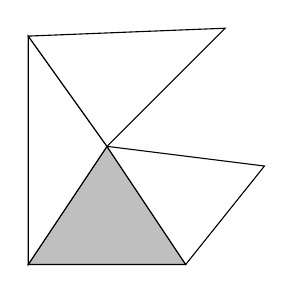
\begin{tikzpicture}
    \coordinate (A) at (0,0);   \coordinate (B) at (2,0); \coordinate (C) at (1,1.5);
    \coordinate (D) at (0,2.9); \coordinate (E) at (2.5,3); \coordinate (F) at (3,1.25); 
    \draw[fill=gray!50] (A) -- (B) -- (C) -- cycle; 
    \draw[fill=white  ] (A) -- (C) -- (D) -- cycle; 
    \draw[fill=white  ] (C) -- (D) -- (E) -- cycle; 
    \draw[fill=white  ] (B) -- (C) -- (F) -- cycle; 
\end{tikzpicture}
\quad
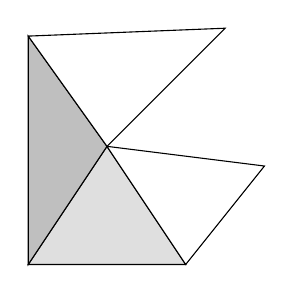
\begin{tikzpicture}
    \coordinate (A) at (0,0);   \coordinate (B) at (2,0); \coordinate (C) at (1,1.5);
    \coordinate (D) at (0,2.9); \coordinate (E) at (2.5,3); \coordinate (F) at (3,1.25); 
    \draw[fill=gray!25] (A) -- (B) -- (C) -- cycle; 
    \draw[fill=gray!50] (A) -- (C) -- (D) -- cycle; 
    \draw[fill=white  ] (C) -- (D) -- (E) -- cycle; 
    \draw[fill=white  ] (B) -- (C) -- (F) -- cycle; 
\end{tikzpicture}
\quad
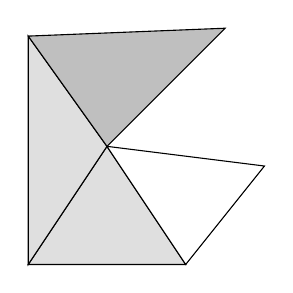
\begin{tikzpicture}
    \coordinate (A) at (0,0);   \coordinate (B) at (2,0); \coordinate (C) at (1,1.5);
    \coordinate (D) at (0,2.9); \coordinate (E) at (2.5,3); \coordinate (F) at (3,1.25); 
    \draw[fill=gray!25] (A) -- (B) -- (C) -- cycle; 
    \draw[fill=gray!25] (A) -- (C) -- (D) -- cycle; 
    \draw[fill=gray!50] (C) -- (D) -- (E) -- cycle; 
    \draw[fill=white  ] (B) -- (C) -- (F) -- cycle; 
\end{tikzpicture}
\quad
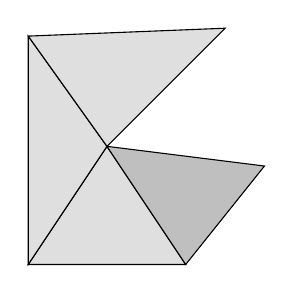
\begin{tikzpicture}
    \coordinate (A) at (0,0);   \coordinate (B) at (2,0); \coordinate (C) at (1,1.5);
    \coordinate (D) at (0,2.9); \coordinate (E) at (2.5,3); \coordinate (F) at (3,1.25); 
    \draw[fill=gray!25] (A) -- (B) -- (C) -- cycle; 
    \draw[fill=gray!25] (A) -- (C) -- (D) -- cycle; 
    \draw[fill=gray!25] (C) -- (D) -- (E) -- cycle; 
    \draw[fill=gray!50] (B) -- (C) -- (F) -- cycle; 
\end{tikzpicture}
\end{center}
\caption{Exhausting a domain step by step as in Theorem~\ref{theorem:poincarefriedrichsestimate:grad} and \ref{theorem:poincarefriedrichsestimate:gradzwei}.
The dark gray triangle is the one being currently added, and the light gray triangles constitute the subdomain assembled so far.}
\label{figure:exhausting}
\end{figure}

\begin{remark}
    Theorem~\ref{theorem:poincarefriedrichsestimate:grad} depends on only a few parameters of the triangulation:
    the length of any traversal from the root simplex, the ratios of the volumes of adjacent simplices,
    the Poincar\'e--Friedrichs constants on each face patch, and the Poincar\'e--Friedrichs constant of the initial simplex. 
    The aforementioned local Poincar\'e--Friedrichs constants can generally be estimated in terms of shape-parameters. 
    If the face patches of the triangulation are convex, then better estimates are possible. 
\end{remark}

We write $\Omega_{m} \subseteq \bbR^{n}$ for the domain with $\overline\Omega_m := \cup_{j=0}^{m} T_m$, 
    which is a triangulated $n$-dimensional submanifold with boundary.
    \cye{\sout{We finally write $\Omega_m := \cup_{j=0}^{m} T_m$, which is a triangulated $n$-dimensional submanifold with boundary.}}
    \todo[inline]{MV: False, $\Omega_m$ is not necessarily a triangulated $n$-dimensional submanifold with boundary, see the 7-triangles example standing for $\Omega_m$ (then the 8th one gives $\Omega_{m+1} = \Omega$). As discussed online, we fortunately do not need here a submanifold with boundary (but we will need it and have it for shellable triangulations.) Actually, here we do not need $\Omega_m$ at all.}

    \mwl{Where to place that construction?}
 We construct the potential recursively. 
 We have seen that $c_{0} = w_{0} - u_{|\Omega_{0}}$ is a constant. 
 Assume that $1 \leq m \leq M$ such that there exists $w_{\iota(m)} \in W^{1,p}(\Omega_{\iota(m)})$ 
 such that $c_{0} = w_{\iota(m)} - u_{|\Omega_{\iota(m)}}$ is the constant above. 
 % Note that this assumption is already satisfied when $m=1$.
 Hence $\nabla w_{\iota(m)} = \nabla u$ over $\Omega_{\iota(m)}$. 
 By assumption, $T_{m}$ shares the face $F_{m}$ with $T_{{\iota(m)}}$. 
 Since $$\nabla w_{F_{m}|T_{{\iota(m)}}} = \nabla w_{\iota(m)|T_{{\iota(m)}}},$$
 there exists a constant $$c_{m} := w_{\iota(m)|T_{{\iota(m)}}} - w_{F_{m}|T_{{\iota(m)}}}.$$
 We define $w'_{F_m} := w_{F_m} + c_{m} \in W^{1,p}(U_F)$.
 By construction, $$\nabla w'_{F_m} = \nabla w_{F_m} = \nabla u_{|U_{F_m}}$$ 
 and 
 $w'_{F_{m}|T_{{\iota(m)}}} = w_{\iota(m)|T_{{\iota(m)}}}$. 
 But that already implies $w'_{F_m} = w_{|F_m} - c_{0}$. 
 Defining $w_{m} \in W^{1,p}(\Omega_m)$ by extending $w_{\iota(m)}$ with $w'_{F_m|T_m}$,
 we have $c_{0} = w_{m} - u_{|\Omega_{m}}$. 

  
 
 \mwl{Closure}
 We obtain the desired estimate. 
 Repeating this argument produces $w \in L^{p}(\Omega)$ 
 such that for all $n$-simplices $T \in \calT$ we have the restriction $w_{|T} \in W^{1,p}(T)$ with $w_{|T} = u + c_{0}$.
 In particular, $w \in W^{1,p}(\Omega)$ with $\nabla w = \nabla u$.
 
 
 
 
 
 
 
 
 
\begin{figure}
    \centering
    \begin{tabular}{c}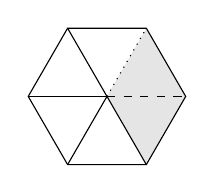
\begin{tikzpicture}
        \coordinate (O) at (0, 0);
        \coordinate (A) at ({cos(0)}, {sin(0)});
        \coordinate (B) at ({cos(60)}, {sin(60)});
        \coordinate (C) at ({cos(120)}, {sin(120)});
        \coordinate (D) at ({cos(180)}, {sin(180)});
        \coordinate (E) at ({cos(240)}, {sin(240)});
        \coordinate (F) at ({cos(300)}, {sin(300)});
        \fill[gray!20] (A) -- (B) -- (O) -- (F) -- cycle;
        \draw (A) -- (B) -- (C) -- (D) -- (E) -- (F) -- cycle;
        \draw[dashed] (O) -- (A); \draw[dotted] (O) -- (B); \draw (O) -- (C); \draw (O) -- (D); \draw (O) -- (E); \draw (O) -- (F);
    \end{tikzpicture}\\ (1) \end{tabular}
    \begin{tabular}{c}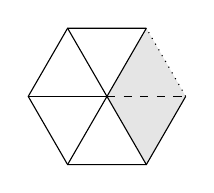
\begin{tikzpicture}
        \coordinate (O) at (0, 0);
        \coordinate (A) at ({cos(0)}, {sin(0)});
        \coordinate (B) at ({cos(60)}, {sin(60)});
        \coordinate (C) at ({cos(120)}, {sin(120)});
        \coordinate (D) at ({cos(180)}, {sin(180)});
        \coordinate (E) at ({cos(240)}, {sin(240)});
        \coordinate (F) at ({cos(300)}, {sin(300)});
        \fill[gray!20] (A) -- (B) -- (O) -- (F) -- cycle;
        \draw[dotted] (A) -- (B); \draw (B) -- (C) -- (D) -- (E) -- (F) -- (A);
        \draw[dashed] (O) -- (A); \draw (O) -- (B); \draw (O) -- (C); \draw (O) -- (D); \draw (O) -- (E); \draw (O) -- (F);
    \end{tikzpicture}\\ (2) \end{tabular}
    \begin{tabular}{c}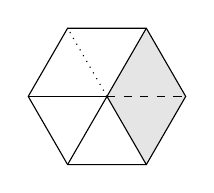
\begin{tikzpicture}
        \coordinate (O) at (0, 0);
        \coordinate (A) at ({cos(0)}, {sin(0)});
        \coordinate (B) at ({cos(60)}, {sin(60)});
        \coordinate (C) at ({cos(120)}, {sin(120)});
        \coordinate (D) at ({cos(180)}, {sin(180)});
        \coordinate (E) at ({cos(240)}, {sin(240)});
        \coordinate (F) at ({cos(300)}, {sin(300)});
        \fill[gray!20] (A) -- (B) -- (O) -- (F) -- cycle;
        \draw (A) -- (B) -- (C) -- (D) -- (E) -- (F) -- cycle;
        \draw[dashed] (O) -- (A); \draw (O) -- (B); \draw[dotted] (O) -- (C); \draw (O) -- (D); \draw (O) -- (E); \draw (O) -- (F);
    \end{tikzpicture}\\ (3) \end{tabular}
    \begin{tabular}{c}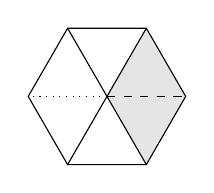
\begin{tikzpicture}
        \coordinate (O) at (0, 0);
        \coordinate (A) at ({cos(0)}, {sin(0)});
        \coordinate (B) at ({cos(60)}, {sin(60)});
        \coordinate (C) at ({cos(120)}, {sin(120)});
        \coordinate (D) at ({cos(180)}, {sin(180)});
        \coordinate (E) at ({cos(240)}, {sin(240)});
        \coordinate (F) at ({cos(300)}, {sin(300)});
        \fill[gray!20] (A) -- (B) -- (O) -- (F) -- cycle;
        \draw (A) -- (B) -- (C) -- (D) -- (E) -- (F) -- cycle;
        \draw[dashed] (O) -- (A); \draw (O) -- (B); \draw (O) -- (C); \draw[dotted] (O) -- (D); \draw (O) -- (E); \draw (O) -- (F);
    \end{tikzpicture}\\ (4) \end{tabular}
    \caption{Examples and counterexamples for building a manifold-like $1$-patching of a $2$-dimensional manifold-like triangulation. 
    (1) We have already added the edge patch along the dashed line and we add the edge patch along the dotted line.
    (2) The new edge patch may already be a subset of the subtriangulation
    (3) An inadmissible choice because the new edge patch has no overlap with current subtriangulation, though the next subtriangulation would be manifold-like
    (4) An inadmissible choice because the new edge patch has no overlap with current subtriangulation and the next subtriangulation would not be manifold-like.}\label{figure:illustrationpatching}
\end{figure}

% \begin{figure}
%     \centering
%     \begin{tabular}{c}\begin{tikzpicture}[scale=0.5]
%         \coordinate (O) at (0, 0);
%         \coordinate (A) at ({0.8*cos(  0)}, {0.8*sin(  0)});
%         \coordinate (B) at ({0.8*cos(120)}, {0.8*sin(120)});
%         \coordinate (C) at ({0.8*cos(240)}, {0.8*sin(240)});
%         \coordinate (X) at ({3.0*cos( 60)}, {3.0*sin( 60)});
%         \coordinate (Y) at ({3.0*cos(180)}, {3.0*sin(180)});
%         \coordinate (Z) at ({3.0*cos(300)}, {3.0*sin(300)});
%         \draw (A) -- (B) -- (C) -- cycle; \draw (X) -- (Y) -- (Z) -- cycle;
%         \draw[fill=gray!20] (X) -- (Y) -- (B) -- cycle;
%         \draw[fill=gray!20] (Y) -- (Z) -- (C) -- cycle;
%         \draw[fill=gray!20] (Z) -- (X) -- (A) -- cycle;
%         \draw[fill=gray!20] (A) -- (X) -- (B) -- cycle;
%         \draw[fill=gray!20] (B) -- (Y) -- (C) -- cycle;
%         \draw[fill=gray!20] (C) -- (Z) -- (A) -- cycle;
%     \end{tikzpicture}\\ (1) \end{tabular}
%     \begin{tabular}{c}\begin{tikzpicture}[scale=0.5]
%         \coordinate (O) at (0, 0);
%         \coordinate (A) at ({3.0*cos(  0)}, {3.0*sin(  0)});
%         \coordinate (B) at ({3.0*cos(120)}, {3.0*sin(120)});
%         \coordinate (C) at ({3.0*cos(240)}, {3.0*sin(240)});
%         \coordinate (X) at ({3.0*cos( 60)}, {3.0*sin( 60)});
%         \coordinate (Y) at ({3.0*cos(180)}, {3.0*sin(180)});
%         \coordinate (Z) at ({3.0*cos(300)}, {3.0*sin(300)});
%         \draw (O) -- (A);
%         \draw (O) -- (B);
%         \draw (O) -- (C);
%         \draw (O) -- (X);
%         \draw (O) -- (Y);
%         \draw (O) -- (Z);
%         %
%     \end{tikzpicture}\\ (2) \end{tabular}
%     \begin{tabular}{c}\begin{tikzpicture}[scale=0.5]
%         \tikzset{z={(90:1cm)}, y={(-30:1cm)}, x={(210:1cm)}}
%         % \tikzset{z={(90:1cm)}, y={(-10:1cm)}, x={(250:1cm)}}
% 
%         \coordinate (O) at (0, 0);
%         \coordinate (A) at ({3.0*cos(  0)}, {3.0*sin(  0)});
%         \coordinate (B) at ({3.0*cos(120)}, {3.0*sin(120)});
%         \coordinate (C) at ({3.0*cos(240)}, {3.0*sin(240)});
%         \coordinate (X) at ({3.0*cos( 60)}, {3.0*sin( 60)});
%         \coordinate (Y) at ({3.0*cos(180)}, {3.0*sin(180)});
%         \coordinate (Z) at ({3.0*cos(300)}, {3.0*sin(300)});
%         \coordinate (T) at ({0}, {0}, {3});
% 
%         \draw[thick, fill=gray!30] (O) -- (C) -- (T) -- cycle;
%         \draw[thick, fill=gray!30] (O) -- (Y) -- (T) -- cycle;
%         \draw[thick, fill=gray!30] (O) -- (Z) -- (T) -- cycle;
%         \draw[thick, fill=gray!30] (O) -- (A) -- (T) -- cycle;
%         \draw[thick, fill=gray!30] (O) -- (B) -- (T) -- cycle;
%         \draw[thick, fill=gray!30] (O) -- (X) -- (T) -- cycle;
% 
%     \end{tikzpicture}\\ (3) \end{tabular}
%     \caption{Example of a connected $2$-dimensional manifold triangulation, which triangulates an annulus, that does neither admit a manifold-like $0$-patching nor manifold-like $1$-patching.}\label{figure:annuluscounterexample}
% \end{figure}
 






        \color{blue}
        We study the singular values of the matrix 
        \begin{align*}
            \begin{pmatrix}
            -1                 & 0
            \\ 
            -2 \|b_z\|/\|h_z\| & 1
            \end{pmatrix}
            =
            \begin{pmatrix}
            -1             & 0
            \\ 
            -2 \tan(\beta) & 1
            \end{pmatrix}
            =
            \begin{pmatrix}
            0             & \tan(\beta)
             \\ 
            -\tan(\beta) & 0
            \end{pmatrix}
            +
            \begin{pmatrix}
            -1           & -\tan(\beta)
             \\ 
            \tan(\beta) & 1
            \end{pmatrix}
            .
        \end{align*}
        It follows that $\det(\Theta_{|K}) = 1$. 
        Its singular values satisfy 
        \begin{align*}
            ( \sigma_{\max} + \sigma_{\min} )/2
            =
            \tan(\beta)
            ,
            \qquad 
            ( \sigma_{\max} - \sigma_{\min} )/2
            =
            \sqrt{ 1 + \tan^{2}(\beta) }
            .
        \end{align*}
        We arrive at 
        \begin{align*}
            \sigma_{\max} = \sqrt{ 1 + \tan^{2}(\beta) } + \tan(\beta)
            ,
            \qquad 
            \sigma_{\min} = \sqrt{ 1 + \tan^{2}(\beta) } - \tan(\beta)
            .
        \end{align*}
\begin{align*}
    \lambda^2 = \frac{1}{2} \left( a + c \pm \sqrt{ a^2 - 2 a c + c^2 + 4b^2 } \right)
\end{align*}
\begin{align*}
    \lambda 
    &= 
    \frac{1}{\sqrt 2} \sqrt{ (1+t^2) + 1 \pm \sqrt{ (1+t^2)^2 - 2 (1+t^2)   +   1 + 4t^2 } } 
    \\
    &= 
    \frac{1}{\sqrt 2} \sqrt{ t^2 + 2 \pm \sqrt{ 1 + 2t^2 + t^4 - 2 - 2 t^2 + 1 + 4t^2 } } 
    \\
    &= 
    \frac{1}{\sqrt 2} \sqrt{ t^2 + 2 \pm \sqrt{          + t^4                 + 4t^2 } } 
    \\
    &= 
    \frac{1}{\sqrt 2} \sqrt{ t^2 + 2 \pm t \sqrt{ t^2 + 4 } } 
    .
\end{align*}
\begin{align*}
    \lambda = \frac{1}{\sqrt 2} \sqrt{ t^2 + 2 \pm t \sqrt{ t^2 + 4 } } 
\end{align*}
\begin{align*}
    \left( t^2 + 2 + t \sqrt{ t^2 + 4 } \right)
    \left( t^2 + 2 - t \sqrt{ t^2 + 4 } \right)
    =
    t^{4} + 4 t^{2} + 4
    -
    t^{2} ( t^{2} + 4 )
    =
    4
\end{align*}
\begin{align*}
    \frac{1}{\sqrt 2} \sqrt{ t^2 + 2 \pm t \sqrt{ t^2 + 4 } } 
    &=
    \sqrt{1+a^2/4} \pm a/2
    \\
    \frac 1 2 \left( t^2 + 2 \pm t \sqrt{ t^2 + 4 } \right)
    &=
    1+a^2/4
    \pm
    a \sqrt{1+a^2/4}
    + 
    a^2/4
    \\&=
    1
    +
    2a^2/4
    \pm
    a \sqrt{1+a^2/4}
    \\
    1 + \frac{t^2}{2} \pm t \sqrt{ \frac{t^2}{4} + 1 } 
    &=
    1
    +
    a^2/2
    \pm
    a \sqrt{1+a^2/4}
    .
\end{align*}
\color{black}



















\begin{itemize}
        \item 
        % \todo{Combine all this to get the final transformation.}
        The last simplicial complex that we introduce is called $\calK$,
        and it is the simplicial complex obtained from $\patch_{\calT}(S)$ via barycentric refinement of $S$. 
        
        We let $\calK$ the simplicial complex obtained from $\patch_{\calT}(S)$ via barycentric refinement of $S$. 
        Using our initial observations, we obtain homeomorphisms 
        \begin{align*}
            \Psi_{\calK } : |\calK| \rightarrow \calB,
            \qquad 
            \Psi_{\calR'} : |\calR'| \rightarrow \calB.
        \end{align*}
        Both $\Psi_{\calK}$ and $\Psi_{\calR'}$ map $T$ onto the same subset of the unit ball.
        Consequently, the image under $\Psi_{\calK}$ of $\overline{|\calK| \setminus T}$
        onto the image under $\Psi_{\calR'}$ of $|\calR^{c}|$.
        It follows that 
        \begin{align*}
            \Xi_{S} := \Psi_{\calK}^{-1} \Psi_{\calR'} \Theta
        \end{align*}
        is a mapping from $T$ onto $\overline{\patch_{\calT}(S) \setminus T}$.
        We estimate the Jacobians: 
        \begin{align*}
            \| \Jacobian \Xi_{S} \| 
            \leq 
            \sup_{ K \in \calK  }
            \left( 1 + n \kappa(A_{K})^{2} \right)^{\frac 1 2}
            \sigma_{\max}(A_{K}) 
            %
            \sup_{ K \in \calR' } 
            \sqrt{2n} 
            \sigma_{\max}(A_{K}^{-1}) 
            %
            \sup_{ K \in \calR  } \kappa(A_{K})
            \\
            \| \Jacobian \Xi_{S}^{-1} \| 
            \leq 
            \sup_{ K \in \calK  }
            \sqrt{2n} 
            \sigma_{\max}(A_{K}^{-1}) 
            %
            \sup_{ K \in \calR' } 
            \left( 1 + n \kappa(A_{K})^{2} \right)^{\frac 1 2}
            \sigma_{\max}(A_{K}) 
            %
            \sup_{ K \in \calR  } \kappa(A_{K})
            .
        \end{align*}
        \color{red}
        Each bisection step reduces the diameter by at most a factor of one half,
        and it reduces the volume always by a factor of one half. 
        Via the estimates in Lemma~\ref{lemma:affinetransform}, we thus find 
        \begin{align*}
            \| \Jacobian \Xi_{S} \| 
            &\leq 
            2 \left( \sqrt{n} + 1 \right) 
            \sup_{ K \in \calK  }
            \Ceins{n} \diam(K) 
            \sup_{ K \in \calR' } 
            \Czwei{n} \kappa(K) \diam(K)^{-1}
            \sup_{ K \in \calR  } \kappa(A_{K})
            \\&\leq 
            32 \left( \sqrt{n} + 1 \right) 
            \theta(\calT)
            \Ceins{n} 
            \Czwei{n} 
            \kappa(\calT) 
            \alpha(\calT)
            \\
            \| \Jacobian \Xi_{S}^{-1} \| 
            &\leq 
            2 \left( \sqrt{n} + 1 \right) 
            \sup_{ K \in \calK  }
            \Czwei{n} \kappa(K) \diam(K)^{-1}
            \sup_{ K \in \calR' } 
            \Ceins{n} \diam(K)
            \sup_{ K \in \calR  } \kappa(A_{K})
            \\
            &\leq 
            32 \left( \sqrt{n} + 1 \right) 
            \theta(\calT)
            \Ceins{n} 
            \Czwei{n} 
            \kappa(\calT) 
            \alpha(\calT)
            .
        \end{align*}
        Together with the definition of $\theta(\calT)$, the desired result follows. 
%         \color{red}
%         Each bisection halves the volume of the triangles. Thus,
%         \begin{align*}
%             \| \Jacobian \Xi_{S} \| 
%             &\leq 
%             2 
%             \sup_{ K \in \patch_{\calT}(S) }
%             2 \sigma_{\max}(A_{K}) 
%             4 
%             \left( \sqrt{n} + 1 \right) \sigma_{\max}(A_{T}^{-1}) 
%             4 
%             \kappa(A_{T})
%             \\&\leq 
%             64
%             \left( \sqrt{n} + 1 \right) 
%             \kappa(A_{T})
%             \sigma_{\max}(A_{T}^{-1}) 
%             \sup_{ K \in \patch_{\calT}(S) }
%             \sigma_{\max}(A_{K}     ) 
%             \\
%             \| \Jacobian \Xi_{S}^{-1} \| 
%             &\leq 
%             2 \left( \sqrt{n} + 1 \right) 
%             \sup_{ K \in \patch_{\calT}(S) }
%             \sigma_{\max}(A_{K}) 
%             \sigma_{\max}(A_{T}^{-1}) 
%             4 \kappa(A_{T})
%             \\&\leq 
%             64
%             \left( \sqrt{n} + 1 \right) 
%             \kappa(A_{T})
%             \sigma_{\max}(A_{T}^{-1}) 
%             \sup_{ K \in \patch_{\calT}(S) }
%             \sigma_{\max}(A_{K}     ) 
%             .
%         \end{align*}
%         We use 
%         \begin{gather*}
%             \sup_{ K \in \patch_{\calT}(S) }
%             \sigma_{\max}(A_{K}) 
%             \leq 
%             \Ceins{n} 
%             \sup_{ K \in \patch_{\calT}(S) }
%             \diam(K)
%             \leq 
%             \Ceins{n} 
%             \theta(\calT)
%             \sigma_{\max}(A_{T}) 
%             .
%         \end{gather*}
%         \color{black}
        % That establishes the final estimate. 
%         \item 
%         Suppose that $S = \{v_0\}$ is a single vertex. 
%         We construct a transformation from the vertex star around $S$ onto the Euclidean unit ball. 
%         Without loss of generality, $S$ is at the origin. 
%         For any $T \in \patch_{\calT}(S)$, we let $F_T$ be the transformation. 
%         We define $F$ over $|\patch_{\calT}(S)|$ piecewise. 
%         \todo{Complete}
%         
        
%         \item 
%         Let $\calU$ be the simplicial complex of dimension $n-1$ that contains precisely those facets of $T$ that do not contain $S$.
%         We write $Y := F( |\calU| )$. 
%         \todo{Shape of the outer patch $Y$, star-shaped geometry}
%         
%         \item 
%         We let $\sphere{n}_{\star} := \sphere{n} \setminus \{e_{n+1}\} \subseteq \bbR^{n+1}$ be the unit sphere without the North pole. 
%         Suppose that $\bar x \in \sphere{n}$ is a point on the unit sphere and $\bar x \neq e_{n+1}$. 
%         We define its stereographic projection as 
%         \begin{align*}
%             \pi( \bar x ) 
%             = 
%             \sum_{i=1}^{n} \frac{x_i}{1 - x_{n+1}} e_{i}
%             .
%         \end{align*}
%         This is a mapping $\pi : \sphere{n}_{\star} \rightarrow \bbR^{n}$. 
%         Its inverse is defined as follows: given $y \in \bbR^{n}$, we have 
%         \begin{align*}
%             \pi^{-1}( y )
%             = 
%             \sum_{i=1}^{n} \frac{2 y_i}{1 + \| y \|^2} e_{i}
%             +
%             \frac{1 - \| y \|^2}{1 + \| y \|^2} e_{n+1}
%             .
%         \end{align*}
%         \item 
%         Mirroring the unit sphere along the equator is expressed in stereographic coordinates by the involution 
%         \begin{align*}
%             \mu : \bbR^{n} \rightarrow \bbR^{n},
%             \qquad 
%             y \mapsto \frac{y}{\| y \|}.
%         \end{align*}
%         \item 
%         \begin{align*}
%             G(y) := \| y \| \cdot \phi\left( \frac{y}{\|y\|} \right)^{-1} \frac{y}{\|y\|}
%         \end{align*}
%         \item 
%         We combine these mappings:
%         \begin{align*}
%             Q : \sphere{n} \rightarrow \sphere{n}, \qquad x \mapsto \pi^{-1} G^{-1} \mu G \pi(x)
%         \end{align*}
%         We want to analyze its Lipschitz properties. \todo{Stuff}
%         \item
%         We have constructed a bi-Lipschitz mapping from the Euclidean unit sphere into itself.
%         We use the following result~\cite[Theorem~3]{alestalo2018radial}:
%         if $f : \sphere{n} \rightarrow \sphere{n}$ is any $L$-Lipschitz mapping from the Euclidean unit sphere into itself, 
%         then the radial extension $f : \ball{n} \rightarrow \ball{n}$ is an $L$-Lipschitz mapping from the Euclidean unit ball into itself.
%         Consequently, \todo{write out}
%         \item 
%         In total, we thus have 
%         \begin{align*}
%             Q' := F^{-1} \pi^{-1} G^{-1} \mu G \pi F
%             .
%         \end{align*}




        \item 
        We begin with the following preparatory observations. 
        Consider any $n$-simplex $T$ with vertices $v_0, v_1, \dots, v_n$, where $v_0$ is the origin. 
        We let $A_{T} \in \bbR^{n \times n}$ be the matrix that maps the $i$-th unit vector to $v_i$.
        That matrix maps the reference simplex $\Delta^{n}$ onto $T$. 
        Then the mapping 
        \begin{align}
            F_T(x) 
            = 
            \frac{ \| A_{T}^{-1} x \|_{1} }{ \|x\|_2 } x
        \end{align}
        maps $T$ onto a ``simplex with a curved face'' inside the Euclidean unit ball. Its inverse is
        \begin{align}
            F_T^{-1}(x) 
            = 
            \frac{ \|x\|_2 }{ \| A_{T}^{-1} x \|_{1} } x
            .
        \end{align}
        We analyze its Lipschitz properties.
        % 
        In what follows, $y \in \bbR^{n}$. 
        On the one hand, 
        we compute the Jacobian at any $x \in \mathring T$:
        \begin{align*}
            \Jacobian F_T(x) \cdot y
            &= 
            \frac{ \|x\| y - x \|x\|^{-1} x^t y }{\|x\|^2} 
            \left( \vecone \cdot A_{T}^{-1} x \right)
            + 
            \frac{x}{\|x\|} \left( \vecone \cdot A_{T}^{-1} y \right)
            \\&= 
            \left( \Id - \|x\|^{-2} x \otimes x^t \right)
            \frac{ 1 }{ \|x\| } 
            \left( \vecone \cdot A_{T}^{-1} x \right)
            + 
            \frac{x}{\|x\|} \left( \vecone \cdot A_{T}^{-1} x \right)
            \\&= 
            \left( A_{T}^{-t} \vecone \cdot \hat x \right)
            \left( \Id - \hat x \otimes \hat x^t \right) y
            + 
            \left( A_{T}^{-t} \vecone \cdot y \right) \hat x 
            .
        \end{align*}
        This is an orthogonal sum of two vectors. Its norm satisfies:
        \begin{align*}
            \| \Jacobian F_T(x) \cdot y \|^{2}
            &= 
            \left| A_{T}^{-t} \vecone \cdot \hat x \right|^{2}
            \| \left( \Id - \hat x \otimes \hat x^t \right) y \|^{2}
            + 
            \left| A_{T}^{-t} \vecone \cdot y \right|^{2} \| \hat x \|^{2}
            .
        \end{align*}
        The Euclidean operator norm satisfies 
        \begin{align*}
            \| \Jacobian F_T(x) \| 
            \leq 
            \sqrt 2 \left\| A_{T}^{-t} \vecone \right\|_{2}
            \leq 
            \sqrt{2n} \cdot \sigma_{\max}(A_{T}^{-1}) 
            .
        \end{align*}
        On the other hand, we can rewrite the Jacobian as:
        \begin{align*}
            \Jacobian F_T(x) \cdot y
            &= 
            \left( A_{T}^{-t} \vecone \cdot \hat x \right)
            y
            - 
            \left( A_{T}^{-t} \vecone \cdot \hat x \right)
            \left( \hat x \otimes \hat x^t \right) y
            + 
            \left( A_{T}^{-t} \vecone \cdot y \right) \hat x 
            \\&= 
            \left( A_{T}^{-t} \vecone \cdot \hat x \right)
            y
            - 
            \hat x 
            \left( 
                \left( A_{T}^{-t} \vecone \cdot \hat x \right) \hat x^{t}
                -
                \vecone^{t} A_{T}^{-1} 
            \right) y
            \\&= 
            \left( A_{T}^{-t} \vecone \cdot \hat x \right)
            y
            - 
            \hat x 
            \left( 
                \left( A_{T}^{-t} \vecone \cdot \hat x \right) \hat x
                -
                A_{T}^{-t} \vecone
            \right)^{t} y
            .
        \end{align*}
        Its inverse is found via the Woodbury formula: 
        % Its inverse is easily verified to be:
        \begin{align*}
            \Jacobian F_T(x)^{-1}
            &= 
            \left( A_{T}^{-t} \vecone \cdot \hat x \right)^{-1}
            \Id
            - 
            \left( A_{T}^{-t} \vecone \cdot \hat x \right)^{-2}
            \hat x 
            \left( 
                \left( A_{T}^{-t} \vecone \cdot \hat x \right) \hat x
                -
                A_{T}^{-t} \vecone
            \right)^{t} 
            \\&= 
            \left( A_{T}^{-t} \vecone \cdot \hat x \right)^{-1}
            \left( 
                \Id
                - 
                \hat x 
                \left( 
                    % \left( A_{T}^{-t} \vecone \cdot \hat x \right)^{-1}
                    % \left( A_{T}^{-t} \vecone \cdot \hat x \right) 
                    \hat x
                    -
                    \left( A_{T}^{-t} \vecone \cdot \hat x \right)^{-1}
                    A_{T}^{-t} \vecone
                \right)^{t}
            \right)
            \\&= 
            \left( \vecone \cdot A_{T}^{-1} \hat x \right)^{-1}
            \left( 
                \Id
                - 
                \hat x 
                \left( 
                    % \left( A_{T}^{-t} \vecone \cdot \hat x \right)^{-1}
                    % \left( A_{T}^{-t} \vecone \cdot \hat x \right) 
                    \hat x
                    -
                    \left( \vecone \cdot A_{T}^{-1} \hat x \right)^{-1}
                    A_{T}^{-t} \vecone
                \right)^{t}
            \right)
            \\&= 
            \left( \vecone \cdot A_{T}^{-1} \hat x \right)^{-1}
            \left( 
                \Id - \hat x \otimes \hat x^{t}
                + 
                \left( \vecone \cdot A_{T}^{-1} \hat x \right)^{-1}
                \hat x \otimes \vecone^{t} A_{T}^{-1}
            \right)
            .
        \end{align*}
        The inverse acts via multiplication with $\left( \vecone \cdot A_{T}^{-1} \hat x \right)^{-1}$ on the span of $\hat x$.
        We notice the upper bound 
        \begin{align*}
            \left( \vecone \cdot A_{T}^{-1} \hat x \right)^{-1}
            &= 
            \| A_{T}^{-1} \hat x \|^{-1}_{1}
            \\&\leq  
            \| A_{T}^{-1} \hat x \|^{-1}_{2}
            \leq 
            \sigma_{\min}( A_{T}^{-1} )^{-1}
            = 
            \sigma_{\max}( A_{T} )
            .
        \end{align*}
        This holds because $A_{T}^{-1} \hat x$ is in the positive quadrant.
        %, and its scalar product with $\vecone$ is minimized when it is colinear with a coordinate axis.
        If $y \in \bbR^{n}$ is orthogonal to $\hat x$, then 
        \begin{align*}
            \| \Jacobian F_T(x)^{-1} \cdot y \|^{2}
            &\leq 
%             \left( \vecone \cdot A_{T}^{-1} \hat x \right)^{-2}
%             \left\| 
%                 y
%             \right\|^{2}
%             +
%             \left( \vecone \cdot A_{T}^{-1} \hat x \right)^{-2}
%             \left| 
%                 \left( \vecone \cdot A_{T}^{-1} \hat x \right)^{-1}
%                 \vecone^{t} A_{T}^{-1} y 
%             \right|^{2}
%             \\&\leq 
            \left( \vecone \cdot A_{T}^{-1} \hat x \right)^{-2}
            \left\| 
                y
            \right\|^{2}
            +
            \frac{ 
            \left| 
                \left( \vecone \cdot A_{T}^{-1} \hat x \right)^{-1}
                \vecone^{t} A_{T}^{-1} y 
            \right|^{2}
            }{
            \left( \vecone \cdot A_{T}^{-1} \hat x \right)^{2}
            }
            .
        \end{align*}
        The operator norm of that inverse is:
        \begin{align*}
            \| \Jacobian F_T(x)^{-1} \|
            \leq 
            \sigma_{\max}( A_{T} )
            \left( 1 + n \frac{ \sigma_{\max}(A_{T})^{2} }{ \sigma_{\min}(A_{T})^{2} } \right)^{\frac 1 2}
            .
        \end{align*}
        Since the domain and codomain of $F_{T}$ are convex, 
        this also implies bounds on the Lipschitz constants of $F_{T}$ and its inverse. 











\color{red}
        On the one hand, given $x, y \in T$, 
        where $\| y \|_{1} \leq \| x \|_{1}$ without loss of generality, we find 
        \begin{align*}
            &
            \left\| F_T(x) - F_T(y) \right\|_{2}
            \\&\qquad 
            \leq 
            \left\| 
                \frac{ \| A_{T}^{-1} x \|_{1} }{ \|x\|_2 } x - \frac{ \| A_{T}^{-1} y \|_{1} }{ \|y\|_2 } y
            \right\|_{2}
            \\&\qquad 
            \leq 
            \left\| 
                \frac{ \| A_{T}^{-1} x \|_{1} }{ \|x\|_2 } x - \frac{ \| A_{T}^{-1} x \|_{1} }{ \|x\|_2 } y
            \right\|_{2}
            +
            \left\| 
                \frac{ \| A_{T}^{-1} x \|_{1} }{ \|x\|_2 } y - \frac{ \| A_{T}^{-1} y \|_{1} }{ \|y\|_2 } y
            \right\|_{2}
            \\&\qquad 
            \leq 
            \frac{ \| A_{T}^{-1} x \|_{1} }{ \|x\|_2 } 
            \left\| 
                x - y
            \right\|_{2}
            +
            \left| \|A_{T}^{-1} x\|_1 - \|A_{T}^{-1} y\|_1 \right|
            \\&\qquad 
            \leq 
            2\sqrt{n} \sigma_{\max}(A_{T}^{-1}) 
            \left\| x - y \right\|_{2}
            .
        \end{align*}
        On the one hand, given $x, y \in T$, 
        where $\| x \|_{2} \leq \| y \|_{2}$ without loss of generality, we find 
        \begin{align*}
            &
            \left\| F_T(x) - F_T(y) \right\|_{2}
            \\&\qquad 
            \leq 
            \left\| 
                \frac{ \| A_{T}^{-1} x \|_{1} }{ \|x\|_2 } x - \frac{ \| A_{T}^{-1} y \|_{1} }{ \|y\|_2 } y
            \right\|_{2}
            \\&\qquad 
            \leq 
            \left\| 
                \frac{ \| A_{T}^{-1} x \|_{1} }{ \|x\|_2 } x - \frac{ \| A_{T}^{-1} x \|_{1} }{ \|x\|_2 } y
            \right\|_{2}
            +
            \left\| 
                \frac{ \| A_{T}^{-1} x \|_{1} }{ \|x\|_2 } y - \frac{ \| A_{T}^{-1} y \|_{1} }{ \|x\|_2 } y
            \right\|_{2}
            +
            \left\| 
                \frac{ \| A_{T}^{-1} y \|_{1} }{ \|x\|_2 } y - \frac{ \| A_{T}^{-1} y \|_{1} }{ \|y\|_2 } y
            \right\|_{2}
            \\&\qquad 
            \leq 
            \frac{ \| A_{T}^{-1} x \|_{1} }{ \|x\|_2 } 
            \left\| 
                x - y
            \right\|_{2}
            +
            \left| \|A_{T}^{-1} x\|_1 - \|A_{T}^{-1} y\|_1 \right|
            \frac{\|y\|}{\|x\|}
            +
            \|A_{T}^{-1} y\|_1 \|y\|_{2}
            \left| \frac{1}{\|x\|} - \frac{1}{\|y\|} \right|
            \\&\qquad 
            \leq 
            \frac{ \| A_{T}^{-1} x \|_{1} }{ \|x\|_2 } 
            \left\| 
                x - y
            \right\|_{2}
            +
            \left| \|A_{T}^{-1} x\|_1 - \|A_{T}^{-1} y\|_1 \right|
            \frac{\|y\|}{\|x\|}
            +
            \|A_{T}^{-1} y\|_1 \|y\|_{2}
            \left| \frac{ \|y\|_{2} - \|x\|_{2} }{\|x\|_{2} \|y\|_{2}} \right|
            \\&\qquad 
            \leq 
            3 \sqrt{n} \sigma_{\max}(A_{T}^{-1}) 
            \left\| x - y \right\|_{2}
            .
        \end{align*}
        On the other hand, given $x, y \in F_T(T)$, 
        where $\| A_{T}^{-1} y \|_{1} \leq \| A_{T}^{-1} x \|_{1}$ without loss of generality, we find 
        \begin{align*}
            &
            \left\| F_T^{-1}(x) - F_T^{-1}(y) \right\|_{2}
            \\&\qquad 
            \leq 
            \left\| 
                \frac{ \|x\|_2 }{ \| A_{T}^{-1} x \|_{1} } x - \frac{ \|y\|_2 }{ \| A_{T}^{-1} y \|_{1} } y
            \right\|_{2}
            \\&\qquad 
            \leq 
            \left\| 
                \frac{ \|x\|_2 }{ \| A_{T}^{-1} x \|_{1} } x - \frac{ \|x\|_2 }{ \| A_{T}^{-1} x \|_{1} } y
            \right\|_{2}
            +
            \left\| 
                \frac{ \|x\|_2 }{ \| A_{T}^{-1} x \|_{1} } y - \frac{ \|y\|_2 }{ \| A_{T}^{-1} x \|_{1} } y
            \right\|_{2}
            +
            \left\| 
                \frac{ \|y\|_2 }{ \| A_{T}^{-1} x \|_{1} } y - \frac{ \|y\|_2 }{ \| A_{T}^{-1} y \|_{1} } y
            \right\|_{2}
            \\&\qquad 
            \leq 
            \frac{ \|x\|_2 }{ \| A_{T}^{-1} x \|_{1} } 
            \left\| 
                x - y
            \right\|_{2}
            +
            \left| \|x\|_2 - \|y\|_2 \right|
            \frac{ \|y\|_2 }{ \| A_{T}^{-1} x \|_{1} }
            +
            \|y\|_2^{2}
            \left| 
            \frac{ \| A_{T}^{-1} y \|_{1} - \| A_{T}^{-1} x \|_{1} }{ \| A_{T}^{-1} x \|_{1} \| A_{T}^{-1} y \|_{1} }
            \right|
            \\&\qquad 
            \leq 
            \frac{ \|x\|_2 }{ \| A_{T}^{-1} x \|_{2} } 
            \left\| 
                x - y
            \right\|_{2}
            +
            \left| \|x\|_2 - \|y\|_2 \right|
            \frac{ \|y\|_2 }{ \| A_{T}^{-1} x \|_{2} }
            +
            \|y\|_2^{2}
            \left| 
            \frac{ \| A_{T}^{-1} y \|_{1} - \| A_{T}^{-1} x \|_{1} }{ \| A_{T}^{-1} x \|_{2} \| A_{T}^{-1} y \|_{2} }
            \right|
            \\&\qquad 
            \leq 
            \left( 2 + \sqrt{n} \frac{\sigma_{\max}(A_{T}^{-1}) }{ \sigma_{\min}(A_{T}^{-1}) } \right) \sigma_{\min}(A_{T}^{-1})^{-1} 
            \left\| x - y \right\|_{2}
            \\&\qquad 
            \leq 
            \left( 2 + \sqrt{n} \kappa(A_{T}) \right) \sigma_{\max}(A_{T})
            \left\| x - y \right\|_{2}
            .
        \end{align*}
        By convexity of the range of $F_T(T)$, 
        we obtain a bound on the operator norm of the Jacobian of $F_{T}^{-1}$. 
        We recall that $\sigma_{\max}(A_{T}^{-1}) = \sigma_{\min}(A_{T})^{-1}$ and $\sigma_{\min}(A_{T}^{-1})^{-1} = \sigma_{\max}(A_{T})$.
        \color{black}
\item 
\end{itemize}











\begin{proof}
    We let $\hat F_0$ be the convex closure of the first $n$ unit vectors. 
    We let $\hat F_1, \dots, \hat F_n$ be the remaining faces of the reference simplex 
    such that the $i$-th coordinate equals zero along $\hat F_i$.

    Let $\varphi : \Delta^{n} \rightarrow T$ be an affine diffeomorphism 
    that maps the faces $\hat F_{0}, \hat F_{1}, \dots, \hat F_{l}$ onto the boundary patch $\Gamma$. 
    We let $\Upsilon^{n}$ be constructed by reflecting $\Delta^{n}$ across the coordinate axes $l+1$ through $n$.
    The boundary $\partial\Upsilon^{n}$ is the reflection of the faces $\hat F_{0}, \hat F_{1}, \dots, \hat F_{l}$ under that process. 
    Obviously, $\Upsilon^{n}$ is convex with diameter $2$. 


    Let $f = \cartan u$ with $u \in \bfW^{p}\Lambda^{k}(T)$.
    We set $\hat f := \varphi^{\ast} f$ and $\hat u = \varphi^{\ast} u$, 
    so that $\hat u \in \cartan \bfW^{p}\Lambda^{k}(\Delta^{n})$ and $\cartan \hat u = \hat f$.

    We construct $\tilde u \in L^{p}(\Upsilon^{n})$ as the reflection $\hat u$ across the coordinate axes $l+1$ through $n$, and we build $\tilde f \in L^{p}(\Upsilon^{n})$ analogously.
    Then $\tilde u \in \bfW^{p}(\Upsilon^{n})$ with $\cartan \tilde u = \tilde f$. 

    The operator norm bound of the potential operator shows 
    \begin{align*}
        \| \tilde u \|_{L^{p}(\Upsilon^{n})} 
        &\leq 
        n A(n,\ell) \frac{ \vol_{n}(B_2(0)) }{|\Upsilon^{n}|} 2 
        \| \tilde f \|_{L^{p}(\Upsilon^{n})}
        \\&
        \leq 
        2 n A(n,\ell) \vol_{n}(B_1(0)) \frac{ n! \cdot 2^{n} }{2^{n-l}} 
        \| \tilde f \|_{L^{p}(\Upsilon^{n})}
        .
    \end{align*}
    We use the pullback estimates 
    \begin{gather*}
        \| \tilde u \|_{L^{p}(\Upsilon^{n})} 
        \leq 
        \| \Jacobian\varphi \|_{\infty}^{k}
        |\det\varphi^{-\frac{1}{p}}|
        \cdot 
        \| \tilde u \|_{L^{p}(\Upsilon^{n})} 
        ,
        \\
        \| \tilde f \|_{L^{p}(\Upsilon^{n})} 
        \leq 
        2^{n-l}
        \| \hat f \|_{L^{p}(\hat T)} 
        \leq 
        2^{n-l}
        \| \Jacobian\varphi^{-1} \|_{\infty}^{k+1}
        |\det\varphi^{\frac{1}{p}}|
        \cdot 
        \| f \|_{L^{p}(T)} 
        .
    \end{gather*}
\end{proof}





\begin{remark}
    For reference, how the extension should work:
    suppose that $u \in H(\Omega)$ and let $f = du$.
    Suppose we have $u_1 \in H(T_1)$ with $du_1 = du$ over $T_1$. 
    We built $u'_2 \in H(T_2)$ such that 
    \begin{align*}
        \trace_F u_1 = \trace_F u'_2
    \end{align*}
    We let $u''_2 \in H(T_2)$ such that 
    \begin{align*}
        d u''_2 = f - d u'_2, \quad \trace_F u''_2 = 0
    \end{align*}
    Such $u''_2$ exists because 
    \begin{align*}
        \trace_F( f_2 - d u'_2 ) 
        &= 
        \trace_F f_1 - \trace_F d u'_2
        \\&= 
        \trace_F f_1 - \trace_F d u'_2
        \\&= 
        \trace_F d u_1 - \trace_F d u'_2
        \\&= 
        d \trace_F u_1 - d \trace_F u'_2
        \\&= 
        d \trace_F u_1 - d \trace_F u_1
        = 0
        .
    \end{align*}
    Setting $u_2 = u'_2 + u''_2$, we find 
    \begin{align*}
        d u_2 = d u'_2 + d u''_2 = d u'_2 + f - d u'_2 = f,
        \\
        \trace_F u_2 = \trace_F u'_2 = \trace_F u_1.
    \end{align*}
    That requires an extension from given partial boundary data. 
    Possible approaches:
    \begin{itemize}
        \item Reflect a neighborhood and multiply with cut-off function.
        \item Take traces from patch and extend onto new simplex. 
    \end{itemize}
\end{remark}








\begin{lemma}\label{lemma:mixedbconsimplex}
    Let $T$ be an $n$-simplex and with a face $F$. 
    If $u \in W^{1,p}(T)$ such that $\trace_{F} u = 0$, then 
    \begin{align*}
        \| u \|_{L^{p}(T)}
        &
        \leq 
        C_{{\rm PF},T,F,p} \| \nabla u \|_{L^{p}(T)}
    \end{align*}
    where $C_{{\rm PF},T,F,p} > 0$ is a constant such that 
    \begin{align*}
        C_{{\rm PF},T,F,p}
        \leq 
        \left( C_{{\rm PF},T,p} + \left( C_{{\rm PF},T,p}^{p} + p \cdot \diam(T) C_{{\rm PF},T,p}^{p-1} \right)^{\frac 1 p} \right),  
        \quad 
        C_{{\rm PF},T,F,p}
        \leq 
        \diam(T)
        .
    \end{align*}
\end{lemma}
\begin{proof}
    There exists $w \in W^{1,p}(T)$ with $\nabla w = \nabla u$ and 
    \[
        \| w \|_{L^{p}(T)}
        \leq 
        C_{{\rm PF},T,p} 
        \| \nabla w \|_{\bfL^{p}(T)}
        .
    \]
    Then $w-u$ is constant, and thus $\gamma := \trace_{F} (w-u) = \trace_{F} w$. 
    We use that 
    \[
        \| \gamma \|_{L^{p}(T)}
        =
        \gamma \vol(T)^\frac{1}{p}
        =
        \left( \frac{ \vol(T) }{ \vol(F) } \right)^\frac{1}{p}
        \cdot 
        \gamma 
        \vol(F)^\frac{1}{p}
        \leq 
        \left( \frac{ \vol(T) }{ \vol(F) } \right)^\frac{1}{p}
        \| \gamma \|_{L^{p}(F)}
        .
    \]
    Using a trace inequality~\cite[Lemma~2.8]{veeser2012poincare} when $1 \leq p < \infty$, we find 
    \begin{align*}
        \| \gamma \|_{L^{p}(F)}^{p}
        &
        \leq 
        \frac{ \vol(F) }{ \vol(T) }
        \| w \|_{L^{p}(T)}^{p}
        +
        p
        \cdot 
        \diam(T)
        \frac{ \vol(F) }{ \vol(T) }
        \| w \|_{L^{p}(T)}^{p-1}
        \| \nabla w \|_{L^{p}(T)}
        \\&
        \leq 
        \left( \frac{ \vol(F) }{ \vol(T) } \right)
        \left( C_{{\rm PF},T,p}^{p} + p \cdot C_{{\rm PF},T,p}^{p-1} \right) 
        \diam(T)^{p}
        \| \nabla w \|_{L^{p}(T)}^{p}
        \\&
        \leq 
        \left( \frac{ \vol(F) }{ \vol(T) } \right)
        \left( C_{{\rm PF},T,p}^{p} + p \cdot \diam(T) C_{{\rm PF},T,p}^{p-1} \right) 
        %\diam(T)^{p}
        \| \nabla w \|_{L^{p}(T)}^{p}
        .
    \end{align*}
    Recall that $u = w - \gamma$. The first inequality follows. 
    
    The second inequality follows from Rademachers theorem when $p = \infty$.
    Let assume that $1 \leq p < \infty$. 
    Suppose that $u \in C^{\infty}(T)$ with support disjoint from $F$.
    Without loss of generality, $F$ lies in the span of the first $n-1$ coordinates and the $n$-th coordinate is non-negative over $T$. 
    We write $\bfg \in \bfL^{\infty}(T)$ be the trivial extension of $u$ outside of $T$.
    With the fundamental theorem of calculus and H\"olders inequality: 
    \begin{align*}
        &
        \int_{\Omega} |u(x_{1},\dots,x_{n-1},x_{n})|^{p} dx_1 \dots dx_{n-1} dx_{n}
        \\&
        \leq
        \int_{\Omega} \left| \int_{0}^{x_n} \partial_{n} u(x_{1},\dots,x_{n-1},y) dy \right|^{p} dx_1 \dots dx_{n-1} dx_{n}
        \\&
        \leq
        \int_{\Omega} \int_{0}^{x_n} x_{n}^{p-1} \left| \partial_{n} u(x_{1},\dots,x_{n-1},y) \right|^{p} dy dx_1 \dots dx_{n-1} dx_{n}
        \\&
        \leq
        \int_{\Omega} \int_{0}^{D} D^{p-1} \left| \bfg(x_{1},\dots,x_{n-1},y) \right|^{p} dy dx_1 \dots dx_{n-1} dx_{n}
        \leq 
        D^{p} 
        \int_{\Omega} |\nabla u|^{p} dx
        .
    \end{align*}
    That $\|u\|_{L^{p}(\Omega)} \leq \diam(T) \|\nabla u\|_{L^{p}(\Omega)}$ for all $W^{1,p}(T)$ whose members have vanishing trace along $F$ follows from approximation via members of $u \in C^{\infty}(T)$ whose support is disjoint from $F$. 
    
    Very briefly verify that density argument: 
    There exists $\varphi : \hat T \rightarrow T_{m+1}$ mapping the convex closure of the $n$ unit vectors onto the face $F$.
    We let $\hat u := u \circ \varphi$ and define $\hat g \in \bfL^p(\hat T)$ via $\hat g := \nabla ( u \circ \varphi )$. 
    Then $\nabla \hat u = \hat g$. 
    % 
    Let $\hat U$ be the unit ball of the $\ell^1$ metric, which contains $\hat T$.
    We let $\tilde u$ be the extension of $\hat u$ onto $\hat U$ by reflection across the coordinate axes.
    We define $\tilde g = \nabla \tilde u$
    and see that $\tilde g$ is the extension of $\hat g$ onto $\hat U$ by reflection across the coordinate axes. 
    By construction $\tilde u$ vanishes at the boundary of $\hat U$,
    and we approximate $\tilde u$ in $W^{1,p}(\hat U)$ via a sequence in $C^{\infty}_{c}(\hat U)$. 
    
    
    There exists $\varphi : \hat T \rightarrow T_{m+1}$ mapping the convex closure of the $n$ unit vectors onto the face $F$.
    We let $\hat u := u \circ \varphi$ and define $\hat g \in \bfL^p(\hat T)$ via $\hat g := \nabla ( u \circ \varphi )$. 
    Then $\nabla \hat u = \hat g$. 
    % 
    Let $\hat U$ be the unit ball of the $\ell^1$ metric, which contains $\hat T$.
    We let $\tilde u$ be the extension of $\hat u$ onto $\hat U$ by reflection across the coordinate axes.
    We define $\tilde g = \nabla \tilde u$
    and see that $\tilde g$ is the extension of $\hat g$ onto $\hat U$ by reflection across the coordinate axes. 
    By construction $\tilde u$ vanishes at the boundary of $\hat U$, and thus Friedrichs inequality satisfies 
    \begin{gather*}
        \| \tilde u \|_{L^{p}(\hat U)} 
        \leq 
        2 
        \| \tilde g \|_{\bfL^{p}(\hat U)}
        .
    \end{gather*}
    In addition to that, 
    \begin{gather*}
        \| u \|_{L^{p}(T_{m+1})}
        \leq 
        |\det(\Dif \varphi)|^{\frac 1 p} 
        \| \hat u \|_{L^{p}(\hat T)}
        \leq 
        |\det(\Dif \varphi)|^{\frac 1 p} 
        \| \tilde u \|_{L^{p}(\hat U)}
        ,
        \\
        \| \tilde g \|_{\bfL^{p}(\hat U)}
        \leq 
        2^{\frac n p}
        \| \hat g \|_{\bfL^{p}(\hat T)}
        \leq 
        2^{\frac n p}
        |\det(\Dif \varphi_1)|^{-\frac 1 p} \| \Dif \varphi \| \cdot 
        \| \nabla u \|_{\bfL^{p}(T)}
        .
    \end{gather*}
    The second inequality follows.
\end{proof}







Given $a \in \Omega$, we introduce the potential operator 
\begin{align*}
    \Poinc_{\ell,a} u(x) 
    &:= 
    (x-a)\lrcorner \int_{0}^{1} t^{\ell-1} u\left(a+t(x-a)\right)\,dt\;
    .
\end{align*}
By definition,
\begin{align*}
    \Poinc_{\ell} u(x) 
    =
    \int_{\Omega} \Poinc_{\ell,a} u(x) \,da\;
    .
\end{align*}
We study the interaction of the potential operator with the exterior derivative in more detail.
Suppose that $u \in C^{\infty}(\bbR^n,\Alt^{\ell})$ with $\supp u \subseteq \overline\Omega$.
We rewrite the potential,
\begin{align*}
    \Poinc_{\ell,a} u(x) 
    &= 
    (x-a)\lrcorner \int_{0}^{1} t^{\ell-1} u\left(a+t(x-a)\right)\,dt\,da\;
    \\&
    = 
    (x-a)\lrcorner 
    \sum_{\sigma \in \Sigma(k,n)}
    \int_{0}^{1} 
    t^{\ell-1} u_{\sigma}\left(a+t(x-a)\right) \cartanx^{\sigma} dt 
    \\&
    = 
    \sum_{\sigma \in \Sigma(k,n)} \sum_{i=1}^{k}
    \int_{0}^{1} 
    t^{\ell-1} u_{\sigma}\left(a+t(x-a)\right) (-1)^{i-1} (x-a)_{\sigma(i) } \cartanx^{\sigma-\sigma(i)} dt 
    ,
\end{align*}
and compute its exterior derivative:
\begin{align*}
    \cartan \Poinc_{\ell,a} u(x) 
    &= 
    \ell
    \sum_{\sigma \in \Sigma(k,n)} \sum_{i=1}^{k}
    \int_{0}^{1} 
    t^{\ell-1} u_{\sigma}\left(a+t(x-a)\right) \cartanx^{\sigma-\sigma(i)} dt 
    \\&\qquad
    + 
    \sum_{\sigma \in \Sigma(k,n)} \sum_{i=1}^{k} \sum_{j=1}^{n}
    \int_{0}^{1} 
    t^{\ell} \frac{ \partial u_{\sigma} }{\partial x_{j}}\left(a+t(x-a)\right) (-1)^{i-1} (x-a)_{\sigma(i) } \cartanx^{j} \wedge \cartanx^{\sigma-\sigma(i)} dt 
    .
\end{align*}
We write the exterior derivative of $u$ as 
\begin{align*}
    \cartan u(x)
    =
    \sum_{\sigma \in \Sigma(k,n)} \sum_{j=1}^{n}
    \frac{ \partial u }{\partial x_{j}}(x) \cartanx^{j} \wedge \cartanx^{\sigma} dt 
    ,
\end{align*}
and apply the potential operator to this result, which gives 
\begin{align*}
    \Poinc_{\ell+1,a} \cartan u(x)
    &=
    (x-a)\lrcorner 
    \sum_{\sigma \in \Sigma(k,n)} \sum_{j=1}^{n}
    \int_{0}^{1} t^{\ell} \frac{ \partial u_{\sigma} }{\partial x_{j}}\left(a+t(x-a)\right) dt 
    \;\cartanx^{j} \wedge \cartanx^{\sigma}
    \\&
    = 
    \sum_{\sigma \in \Sigma(k,n)} \sum_{j=1}^{n}
    \int_{0}^{1} t^{\ell} \frac{ \partial u_{\sigma} }{\partial x_{j}}\left(a+t(x-a)\right) dt (x-a)_{j}
    \;\cartanx^{\sigma}
    \\&\qquad 
    - 
    \sum_{\sigma \in \Sigma(k,n)} \sum_{i=1}^{k} \sum_{j=1}^{n}
    (-1)^{i-1}
    \int_{0}^{1} t^{\ell} \frac{ \partial u_{\sigma} }{\partial x_{j}}\left(a+t(x-a)\right) dt 
    (x-a)_{\sigma(i)} \cartanx^{j} \wedge \cartanx^{\sigma-\sigma(i)}
    .
\end{align*}
We add the exterior derivative of the potential and the potential of the exterior derivative.
Taking into account cancellations, this gives the identity 
\begin{align*}
    &
    \cartan \Poinc_{\ell,a} u(x)
    +
    \Poinc_{\ell+1,a} \cartan u(x)
    \\&
    =
    \ell
    \sum_{\sigma \in \Sigma(k,n)} \sum_{i=1}^{k}
    \int_{0}^{1} 
    t^{\ell-1} u_{\sigma}\left(a+t(x-a)\right) \cartanx^{\sigma-\sigma(i)} dt 
    \\&\qquad
    + 
    \sum_{\sigma \in \Sigma(k,n)} \sum_{i=1}^{k} \sum_{j=1}^{n}
    \int_{0}^{1} 
    t^{\ell} \frac{ \partial u_{\sigma} }{\partial x_{j}}\left(a+t(x-a)\right) (-1)^{i-1} (x-a)_{\sigma(i) } \cartanx^{j} \cartanx^{\sigma-\sigma(i)} dt 
    \\&\qquad
    +
    \sum_{\sigma \in \Sigma(k,n)} \sum_{j=1}^{n}
    \int_{0}^{1} t^{\ell} \frac{ \partial u_{\sigma} }{\partial x_{j}}\left(a+t(x-a)\right) dt (x-a)_{j}
    \cartanx^{\sigma}
    \\&\qquad
    - 
    \sum_{\sigma \in \Sigma(k,n)} \sum_{i=1}^{k} \sum_{j=1}^{n}
    (-1)^{i-1}
    \int_{0}^{1} t^{\ell} \frac{ \partial u_{\sigma} }{\partial x_{j}}\left(a+t(x-a)\right) dt 
    (x-a)_{\sigma(i)} \cartanx^{j} \wedge \cartanx^{\sigma-\sigma(i)}
    \\&
    =
    \sum_{\sigma \in \Sigma(k,n)} \sum_{i=1}^{k}
    \int_{0}^{1} 
    \ell t^{\ell-1} u_{\sigma}\left(a+t(x-a)\right) \cartanx^{\sigma-\sigma(i)} dt 
    \\&\qquad
    +
    \sum_{\sigma \in \Sigma(k,n)} \sum_{j=1}^{n}
    \int_{0}^{1} t^{\ell} \frac{ \partial u_{\sigma} }{\partial x_{j}}\left(a+t(x-a)\right) (x-a)_{j} dt
    \cartanx^{\sigma}
    \\&
    =
    \sum_{\sigma \in \Sigma(k,n)} 
    \int_{0}^{1} \frac{\partial}{\partial t} \left( t^{\ell} u_{\sigma}\left(a+t(x-a)\right) \right) dt \cartanx^{\sigma}
    \\&
    =
    \sum_{\sigma \in \Sigma(k,n)} 
    u_{\sigma}(x) \cartanx^{\sigma}
    =
    u(x)
    .
\end{align*}
In particular, if $\cartan u = 0$, then $\cartan \Poinc_{\ell,a} u = u$.






% Develop construction of complexes via adding patches 
\subsection{Patch coverings}

We are interested in exhausting a simplicial complex in a controlled manner. 
Suppose that $\calT$ is a manifold-like $n$-dimensional simplicial complex. 
We call $n$-simplices $S,T \in \calT$ \emph{face-connected} if there exists a sequence $S_0=S,S_1,\dots,T=S_m$ such that $S_{i} \cap S_{i-1}$ is a face for all $1 \leq i \leq m$. Clearly, face-connected is an equivalence relation. A \emph{connected component} of $\calT$ is an equivalence class under the face-connected relation, and we call $\calT$ connected if all its $n$-simplices are face-connected. 
In a manifold-like simplicial complex, two $n$-simplices have non-empty intersection if and only if they are face-connected. 

It is a consequence of Lemma~\ref{lemma:characterizationofmanifoldcomplexes} that,
if $\calT$ is a manifold-like simplicial complex, then $\patch_{\calT}(S)$ is connected for all $S \in \calT$.
Moreover, a manifold-like simplicial complex $\calT$ is connected if and only if $\bigcup\calT$ is a connected topological space. 

We let \emph{$k$-patching} refer to enumerations $S_1, S_2, \dots$ of $\subsimplex_{k}(\calT)$
such that for any $0 \leq m$, the union 
$\calU_{m} := \patch_{\calT}(S_0) \cup \patch_{\calT}(S_1) \cup \patch_{\calT}(S_2) \cup \dots \cup \patch_{\calT}(S_m)$
shares an $n$-simplex with the patch $\patch_{\calT}(S_{m+1})$.
We call the $k$-patching \emph{manifold-like} if $\calU_{m}$ is manifold-like for all $0 \leq m$.
Clearly, a $k$-patching only exists if $k < n$ and if $\calT$ is connected. 
We refer the reader to Figure~\ref{figure:illustrationpatching} for an illustration.

\begin{lemma}
    A connected manifold-like $n$-dimensional simplicial complex $\calT$ admits a $k$-patching for any $k < n$.
\end{lemma}
\begin{proof}
    We define an undirected graph by letting $\subsimplex_{k}(\calT)$ be the set of nodes 
    and connecting any $S, S' \in \subsimplex_{k}(\calT)$ if there exists $T \in \subsimplex_{k+1}(\calT)$ with $S, S' \subseteq T$. 
    Note that in this case $\patch_{\calT}(S) \cap \patch_{\calT}(S') = \patch_{\calT}(T)$. 
    Since $\calT$ is connected, the graph $\calG$ is connected. 
    
    We let $S_0, S_1, S_2, \dots$ be an enumeration of the $k$-simplices generated by a breadth-first traversal of the graph $\calG$,
    starting at some arbitrary but fixed $S_0 \in \calT$. 
    Since $\calG$ is locally finite and connected, 
    this breadth-first traversal includes all $k$-simplices of $\calT$.
    
    Let $m \in \bbZ$ with $m \geq 1$. If $S_m$ has distance $d \in \bbN$ from $S_1$ in the graph $\calG$,
    then there exists $0 \leq l \leq m$ such that $S_l$ has distance $d-1$ from $S_1$ and is connected to $S_m$. 
    It follows that the sequence $S_0, S_1, S_2, \dots$ is a $k$-patching of $\calT$. 
\end{proof}

The preceding lemma is generally not true when the $k$-patching is required to be manifold-like,
as can be verified from some simple examples;~see Figure~\ref{figure:annuluscounterexample}.

\color{Emerald}
\begin{align}
    \min\limits_{ c \in \bbR }
    \| u - c \|_{L^{p}(\Omega)}
    \leq 
    % 2^{ - \frac{p-1}{p}}
    %2^{ - 1 + \frac{1}{p}}
    \frac{1}{ 2^{ 1 - \frac{1}{p} } }
    \diam(\Omega)
    \| \nabla u \|_{L^{p}(\Omega)}
    ,
    \quad 
    u \in W^{1,p}(\Omega)
    ,
\end{align}

\begin{proof}
    Given $z \in \Omega$, we define 
    \[
        w(x,z) 
        := 
        \int_0^1 \bff( z + t(x-z) ) \cdot (x-z)
        =
        u(x) - u(z)
        .
    \]
    Subsequently,
    \begin{align*}
        w(x) = |\Omega|^{-1} \int_{\Omega} w(x,z) dz.
    \end{align*}
    Clearly, $\nabla_{x} u(x) = \nabla_{x} w(x,z) = \nabla_{x} w(x)$.
    Next, 
    \begin{align*}
        \int_{\Omega} | w(x) |^{p} dx
        &\leq 
        \int_{\Omega} |\Omega|^{-1} \int_{\Omega} | w(x,z) |^{p} dz dx
        \\&\leq 
        \int_{\Omega} |\Omega|^{-1} \int_{\Omega} \int_0^1 | \bff( z + t(x-z) ) \cdot (x-z) |^{p} dz dx
        \\&= 
        |\Omega|^{-1} \int_{\Omega} \int_{\Omega} \int_0^{D/|x-z|} | \bff( z + t(x-z) ) \cdot (x-z) |^{p} dz dx
        .
    \end{align*}

\end{proof}
\color{black}

\begin{lemma}
    Suppose that $T, T'$ are two $n$-simplices whose intersection is a common face $F := T_1 \cap T_2$. Then 
    \begin{align*}
        \| u - u_{\Omega} \|_{L^p(\Omega)} 
        &
        \leq 
        \frac{2}{((n-1)!)^n }
        \left( \frac{\diam(T)^n}{\vol(T)} \right)^n
        \left( \frac{\diam(T')^n}{n! \vol(T')} \right)^n
        \diam(\Omega)
        \| \nabla u \|_{L^p(\Omega)} 
    \end{align*}
    for any $u \in W^{1,p}(\Omega)$ with $p \in [1,\infty)$.
\end{lemma}
\begin{proof}
    Suppose a tetrahedron $T$ has vertices $v_0,v_1,\dots,v_n$ and let $F_0,F_1\dots,F_n$ be the faces opposite to those vertices. 
    The height $h(T,k)$ of the vertex $v_k$ in $T$ equals 
    \[
        h(T,k) := n \frac{\vol(T)}{\vol(F_k)}
    \]
    A lower bound for the height in terms of the volume and diameter of $T$ is 
    \[
        h(T,k) 
        = 
        n \frac{\vol(T)}{\diam(T)^n}
        \cdot 
        \frac{\diam(T)^n}{\vol(F_k)}
        \geq 
        n \frac{\vol(T)}{\diam(T)^n}
        \cdot 
        (n-1)! \frac{\diam(T)^n}{\diam(T)^{n-1}}
        \geq 
        \frac{\vol(T)}{\diam(T)^n}
        \cdot 
        n! \diam(T) 
        .
    \]
    Any subsimplex $S$ of $T$ adjacent to $v_k$ thus satisfies 
    \[
        \diam(S)
        \geq 
        \frac{\vol(T)}{\diam(T)^n}
        \cdot 
        n! \diam(T) 
        .
    \]
    We let $w \in F_0$ be the barycenter in the face opposite to $v_0$. 
    Then the convex combination of $w$ and any of the faces $F_1,\dots,F_n$ defines simplices $S_1,\dots,S_n$ which satisfy 
    \[
        \vol(S_1) = \dots = \vol(S_n) = \frac{\vol(T)}{n}
        .
    \]
    Consequently, 
    the height $h_k := $ of the vertex $w$ in $S_k$ equals 
    \[
        h_k := n \frac{\vol(S_k)}{\vol(F_k)} = \frac{\vol(T)}{\vol(F_k)}
    \]
    It follows that $T$ is star-shaped with respect to the intersection of $T$
    with the ball around $w$ of radius $h$, where $h := \min_{1 \leq k \leq n} h_k$.
    A lower bound for height in terms of the volume and diameter of $T$ is 
    \[
        h_k 
        = 
        \frac{\vol(T)}{\diam(T)^n}
        \cdot 
        \frac{\diam(T)^n}{\vol(F_k)}
        \geq 
        \frac{\vol(T)}{\diam(T)^n}
        \cdot 
        (n-1)! \frac{\diam(T)^n}{\diam(T)^{n-1}}
        \geq 
        \frac{\vol(T)}{\diam(T)^n}
        \cdot 
        (n-1)! \diam(T) 
        .
    \]
    Let now $T'$ be another $n$-simplex with vertices $v_0',v_1,\dots,v_n$.
    We construct $h'$ analogous to above and $h'' := \min(h,h')$. 
    Hence $\Omega := T \cup T'$ is star-shaped with respect to a ball around $w$ of radius $h''$.
    Using a result by Farweg and Rosteck,
    \begin{align*}
        \| u - u_{\Omega} \|_{L^p(\Omega)} 
        &
        \leq 
        2 \diam(\Omega)^n
        \omega_n^{ 1 - \frac 1 n }
        \frac{|\Omega|^{\frac{1}{n}}}{|\Ball(w,h'')|}
        \| \nabla u \|_{L^p(\Omega)} 
        \\&
        \leq 
        2 \diam(\Omega)^n
        \omega_n^{ - \frac 1 n }
        \frac{|\Omega|^{\frac{1}{n}}}{(h'')^n}
        \| \nabla u \|_{L^p(\Omega)} 
        .
    \end{align*}
    Without loss of generality, $\diam(T) \leq \diam(T')$. Now, 
    \begin{align*}
        \| u - u_{\Omega} \|_{L^p(\Omega)} 
        &
        \leq 
        \left( \frac{\diam(T)^n}{\vol(T)} \right)^n
        2 \diam(\Omega)^n
        \omega_n^{ - \frac 1 n }
        \frac{|\Omega|^{\frac{1}{n}}}{((n-1)!)^n \diam(T)^n }
        \| \nabla u \|_{L^p(\Omega)} 
        \\&
        \leq 
        \frac{2}{((n-1)!)^n }
        \left( \frac{\diam(T)^n}{\vol(T)} \right)^n
        \frac{ \diam(T')^n }{ \diam(T)^n }
        \diam(T')
        \| \nabla u \|_{L^p(\Omega)} 
        .
    \end{align*}
    We know that 
    \begin{align*}
        \diam(T')
        \leq 
        \frac{\diam(T')^n}{n! \vol(T')}
        \diam(F)
        \leq 
        \frac{\diam(T')^n}{n! \vol(T')}
        \diam(T)
        .
    \end{align*}
    The final estimate is
    \begin{align*}
        \| u - u_{\Omega} \|_{L^p(\Omega)} 
        &
        \leq 
        \frac{2}{((n-1)!)^n }
        \left( \frac{\diam(T)^n}{\vol(T)} \right)^n
        \left( \frac{\diam(T')^n}{n! \vol(T')} \right)^n
        \diam(\Omega)
        \| \nabla u \|_{L^p(\Omega)} 
        .
    \end{align*}
    This finishes the proof. 
\end{proof}


We use the following trace inequality, which can be found in the literature. 

\begin{lemma}\label{lemma:traceinequality}
    Let $p \in [1,\infty)$ and let $T$ be an $n$-dimensional simplex with a face $F$. Then 
    \begin{align*}
        \| u \|_{L^{p}(F)}^{p}
        \leq 
        \frac{|F|}{|T|} 
        \| u \|_{L^{p}(T)}^{p}
        +
        p \cdot \diam(T) 
        \frac{|F|}{|T|} 
        \| u \|_{L^{p}(T)}^{p-1}
        \| \nabla u \|_{\bfL^{p}(T)}
        .
    \end{align*}
    for all $u \in W^{1,p}(T)$. Moreover, 
    \begin{align*}
        \| u \|_{L^{\infty}(F)}
        \leq 
        \| u \|_{L^{\infty}(T)}
        .
    \end{align*}
    for all $u \in W^{1,\infty}(T)$. \qed
\end{lemma}

\begin{remark}
    Lemma~\cite{veeser2012poincare} has been stated by Veeser and Verfürth~\cite[Lemma 2.8]{veeser2012poincare} when $1 \leq p < \infty$. 
    The case $p = \infty$ is obvious because functions in $W^{1,\infty}(T)$ are already Lipschitz. 
    \color{red}\textbf{The following is probably wrong} 
    However, note that for any $p \in [1,\infty)$ and $u \in W^{1,p}(T)$ we have 
    \begin{align*}
        \| u \|_{L^{p}(F)}
        &\leq 
        \| u \|_{L^{p}(T)}^{\frac{p-1}{p}}
        \left(
            \frac{|F|}{|T|}
            \| u \|_{L^{p}(T)}
            +
            p \cdot \diam(T)
            \frac{|F|}{|T|}
            \| \nabla u \|_{\bfL^{p}(T)}
        \right)^{\frac{1}{p}}
        \\&\leq 
        \| u \|_{L^{p}(T)}^{\frac{p-1}{p}}
        \left( \frac{|F|}{|T|} \right)^{\frac 1 p}
        \left(
            \| u \|_{L^{p}(T)}^{\frac{1}{p}}
            +
            \sqrt[p]{p} \cdot \diam(T)^{\frac 1 p} 
            \| \nabla u \|_{\bfL^{p}(T)}^{\frac 1 p} 
        \right)
        .
    \end{align*}
    The limit as $p$ goes to infinity leads to the inequality as stated in the preceding lemma,
    which is therefore the natural limit case of the aforementioned trace inequality.
\end{remark}


\begin{lemma}
    Let $T_1$ and $T_{2}$ be two $n$-simplices such that $F = T_1 \cap T_2$ is a common subsimplex of dimension $n-1$. Then 
    \color{red} Here we estimate the Poincar\'e constant over a face patch.
\end{lemma}

\color{red}
Possible approaches: 
\begin{itemize}
 \item Take the trace jump (requires trace inequality with explicit constant) and extend the resulting constant function
 \item The union is star-shaped with respect to some (hopefully large) convex set, then use inequality for that situation (available in literature)
 \item Reflection trick
 \item Paper by Veeser and Verfuerth?
\end{itemize}
Most importantly, all constants must be explicitly computable!
We can do all these methods and compare the results. 
\color{black}
    
\begin{proof}
    We write $U := T_1 \cup T_2$. Let $u \in W^{1,p}(U)$.
    Suppose $u_1 \in W^{1,p}(T_1)$ and $u_2 \in W^{1,p}(T_2)$
    satisfy $\nabla u_1 = \nabla u_{|T_1}$ and $\nabla u_2 = \nabla u_{|T_2}$.
    Then there exists a constant $c \in \bbR$ such that $c = \trace_{T_1,F} u_1 - \trace_{T_1,F} u_2$.
    Consequently, if we define $u_2' = u_2 + c$, then we obtain a function $u = u_1 \cup u_2' \in W^{1,p}(T)$. 
    Notice that 
    \begin{align*}
        \| u \|_{L^{p}(U)}^{p}
        &\leq 
        \| u_1 \|_{L^{p}(T_1)}^{p}
        +
        \| u'_2 \|_{L^{p}(T_2)}^{p}
        \\
        &\leq 
        \| u_1 \|_{L^{p}(T_1)}^{p}
        +
        \left( 
            \| u_2 \|_{L^{p}(T_2)}
            +
            \left(\frac{|T_2|}{|F|}\right)^{\frac 1 p}
            \| c \|_{L^{p}(F)}
        \right)^{p}
    \end{align*}
    \begin{align*}
        \color{red}
        \| u'_2 \|_{L^{p}(T_2)}
        \leq 
        \| u_2 \|_{L^{p}(T_2)}
        +
        \| c \|_{L^{p}(T_2)}
        = 
        \| u_2 \|_{L^{p}(T_2)}
        +
        \left(\frac{|T_2|}{|F|}\right)^{\frac 1 p}
        \| c \|_{L^{p}(F)}
        .
    \end{align*}
    Recall that 
    \begin{align*}
        \| v \|_{L^{p}(F)}^{p}
        \leq 
        \frac{|F|}{|T|} 
        \| v \|_{L^{p}(T)}^{p}
        +
        p \cdot \diam(T) 
        \frac{|F|}{|T|} 
        \| v \|_{L^{p}(T)}^{p-1}
        \| \nabla v \|_{\bfL^{p}(T)}
        ,
        \quad 
        v \in W^{1,p}(T)
        .
    \end{align*}
    Now 
    \begin{align*}
        \| c \|_{L^{p}(F)}^{p}
        &\leq 
        2^{p-1}
        \| u_1 \|_{L^{p}(F)}^{p}
        +
        2^{p-1}
        \| u_2 \|_{L^{p}(F)}^{p}
    \end{align*}
    We thus proceed with 
    \begin{align*}
        \| u_1 \|_{L^{p}(F)}^{p}
        +
        \| u_2 \|_{L^{p}(F)}^{p}
        &
        \leq 
        \frac{|F|}{|T_1|} 
        \| u_1 \|_{L^{p}(T_1)}^{p}
        +
        p \cdot \diam(T_1) 
        \frac{|F|}{|T_1|} 
        \| u_1 \|_{L^{p}(T_1)}^{p-1}
        \| \nabla u_1 \|_{\bfL^{p}(T_1)}
        \\&\quad\quad
        +
        \frac{|F|}{|T_2|} 
        \| u_2 \|_{L^{p}(T_2)}^{p}
        +
        p \cdot \diam(T_2) 
        \frac{|F|}{|T_2|} 
        \| u_2 \|_{L^{p}(T_2)}^{p-1}
        \| \nabla u_2 \|_{\bfL^{p}(T_2)}
    \end{align*}
    If $p = 1$, then we summarize this as 
    \begin{align*}
        \| u \|_{L^{1}(U)} 
        &\leq 
        \| u_1 \|_{L^{1}(T_1)} 
        +
        \| u'_2 \|_{L^{1}(T_2)} 
        \\
        &\leq 
        \| u_1 \|_{L^{1}(T_1)} 
        +
        \| u_2 \|_{L^{1}(T_2)}
        +
        \left(\frac{|T_2|}{|F|}\right)
        \| c \|_{L^{1}(F)}
        \\
        &\leq 
        \| u_1 \|_{L^{1}(T_1)} 
        +
        \| u_2 \|_{L^{1}(T_2)}
        +
        \left(\frac{|T_2|}{|F|}\right)
        \| u_1 \|_{L^{1}(F)} 
        +
        \left(\frac{|T_2|}{|F|}\right)
        \| u_2 \|_{L^{1}(F)} 
        \\
        &\leq 
        \| u_1 \|_{L^{1}(T_1)} 
        +
        \| u_2 \|_{L^{1}(T_2)}
        \\&\qquad 
        +
        \left(\frac{|T_2|}{|F|}\right)
        \frac{|F|}{|T_1|} 
        \| u_1 \|_{L^{1}(T_1)} 
        +
        \diam(T_1) 
        \left(\frac{|T_2|}{|F|}\right)
        \frac{|F|}{|T_1|} 
        \| \nabla u_1 \|_{\bfL^{1}(T_1)}
        \\&\quad\quad
        +
        \left(\frac{|T_2|}{|F|}\right)
        \frac{|F|}{|T_2|} 
        \| u_2 \|_{L^{1}(T_2)} 
        +
        \diam(T_2) 
        \left(\frac{|T_2|}{|F|}\right)
        \frac{|F|}{|T_2|} 
        \| \nabla u_2 \|_{\bfL^{1}(T_2)}
        \\
        &\leq 
        \| u_1 \|_{L^{1}(T_1)} 
        +
        \| u_2 \|_{L^{1}(T_2)}
        \\&\qquad 
        +
        \frac{|T_2|}{|T_1|} 
        \| u_1 \|_{L^{1}(T_1)} 
        +
        \diam(T_1) 
        \frac{|T_2|}{|T_1|} 
        \| \nabla u_1 \|_{\bfL^{1}(T_1)}
        \\&\quad\quad
        +
        \| u_2 \|_{L^{1}(T_2)} 
        +
        \diam(T_2) 
        \| \nabla u_2 \|_{\bfL^{1}(T_2)}
        \\
        &\leq 
        \left( 1 + \frac{|T_2|}{|T_1|} \right)
        \| u_1 \|_{L^{1}(T_1)} 
        +
        2
        \| u_2 \|_{L^{1}(T_2)}
        +
        \diam(T_1) 
        \frac{|T_2|}{|T_1|} 
        \| \nabla u_1 \|_{\bfL^{1}(T_1)}
        +
        \diam(T_2) 
        \| \nabla u_2 \|_{\bfL^{1}(T_2)}
        .
    \end{align*}
    When $1 < p < \infty$, then Young's inequality implies 
    \begin{align*}
        \| u_1 \|_{L^{p}(F)}^{p}
        +
        \| u_2 \|_{L^{p}(F)}^{p}
        &
        \leq 
        \frac{|F|}{|T_1|} 
        \| u_1 \|_{L^{p}(T_1)}^{p}
        +
        \frac{|F|}{|T_1|} 
        \| u_1 \|_{L^{p}(T_1)}^{q(p-1)}
        +
        \frac p q \cdot \diam(T_1)^{p}
        \frac{|F|}{|T_1|} 
        \| \nabla u_1 \|_{\bfL^{p}(T_1)}^{p}
        \\&\quad\quad
        +
        \frac{|F|}{|T_2|} 
        \| u_2 \|_{L^{p}(T_2)}^{p}
        +
        \frac{|F|}{|T_2|} 
        \| u_2 \|_{L^{p}(T_2)}^{q(p-1)}
        +
        \frac p q \cdot \diam(T_2)^{p} 
        \frac{|F|}{|T_2|} 
        \| \nabla u_2 \|_{\bfL^{p}(T_2)}^{p}
        \\
        &
        \leq 
        \frac{|F|}{|T_1|} 
        \| u_1 \|_{L^{p}(T_1)}^{p}
        +
        \frac{|F|}{|T_1|} 
        \| u_1 \|_{L^{p}(T_1)}^{p}
        +
        (p-1) \cdot \diam(T_1)^{p} 
        \frac{|F|}{|T_1|} 
        \| \nabla u_1 \|_{\bfL^{p}(T_1)}^{p}
        \\&\quad\quad
        +
        \frac{|F|}{|T_2|} 
        \| u_2 \|_{L^{p}(T_2)}^{p}
        +
        \frac{|F|}{|T_2|} 
        \| u_2 \|_{L^{p}(T_2)}^{p}
        +
        (p-1) \cdot \diam(T_2)^{p} 
        \frac{|F|}{|T_2|} 
        \| \nabla u_2 \|_{\bfL^{p}(T_2)}^{p}
        .
    \end{align*}
    \color{red}The last terms vanish in the limit $p \rightarrow 1$. 
    It is not clear whether $p=1$ emerges as a limit case: 
    we have gained an additional $p$-norm of $u$ but applying the Poincare inequality introduces the Poincare constant, 
    whereas there is no such dependence on the Poincare constant in the case $p=1$ above. 
    \color{black}
    In summary, 
    \begin{align*}
        2^{1-p}
        \left(\frac{|T_2|}{|F|}\right)
        \| c \|_{L^{p}(F)}^{p}
        &
        \leq 
        2
        \frac{|T_2|}{|T_1|} 
        \| u_1 \|_{L^{p}(T_1)}^{p}
        +
        (p-1) \cdot \diam(T_1)^{p} 
        \frac{|T_2|}{|T_1|} 
        \| \nabla u_1 \|_{\bfL^{p}(T_1)}^{p}
        \\&\quad\quad\quad\quad
        +
        2
        \| u_2 \|_{L^{p}(T_2)}^{p}
        +
        (p-1) \cdot \diam(T_2)^{p} 
        \| \nabla u_2 \|_{\bfL^{p}(T_2)}^{p}
        .
    \end{align*}
    We thus find 
    %{\tiny
    \begin{align*}
        \| u \|_{L^{p}(U)}^{p}
        &\leq 
        \| u_1 \|_{L^{p}(T_1)}^{p}
        +
        \| u'_2 \|_{L^{p}(T_2)}^{p}
        \\
        &\leq 
        \| u_1 \|_{L^{p}(T_1)}^{p}
        +
        \left( 
            \| u_2 \|_{L^{p}(T_2)}
            +
            \left(\frac{|T_2|}{|F|}\right)^{\frac 1 p}
            \| c \|_{L^{p}(F)}
        \right)^{p}
        \\
        &\leq 
        \| u_1 \|_{L^{p}(T_1)}^{p}
        +
        2^{p-1}
        \| u_2 \|_{L^{p}(T_2)}^{p}
        +
        2^{p-1}
        \left(\frac{|T_2|}{|F|}\right)
        \| c \|_{L^{p}(F)}^{p}
        \\
        % &\leq 
        % \| u_1 \|_{L^{p}(T_1)}^{p}
        % +
        % 2^{p-1}
        % \| u_2 \|_{L^{p}(T_2)}^{p}
        % +
        % 4^{p-1}
        % \left( 
        %     2 \max\left( 
        %         \frac{|T_2|}{|T_1|} 
        %         ,
        %         1
        %     \right)
        %     \| u_1 \cup u_2 \|_{L^{p}(U)}^{p}
        %     +
        %     (p-1) \cdot 
        %     \max\left( 
        %         \diam(T_1)^p \frac{|T_2|}{|T_1|} 
        %         ,
        %         \diam(T_2)^p 
        %         %
        %     \right) 
        %     \| \nabla u_1 \cup \nabla u_2 \|_{\bfL^{p}(U)}^{p}
        % \right)
        % \\
        &\leq 
        \| u_1 \|_{L^{p}(T_1)}^{p}
        +
        2^{p-1}
        \| u_2 \|_{L^{p}(T_2)}^{p}
        \\&\quad\quad\quad\quad
        +
        4^{p-1}
        2
        \frac{|T_2|}{|T_1|} 
        \| u_1 \|_{L^{p}(T_1)}^{p}
        +
        4^{p-1}
        (p-1) \cdot \diam(T_1)^{p} 
        \frac{|T_2|}{|T_1|} 
        \| \nabla u_1 \|_{\bfL^{p}(T_1)}^{p}
        \\&\quad\quad\quad\quad
        +
        4^{p-1}
        2
        \| u_2 \|_{L^{p}(T_2)}^{p}
        +
        4^{p-1}
        (p-1) \cdot \diam(T_2)^{p} 
        \| \nabla u_2 \|_{\bfL^{p}(T_2)}^{p}
    \end{align*}
    %}
    We can now apply the Poincar\'e--Friedrichs inequality over each simplex. Hence,
    \begin{align*}
        \| u \|_{L^{p}(U)}^{p}
        &\leq 
        C_1 D^{p} \| \nabla u_1 \|_{L^{p}(T_1)}^{p}
        +
        2^{p-1}
        C_2 D^{p} \| \nabla u_2 \|_{L^{p}(T_2)}^{p}
        \\&\quad\quad\quad\quad
        +
        4^{p-1}
        2
        Q
        C_1 D^{p} \| \nabla u_1 \|_{L^{p}(T_1)}^{p}
        +
        4^{p-1}
        (p-1) \cdot D^{p} 
        Q
        \| \nabla u_1 \|_{\bfL^{p}(T_1)}^{p}
        \\&\quad\quad\quad\quad
        +
        4^{p-1}
        2
        C_2 D^{p} \| \nabla u_2 \|_{L^{p}(T_2)}^{p}
        +
        4^{p-1}
        (p-1) \cdot D^{p} 
        \| \nabla u_2 \|_{\bfL^{p}(T_2)}^{p}
        \\
        &\leq 
        \left( 
            C_1 
            +
            4^{p-1}
            2
            Q
            C_1 
            +
            4^{p-1}
            (p-1)
            Q
        \right) 
        D^{p}
        \| \nabla u_1 \|_{L^{p}(T_1)}^{p}
        \\&\quad\quad\quad\quad
        +
        \left( 
        2^{p-1}
        C_2 
        +
        4^{p-1}
        2
        C_2 
        +
        4^{p-1}
        (p-1)
        \right) 
        D^{p}
        \| \nabla u_2 \|_{L^{p}(T_2)}^{p}
        \\
        &\leq 
        \left( 
            2^{p-1}
            C  
            +
            4^{p-1}
            2
            Q'
            C_1 
            +
            4^{p-1}
            (p-1)
            Q'
        \right) 
        D^{p} 
        \| \nabla u \|_{L^{p}(U)}^{p}
        .
    \end{align*}
    
    \color{red} Possibly the estimate can be tweaked to obtain nicer constants.
\end{proof}



%  
 % \color{red}We want to summarize the Lp norms so that the Poincare inequality over $U_F$ is applied only once. In the special cases $p=1$ and $p=\infty$, this works as above. Do we have a formula for general $p$ that contains these as limit cases? \color{black}
 % In the special case $p < \infty$, we use the finite-dimensional H\"older inequality to find 
 % \begin{align*}
 %    \| w_{m} \|_{L^{p}(T_m)}^{p}
 %    &\leq 
 %    3^{p-1}
 %    \| u_{F_m} \|_{L^{p}(T_m)}^{p}
 %    +
 %    3^{p-1}
 %    \frac{ \vol(T_m) }{ \vol(T_{j(m)}) }
 %    \| u_{F_{m}} \|_{L^{p}(T_{j(m)})}^{p}
 %    +
 %    3^{p-1}
 %    \frac{ \vol(T_m) }{ \vol(T_{j(m)}) }
 %    \| w_{m-1}\|_{L^{p}(T_{j(m)})}^{p}
 %    \\&\leq 
 %    3^{p-1}
 %    \max\left( 1, \frac{ \vol(T_m) }{ \vol(T_{j(m)}) } \right)
 %    \| u_{F_m} \|_{L^{p}(U_{F_m})}^{p}
 %    +
 %    3^{p-1}
 %    \frac{ \vol(T_m) }{ \vol(T_{j(m)}) }
 %    \| w_{m-1}\|_{L^{p}(T_{j(m)})}^{p}
 %    ,
 % \end{align*}
 % and therefore
 % \begin{align*}
 %    \| w_{m} \|_{L^{p}(T_m)}
 %    &\leq 
 %    3^{\frac{p-1}{p}}
 %    \max\left( 1, \frac{ \vol(T_m) }{ \vol(T_{j(m)}) } \right)^{\frac 1 p}
 %    \| u_{F_m} \|_{L^{p}(U_{F_m})} 
 %    +
 %    3^{\frac{p-1}{p}}
 %    \frac{ \vol(T_m)^{\frac 1 p} }{ \vol(T_{j(m)})^{\frac 1 p} }
 %    \| w_{m-1}\|_{L^{p}(T_{j(m)})} 
 %    .
 % \end{align*}
 % \color{blue}
 % In the special case $p < \infty$, we use the finite-dimensional H\"older inequality to find 
 % \begin{align*}
 %    \| w_{m} \|_{L^{p}(T_m)}^{p}
 %    &\leq 
 %    \left( 
 %        1 + 2 \frac{ \vol(T_m)^{\frac{1}{p-1}} }{ \vol(T_{j(m)})^{\frac{1}{p-1}} }
 %    \right)^{ p-1 }
 %    \left( 
 %        \| u_{F_m} \|_{L^{p}(T_m)}^{p}
 %        +
 %        \| u_{F_{m}} \|_{L^{p}(T_{j(m)})}^{p}
 %        +
 %        \| w_{m-1}\|_{L^{p}(T_{j(m)})}^{p}
 %    \right)
 %    ,
 % \end{align*}
 % and therefore
 % \begin{align*}
 %    \| w_{m} \|_{L^{p}(T_m)}
 %    &\leq 
 %    \left( 
 %        1 + 2 \frac{ \vol(T_m)^{\frac{1}{p-1}} }{ \vol(T_{j(m)})^{\frac{1}{p-1}} }
 %    \right)^{ \frac{p-1}{p} }
 %    \left( 
 %        \| u_{F_m} \|_{L^{p}(T_m)} 
 %        +
 %        \| u_{F_{m}} \|_{L^{p}(T_{j(m)})} 
 %        +
 %        \| w_{m-1}\|_{L^{p}(T_{j(m)})} 
 %    \right)
 %    .
 % \end{align*}
 % \color{black}
 
 
 



we have any of the following two conditions:
\begin{itemize}
 \item 
 there exists $\epsilon > 0$ 
 and a homeomorphism 
 \begin{align*}
    \phi : \Ball_\epsilon(x) \cap \underlying{\calT}  
    \rightarrow 
    \left\{ x \in \bbR^{n} \suchthat |x| \leq 1 \right\}
 \end{align*}
 such that $\phi(x) = 0$,
 \item 
 there exists $\epsilon > 0$ and a homeomorphism 
 \begin{align*}
    \phi : \Ball_\epsilon(x) \cap \underlying{\calT} 
    \rightarrow 
    \left\{ x \in \bbR^{n} \suchthat |x| \leq 1, x_n \leq 0 \right\}
 \end{align*}
 such that $\phi(x) = 0$.
\end{itemize}
This characterizes the union of the simplicial complex $\calT$ as a topological manifold with boundary. 















\subsection{On the topology of shellable triangulations}
    
A shellable simplicial complex that triangulates a manifold has a very restricted topology. 
The Mayer-Vietoris theorem implies restrictions on the homology groups of simplicial complexes iteratively constructed via shelling. 

    Suppose furthermore that $T$ is an $n$-simplex, $T \notin \calT$, 
    whose boundary complex intersects with $\partial\calT$ at a non-empty simplicial complex $\calS$ of dimension $n-1$. 
    In particular, $\calS$ is either the whole boundary complex of $T$ or a patch around a proper subsimplex of $T$. 
    We write $\calT'$ for the  simplicial complex that contains $\calT \cup T$.


Suppose that $\calT$ is a strongly connected $n$-dimensional simplicial complex that triangulates a manifold, and suppose that its boundary complex $\partial\calT$ is either empty or strongly connected.  
Suppose furthermore that $T$ is an $n$-simplex, $T \notin \calT$, whose boundary complex intersects with $\partial\calT$ at a non-empty simplicial complex $\calS$ of dimension $n-1$. In particular, $\calS$ is either the whole boundary complex of $T$ or a patch around a proper subsimplex of $T$. We write $\calT'$ be the  simplicial complex that contains $\calT \cup T$.
We exclude the case $n \leq 1$ since otherwise the discussion is trivial.

According to the simplicial Mayer-Vietoris theorem, there exists an exact sequence 
\begin{align*}
    \begin{CD}
        \dots \longrightarrow H_{k}(\calS) \longrightarrow H_{k}(\calT \oplus T) \longrightarrow H_{k}(\calT') \longrightarrow H_{k-1}(\calS) \longrightarrow\dots 
    \end{CD}
\end{align*}
We notice that $\calS$, $\calT$, $T$ and $\calT'$ are each connected, and hence their zeroth homology groups are isomorphic to ${G}$. 
By the nature of the mappings in the Mayer-Vietoris sequence, 
\color{red}which uses some specific knowledge about the arrows\color{black}, 
we see that 
\begin{align*}
    \begin{CD}
        0 \longrightarrow H_{0}(\calS) \longrightarrow H_{0}(\calT) \oplus H_{0}(T) \longrightarrow H_{0}(\calT') \longrightarrow 0 
    \end{CD}
\end{align*}
is an exact sequence. 
Moreover, $H_{k}(\calS) = H_{k}(T) = 0$ for $0 < k < n-1$. Hence, for $1 < k < n-1$,
the Mayer-Vietoris sequence includes the exact sequence 
\begin{align*}
    \begin{CD}
        0 \longrightarrow H_{k}(\calT \oplus T) \longrightarrow H_{k}(\calT') \longrightarrow 0 
    \end{CD}
\end{align*}
and we conclude that $H_{k}(\calT) = 0$ for $0 < k < n-1$.
Finally, the Mayer-Vietoris sequence includes the exact sequence 
\begin{align*}
    \begin{CD}
        0 \longrightarrow H_{n}(\calT \oplus T) \longrightarrow H_{n}(\calT') \longrightarrow H_{n-1}(\calS) \longrightarrow H_{n-1}(\calT \oplus T) \longrightarrow H_{n-1}(\calT') \longrightarrow 0 
    \end{CD}
\end{align*}

% Here, if $n=1$, it already follows that $H_{n}(\calT \oplus T) \simeq H_{n}(\calT')$.
% % We know that  $H_{0}(\calT') \simeq H_{0}(\calT) \simeq H_{0}(T) \simeq H_{0}(\calS) \simeq \bbZ$ because the respective simplicial complexes are path-connected. 
% Hence $H_{1}(\calT) \oplus H_{1}(T) \simeq H_{1}(\calT')$. 
% one easily sees that $H_{0}(\calT') \simeq \bbZ$ and $H_{1}(\calT) \oplus H_{1}(T) \simeq H_{1}(\calT')$. 
Since $\calT$ and $T$ are triangulations of manifolds with non-empty boundary, their $n$-th simplicial homology groups vanish. 
then $H_{n}(\calT') \simeq H_{n}(\calT \oplus T)$ are trivial and $H_{n-1}(\calT') \simeq H_{n-1}(\calT \oplus T)$ follows.
Consider now the case that $\calS$ is isomorphic to a sphere.
Since the boundary complex of $\calT$ is strongly connected and non-branching, it must coincide with $\calS$. Hence $\calT'$ triangulates a manifold without boundary, and thus $H_{n}(\calT') \simeq \bbZ$. 
\color{red}By some hand-waving argument, $H_{n}(\calT') \longrightarrow H_{n-1}(\calS)$ is an isomorphism.\color{black}
Hence $H_{n-1}(\calT) \rightarrow H_{n-1}(\calT')$ is an isomorphism.

In the case that $\calS$ is isomorphic to a disk, we have $H_{n-1}(\calS) = 0$,
and then $H_{n}(\calT') \simeq H_{n}(\calT \oplus T) = 0$ are trivial 
and $H_{n-1}(\calT') \simeq H_{n-1}(\calT \oplus T)$ follows.
Consider now the case that $\calS$ is isomorphic to a sphere.
Since the boundary complex of $\calT$ is strongly connected and non-branching, it must coincide with $\calS$. Hence $\calT'$ triangulates a manifold without boundary, and thus $H_{n}(\calT') \simeq {G}$. 
\color{red}By some hand-waving argument, $H_{n}(\calT') \longrightarrow H_{n-1}(\calS)$ is an isomorphism.\color{black}
Hence $H_{n-1}(\calT) \rightarrow H_{n-1}(\calT')$ is an isomorphism.


We conclude that the simplicial homology groups of a shellable $n$-dimensional simplicial complex $\calT$ that triangulates a manifold satisfy 
\begin{align*}
    H_0(\calT) \simeq \bbZ, 
    \quad 
    H_1(\calT) \simeq \dots \simeq H_{n-1}(\calT) \simeq 0.
\end{align*}
Moreover, $H_n(\calT) \simeq {G}$ if $\calT$ has no boundary and $H_n(\calT) \simeq 0$ otherwise. 
Moreover, $H_n(\calT) \simeq \bbZ$ if $\calT$ has no boundary and $H_n(\calT) \simeq 0$ otherwise. 

% then $H_{n}(\calT') \simeq H_{n}(\calT \oplus T)$ and $H_{n-1}(\calT') \simeq H_{n-1}(\calT \oplus T)$ follow immediately.
% Moreover, Thus $H_{n}(\calT') = H_{n}(\calT) \oplus H_{n}(\calS)$.
% We conclude that any shellable simplicial complex has the homology groups of a disk or a sphere. 
% NB: the zeroth homology is always free, and the n-th homology group, being the kernel of a mapping free abelian group, is free as well.
% \begin{align*}
%     \begin{CD}
%         0 \longrightarrow H_{1}(\calT) \oplus H_{1}(T) \longrightarrow H_{1}(\calT') \longrightarrow H_{0}(\calS) \longrightarrow H_{0}(\calT) \oplus H_{0}(T) \longrightarrow H_{0}(\calT') \longrightarrow 0 
%     \end{CD}
% \end{align*}

\begin{remark}    
    % % We know that  $H_{0}(\calT') \simeq H_{0}(\calT) \simeq H_{0}(T) \simeq H_{0}(\calS) \simeq {G}$ because the respective simplicial complexes are path-connected. 
    % Hence $H_{1}(\calT) \oplus H_{1}(T) \simeq H_{1}(\calT')$. 
    % one easily sees that $H_{0}(\calT') \simeq {G}$ and $H_{1}(\calT) \oplus H_{1}(T) \simeq H_{1}(\calT')$. 
     
    % then $H_{n}(\calT') \simeq H_{n}(\calT \oplus T)$ and $H_{n-1}(\calT') \simeq H_{n-1}(\calT \oplus T)$ follow immediately.
    % Moreover, Thus $H_{n}(\calT') = H_{n}(\calT) \oplus H_{n}(\calS)$.
    % We conclude that any shellable simplicial complex has the homology groups of a disk or a sphere. 
    % NB: the zeroth homology is always free, and the n-th homology group, being the kernel of a mapping free abelian group, is free as well.
    % \begin{align*}
    %     \begin{CD}
    %         0 \longrightarrow H_{1}(\calT) \oplus H_{1}(T) \longrightarrow H_{1}(\calT') \longrightarrow H_{0}(\calS) \longrightarrow H_{0}(\calT) \oplus H_{0}(T) \longrightarrow H_{0}(\calT') \longrightarrow 0 
    %     \end{CD}
    % \end{align*}
\end{remark}













\newpage\color{red}
 We want 
 \begin{align*}
    \| w_{m} \|_{L^{p}(T_m)}^{p}
    \leq
    \left( 
        1 
        + 
        2
        \frac{ \vol(T_m)^{\frac q p} }{ \vol(T_{j(m)})^{\frac q p} }
    \right)^{p/q}
    \left( 
        \| u_{F_m} \|_{L^{p}(T_m)}^{p}
        +
        \| u_{F_{m}} \|_{L^{p}(T_{j(m)})}^{p}
        +
        \| w_{m-1}\|_{L^{p}(T_{j(m)})}^{p}
    \right)
    .
 \end{align*}
 In the special case $p=1$ and $p=\infty$,
 \begin{align*}
    \| w_{m} \|_{L^{1}(T_m)}
    &\leq 
    \max\left(
        1, \frac{ \vol(T_m) }{ \vol(T_{j(m)}) } 
    \right)
    \| u_{F_m} \|_{L^{1}(U_{F_m})}
    +
    \max\left(
        1, \frac{ \vol(T_m) }{ \vol(T_{j(m)}) } 
    \right)
    \| w_{m-1}\|_{L^{1}(T_{j(m)})}
    .
    \\
    \| w_{m} \|_{L^{2}(T_m)}^{2}
    &\leq
    \left( 
        1 
        + 
        2
        \frac{ \vol(T_m) }{ \vol(T_{j(m)}) }
    \right)
    \left( 
        \| u_{F_m} \|_{L^{2}(T_m)}^{2}
        +
        \| u_{F_{m}} \|_{L^{2}(T_{j(m)})}^{2}
        +
        \| w_{m-1}\|_{L^{2}(T_{j(m)})}^{2}
    \right)
    .
    \\
    \| w_{m} \|_{L^{\infty}(T_m)}
    &\leq 
    3
    \max\left( 
        \| u_{F_m} \|_{L^{\infty}(U_{F_m})}
        ,
        \| w_{m-1}\|_{L^{\infty}(T_{j(m)})}
    \right)
    .
 \end{align*}
 \color{orange}
 \begin{align*}
    \| w_{m} \|_{L^{p}(T_m)}^{p}
    \leq
    \left( 
        2 
        + 
        \frac{ \vol(T_m)^{\frac q p} }{ \vol(T_{j(m)})^{\frac q p} }
    \right)^{p/q}
    \left( 
        \| u_{F_m} \|_{L^{p}(T_m)}^{p}
        +
        \| u_{F_{m}} \|_{L^{p}(T_{j(m)})}^{p}
        +
        \frac{ \vol(T_m) }{ \vol(T_{j(m)}) }
        \| w_{m-1}\|_{L^{p}(T_{j(m)})}^{p}
    \right)
    .
 \end{align*}
 In the special case $p=1$ and $p=\infty$, 
 \begin{align*}
    \| w_{m} \|_{L^{1}(T_m)}
    &\leq 
    \max\left(
        1, \frac{ \vol(T_m) }{ \vol(T_{j(m)}) } 
    \right)
    \| u_{F_m} \|_{L^{1}(U_{F_m})}
    +
    \max\left(
        1, \frac{ \vol(T_m) }{ \vol(T_{j(m)}) } 
    \right)
    \frac{ \vol(T_m) }{ \vol(T_{j(m)}) }
    \| w_{m-1}\|_{L^{1}(T_{j(m)})}
    .
    \\
    \| w_{m} \|_{L^{2}(T_m)}^{2}
    &\leq
    \left( 
        2 
        + 
        \frac{ \vol(T_m) }{ \vol(T_{j(m)}) }
    \right) 
    \left( 
        \| u_{F_m} \|_{L^{2}(T_m)}^{2}
        +
        \| u_{F_{m}} \|_{L^{2}(T_{j(m)})}^{2}
        +
        \frac{ \vol(T_m) }{ \vol(T_{j(m)}) }
        \| w_{m-1}\|_{L^{2}(T_{j(m)})}^{2}
    \right)
    \\
    \| w_{m} \|_{L^{\infty}(T_m)}
    &\leq 
    3
    \max\left( 
        \| u_{F_m} \|_{L^{\infty}(U_{F_m})}
        ,
        \| w_{m-1}\|_{L^{\infty}(T_{j(m)})}
    \right)
    .
 \end{align*}
 \color{JungleGreen}
 \begin{align*}
    \| w_{m} \|_{L^{p}(T_m)}^{p}
    &\leq
    \left( 
        3
    \right)^{p/q}
    \left( 
        \| u_{F_m} \|_{L^{p}(T_m)}^{p}
        +
        \frac{ \vol(T_m) }{ \vol(T_{j(m)}) }
        \| u_{F_{m}} \|_{L^{p}(T_{j(m)})}^{p}
        +
        \frac{ \vol(T_m) }{ \vol(T_{j(m)}) }
        \| w_{m-1}\|_{L^{p}(T_{j(m)})}^{p}
    \right)
    \\&
    \leq
    \left( 
        3
    \right)^{p/q}
    \left( 
        \max\left( 1, \frac{ \vol(T_m) }{ \vol(T_{j(m)}) } \right)
        \| u_{F_{m}} \|_{L^{p}(T_m \cup T_{j(m)})}^{p}
        +
        \frac{ \vol(T_m) }{ \vol(T_{j(m)}) }
        \| w_{m-1}\|_{L^{p}(T_{j(m)})}^{p}
    \right)
    .
 \end{align*}
 In the special case $p=1$ and $p=\infty$, ????
 \begin{align*}
    \| w_{m} \|_{L^{1}(T_m)}
    &\leq 
    \left( 
        \max\left( 1, \frac{ \vol(T_m) }{ \vol(T_{j(m)}) } \right)
        \| u_{F_{m}} \|_{L^{1}(T_m \cup T_{j(m)})}^{1}
        +
        \frac{ \vol(T_m) }{ \vol(T_{j(m)}) }
        \| w_{m-1}\|_{L^{1}(T_{j(m)})}^{1}
    \right)
    .
    \\
    \| w_{m} \|_{L^{2}(T_m)}^{2}
    &\leq
    3
    \left( 
        \max\left( 1, \frac{ \vol(T_m) }{ \vol(T_{j(m)}) } \right)
        \| u_{F_{m}} \|_{L^{2}(T_m \cup T_{j(m)})}^{2}
        +
        \frac{ \vol(T_m) }{ \vol(T_{j(m)}) }
        \| w_{m-1}\|_{L^{2}(T_{j(m)})}^{2}
    \right)
    \\
    \| w_{m} \|_{L^{\infty}(T_m)}
    &\leq 
    3
    \max\left( 
        \| u_{F_m} \|_{L^{\infty}(U_{F_m})}
        ,
        \| w_{m-1}\|_{L^{\infty}(T_{j(m)})}
    \right)
    .
 \end{align*}
 \color{MidnightBlue}
 \begin{align*}
    \| w_{m} \|_{L^{p}(T_m)}^{p}
    &\leq
    \left( 
        2 
        + 
        \frac{ \vol(T_m)^{\frac q p} }{ \vol(T_{j(m)})^{\frac q p} }
    \right)^{p/q}
    \left( 
        \| u_{F_m} \|_{L^{p}(T_m)}^{p}
        +
        \frac{ \vol(T_m) }{ \vol(T_{j(m)}) }
        \| u_{F_{m}} \|_{L^{p}(T_{j(m)})}^{p}
        +
        \| w_{m-1}\|_{L^{p}(T_{j(m)})}^{p}
    \right)
    \\&
    \leq
    \left( 
        2 
        + 
        \frac{ \vol(T_m)^{\frac q p} }{ \vol(T_{j(m)})^{\frac q p} }
    \right)^{p/q}
    \left( 
        \max\left( 1, \frac{ \vol(T_m) }{ \vol(T_{j(m)}) } \right)
        \| u_{F_{m}} \|_{L^{p}(T_m \cup T_{j(m)})}^{p}
        +
        \| w_{m-1}\|_{L^{p}(T_{j(m)})}^{p}
    \right)
    .
 \end{align*}
 In the special case $p=1$ and $p=\infty$, ????
 \begin{align*}
    \| w_{m} \|_{L^{1}(T_m)}
    &\leq 
    \max\left( 1, \frac{ \vol(T_m) }{ \vol(T_{j(m)}) } \right)
    \left( 
        \max\left( 1, \frac{ \vol(T_m) }{ \vol(T_{j(m)}) } \right)
        \| u_{F_{m}} \|_{L^{1}(T_m \cup T_{j(m)})} 
        +
        \| w_{m-1}\|_{L^{1}(T_{j(m)})} 
    \right)
    .
    \\
    \| w_{m} \|_{L^{2}(T_m)}^{2}
    &\leq 
    \left( 
        2 
        + 
        \frac{ \vol(T_m) }{ \vol(T_{j(m)}) }
    \right) 
    \left( 
        \max\left( 1, \frac{ \vol(T_m) }{ \vol(T_{j(m)}) } \right)
        \| u_{F_{m}} \|_{L^{2}(T_m \cup T_{j(m)})}^{2}
        +
        \| w_{m-1}\|_{L^{2}(T_{j(m)})}^{2}
    \right)
    \\
    \| w_{m} \|_{L^{\infty}(T_m)}
    &\leq 
    3
    \max\left( 
        \| u_{F_m} \|_{L^{\infty}(U_{F_m})}
        ,
        \| w_{m-1}\|_{L^{\infty}(T_{j(m)})}
    \right)
    .
 \end{align*}
 \color{black}
 
 
 
 
 
 
 
 We introduce the operator $B^{k}$, which can be written in several alternative forms
\begin{align*}
    B^{k} u(x) 
    &= 
    - |\Omega|^{-1}
    \int_{\Omega} \,(x-a) \lrcorner \int_1^\infty t^{{k}-1}\,u\left( a+t(x-a) \right) \,dt\,da
    \\&= 
    |\Omega|^{-1}
    \int_{\Omega} \,(x-a) \lrcorner \int_0^1 t^{-{k}-1}\,u\left( a+(x-a)/s \right) \,ds\,da
    .
\end{align*}
If $u \in C^{\infty}_{c}(\bbR^{n},\Alt^{k})$, 
then $B^{k} u$ is smooth with support in $\bbR^{n}\setminus\overline\Omega$ and $B^{k} u(x) = 0$ when $x \notin \Omega$. 
Since $\Omega$ is convex, $u \in C^{\infty}_{c}(\Omega,\Alt^{k})$ implies $\supp B^{k} u \subset\Omega$, 
Since $\Omega$ is bounded, $\supp u \subseteq \overline\Omega$ implies $\supp B^{k} u \subset\overline\Omega$. 
% The fact that $B^{k}$ indeed maps 
% $C^{\infty}_{c}(\bbR^{n},\Alt^{k})$ to $C^{\infty}_{c}(\bbR^{n},\Alt^{{k}-1})$ will be a the following theorem.

\begin{align*}
    \int_{\Omega}
    \left| B^{k} u(x) \right|^{p}
    dx
    &
    = 
    |\Omega|^{-1}
    \int_{\Omega}
    \int_{\Omega} 
    \int_0^1
    s^{(-{k}-1)p}\, |x-a|^{p} \left| u\left( a+(x-a)/s \right) \right|^{p} \,ds\,da
    dx
    \\&
    = 
    |\Omega|^{-1}
    \int_{\Omega}
    \int_{\Omega-a} 
    \int_{|z|/D}^{1}
    s^{(-{k}-1)p}\, |z|^{p} \left| u\left( a+z/s \right) \right|^{p} \,ds\,da
    dz
    \\&
    = 
    |\Omega|^{-1}
    \int_{\Omega}
    \int_{2\Omega} 
    \int_{|z|/D}^{1}
    s^{(-{k}-1)p}\, |z|^{p} \left| u\left( a+z/s \right) \right|^{p} \,ds\,da
    dz
    \\&
    = 
    |\Omega|^{-1}
    \int_{\Omega + z/s}
    \int_{2\Omega} 
    \int_{|z|/D}^{1} % y = a + z/s
    s^{(-{k}-1)p}\, |z|^{p} \left| u\left( y \right) \right|^{p} \,ds\,dy
    dz
    \\&
    = 
    |\Omega|^{-1}
    \int_{2\Omega}
    \int_{2\Omega} 
    \int_{|z|/D}^{1} % y = a + z/s
    s^{(-{k}-1)p}\, |z|^{p} \left| u\left( y \right) \right|^{p} \,ds\,dy
    dz
    .
\end{align*}



\begin{align*}
    G_\ell(x,y) 
    &\leq 
    \int_{0}^{\frac{D}{|x-y|}} \tau^{n-\ell} (\tau+1)^{\ell-1} \,d\tau
    \\
    &\leq 
    \frac{|x-y|}{D}
    \int_{0}^{\frac{D}{|x-y|}} \frac{D}{|x-y|} \tau^{n-\ell} (\tau+1)^{\ell-1} \,d\tau
    .
\end{align*}
\begin{align*}
    G_\ell(x,y)^{p} 
    &\leq 
    \frac{|x-y|}{D}
    \int_{0}^{\frac{D}{|x-y|}} \frac{D^{p}}{|x-y|^{p}} \tau^{pn-p\ell} (\tau+1)^{p\ell-p} \,d\tau
    \\&\leq 
    \frac{|x-y|}{D}
    \frac{D^{p}}{|x-y|^{p}} \int_{0}^{\frac{D}{|x-y|}} (\tau+1)^{pn-p} \,d\tau
    \\&\leq 
    \frac{D^{p-1}}{|x-y|^{p-1}} \left( \left( \frac{D}{|x-y|} + 1 \right)^{pn-p+1} - 1 \right)
    \\&\leq 
    \frac{D^{p-1}}{|x-y|^{p-1}} \left( 2^{pn-p+1} \left( \frac{D}{|x-y|} \right)^{pn-p+1} - 1 \right)
    \\&\leq 
    2^{pn-p+1} \frac{D^{pn}}{|x-y|^{pn}} - \frac{D^{p-1}}{|x-y|^{p-1}}
    .
\end{align*}





Moreover,  
\begin{align*}
    \int_{\Omega} \left| B_{\ell} u(x) \right|^{p} dx
    &=
    |\Omega|^{-1} 
    \int_{\Omega} 
    \int_{\Omega} 
    \left( 2^{pn-p+1} \frac{D^{pn}}{|x-y|^{pn}} - \frac{D^{p-1}}{|x-y|^{p-1}} \right)
    \left| (x-y)\lrcorner u(y) \right|^{p} 
    dy dx
    \\&=
    |\Omega|^{-1} 
    \int_{\Omega} 
    \int_{\Omega} \left( 2^{pn-p+1} D^{pn} |x-y|^{-pn+p} - D^{p-1} |x-y| \right) dx
    \left| u(y) \right|^{p} 
    dy
    .
\end{align*}






We use the radial integrals
\begin{align*}
    \int_{B_D(0)} |z|^{m} dz
    =
    \vol_{n-1}(S_1) \int_0^D r^{m} r^{n-1} dr
    =
    \vol_{n-1}(S_1) \int_0^D r^{m+n-1} dr
    =
    \vol_{n-1}(S_1) \frac{D^{m+n}}{m+n}
    .
\end{align*}







In order to see other properties of the operators, we apply a different change of variables. 
Let us write this in detail for the operator $R_{\ell}$. 
We substitute $y$ by the new variable $a=y+t(x-y)$.
Whence $da = (1-t)^n dy$ and $t(x-y) = a-y$ and $x-y = (a-y)/t$ and $x - (a-x)/t = y$
\begin{align*}
    \Poinc_{\ell} u(x) 
    &= 
    \int \int_{0}^{1} (t-1)^{n-\ell}t^{\ell-1} 
    \chi_{\Omega}\left(y+t(y-x)\right) 
    (x-y)\lrcorner u(y) \,dt\,dy 
    \\&= 
    \int \int_{0}^{1} (t-1)^{n-\ell}t^{\ell-1} 
    \chi_{\Omega}\left(y+(x-y)-(x-y)+t(y-x)\right) 
    (x-y)\lrcorner u(y) \,dt\,dy 
    \\&= 
    \int \int_{0}^{1} (t-1)^{n-\ell}t^{\ell-1} 
    \chi_{\Omega}\left(x+(t+1)(y-x)\right) 
    (x-y)\lrcorner u(y) \,dt\,dy 
    \\
    &= 
    \int \int_{0}^{1} (t-1)^{n-\ell}t^{\ell-1} (t+1)^{n}
    \chi_{\Omega}\left(a\right) 
    \frac{ x-a }{t+1}\lrcorner u( x + (a-x)/(t+1) ) \,dt\,dy 
\end{align*}
Then we substitute $1-s = 1/(t+1)$, that is, $s = t/(t+1)$:
Whence $t = \left( 1/s-1 \right)^{-1}$.
\begin{align*}
    \Poinc_{\ell} u(x) 
    &= 
    \int \int_{0}^{1} (t-1)^{n-\ell} \left( 1/s-1 \right)^{\ell-1} (t+1)^{n}
    \chi_{\Omega}\left(a\right) 
    \frac{ x-a }{t+1}\lrcorner u( x + (a-x)/(t+1) ) \,dt\,dy 
    \\
    &= 
    .
\end{align*}


Then we substitute $s = (t-1)/t$:
\begin{align*}
    &= 
    \int \int_{0}^{1} (t-1)^{n-\ell}t^{-n+\ell-1} 
    \chi_{\Omega}\left(a\right)
    \frac{(a-y)}{t} \lrcorner u(x+(a-x)/t) \,dt\,da 
    \\
    &= 
    \int \int_{0}^{1} (t-1)^{n-\ell}t^{\ell-1-n-1} \chi_{\Omega}\left(a\right)\, (x-a)\lrcorner u(x+(a-x)/t) \,dt\,da
    .
\end{align*}
Then we substitute $s = (t-1)/t$:
\begin{align*}
    \Poinc_{\ell} u(x) 
    &= 
    \int \int_{0}^{1} s^{n-\ell} (s-1)^{2} \chi_{\Omega}\left(a\right)\, (x-a)\lrcorner u( x+(s-1)(a-x) ) \frac{-1}{(s-1)^2}\,ds\,da
    \\
    &= 
    - \int \int_{0}^{1} s^{n-\ell} \chi_{\Omega}\left(a\right)\, (x-a)\lrcorner u( s(a-x) - a ) \,ds\,da
    \\
    &=
    - \int \chi_{\Omega}(a) \,(x-a)\lrcorner \int_{0}^{1} t^{\ell-1} u\left(a+t(x-a)\right)\,dt\,da\;
    .
\end{align*}
We copy a statement by McIntosh and Costabel:
\begin{align*}
    \Poinc_{\ell} u(x) 
    = 
    - \int \chi_{\Omega}(a) \,(x-a)\lrcorner \int_{0}^{1} t^{\ell-1} u\left(a+t(x-a)\right)\,dt\,da\;
    .
\end{align*}
$a = y + t(x-y)$
$s = \frac{t}{t-1}$
From that representation we can tell that whenever $u \in C^{\infty}(\bbR^{n})$ has support contained in $\overline\Omega$, we immediately have that $\Poinc_{\ell} u(x)$ is smooth with support contained in $\overline\Omega$ as well. 











From this form of $\Poinc_{\ell}$, because of the unbounded interval of integration in $t$, one cannot immediately conclude that $\Poinc_{\ell}$ maps ${C^\infty}$ functions to ${C^\infty}$ functions.
But if $u\in{C^\infty_c}(\bbR^n,\Alt^\ell)$, one sees that $\Poinc_{\ell} u$ is ${C^\infty}$ on 
$\bbR^n\setminus\supp\chi_{\Omega}$, and that 
$\Poinc_{\ell} u(x)=0$ unless $x$ lies in the starlike hull of $\supp u$ with respect to $B$. 
Thus if $\Omega$ is open and starlike with respect to $B$, then   
$u\in{C^\infty_c}(\Omega,\Alt^\ell)$ implies $\supp \Poinc_{\ell} u \subset\Omega$, and, if $\Omega$ is bounded, then
$u\in{C^\infty}_{\overline\Omega}(\bbR^n,\Alt^\ell)$ implies $\supp \Poinc_{\ell} u \subset\overline\Omega$. 
The fact that $\Poinc_{\ell}$ indeed maps 
${C^\infty_c}(\bbR^n,\Alt^\ell)$ to ${C^\infty_c}(\bbR^n,\Alt^{\ell-1})$ will be a consequence of Theorem~\ref{T:pseudo} below.




\subsection{Homotopy relations}

Cartan's formula for the Lie derivative of a differential form with respect to a vector field can be written as
$$
  \frac{d}{dt}F^*_t u = F^*_t \left(d(X_t\lrcorner u) + X_t\lrcorner du\right)\;,
$$
where $F^*_t$ denotes the pull-back by the flow $F_t$ associated with the vector field $X_t$. Here we consider the special case of the dilation flow with center $a$
$$
  F_t(x) = a+t(x-a) \quad\text{ with vector field } X_t=x-a\;,
$$
which gives a pull-back of
$$
  F^*_t u(x) = t^\ell \,u\left(a+t(x-a)\right) \quad \text{for an $\ell$-form } u \;.
$$
This leads to the formula
\begin{equation}
\label{eq:Cartan}
 \frac{d}{dt}(t^\ell u\left(a+t(x-a)\right) =
    d\Bigl(t^{\ell-1}(x-a)\lrcorner u\left(a+t(x-a)\right)\Bigr) +
    t^{\ell}(x-a)\lrcorner du\left(a+t(x-a)\right)
\end{equation}
which can also be verified elementarily from the formulas we gave in Section~\ref{S:notation}.

Integrating \eqref{eq:Cartan} from $0$ to $1$ and comparing with \eqref{eq:regPoincare}, 
we find the homotopy relations, valid for all $u\in{C^\infty_c}(\bbR^n,\Alt^\ell)$ 
\begin{equation}
\begin{aligned}
\label{eq:dR+Rd=1}
 dR_{\ell} u + R_{\ell+1} du &= u\; &&(1\le\ell\le n-1)\;;\\
 R_1 du &= u - \left(\chi_{\Omega},u\right)\; &&(\ell=0)\;;\\
 dR_nu &=u &&(\ell=n)\;.
\end{aligned}
\end{equation}
One could be tempted to integrate Cartan's formula from $1$ to $\infty$ and compare with \eqref{eq:Bogo}, thus formally obtaining a similar homotopy relation for $\Poinc_{\ell}$ directly. The result is indeed true except for $\ell=n$, but for a rigorous proof we prefer to use the duality relation \eqref{eq:dualRT} to deduce corresponding anticommutativity relations for $\Poinc_{\ell}$ from the relations \eqref{eq:dR+Rd=1} which are already proved. Here is what one obtains for $u\in{C^\infty_c}(\bbR^n,\Alt^\ell)$:
\begin{equation}
\begin{aligned}
\label{eq:dT+Td=1}
  d\Poinc_{\ell} u + \Poinc_{\ell+1} du &= u\; &&(1\le\ell\le n-1)\;;\\
  T_1 du &= u \; &&(\ell=0)\;;\\
 dT_n u &=u - (\int\! u)\star\chi_{\Omega}&&(\ell=n)\;.
\end{aligned}
\end{equation}
Here we consider $\chi_{\Omega}$ as an element of ${C^\infty_c}(\bbR^n,\Alt^0)$, so that for another $0$-form $u$ we have the $L^2$ scalar product $\left(\chi_{\Omega},u\right)=\int\chi_{\Omega}(a)u(a)da$, and $\star\chi_{\Omega}$ is the $n$-form $\chi_{\Omega}(x)dx_1\wedge\dots\wedge dx_n$. 

The formulas for the endpoints $\ell=0$ and $\ell=n$ correspond to the two extended de Rham complexes without boundary conditions and with compact support, see \eqref{eq:edRwobc} and \eqref{eq:edRwcs}. To see this, let us extend the definition of the exterior derivative by writing $\overline d$ for all the mappings of the complex
$$
 0 \to\bbR\to^\iota{C^\infty}(\overline\Omega,\Alt^0) \to^d {C^\infty}(\overline\Omega,\Alt^1)
 \to^d\cdots \to^d {C^\infty}(\overline\Omega,\Alt^n) \to 0
$$ 
and $\underline d$ for all the mappings of the complex
$$
 0 \to {C^\infty}_{\overline\Omega}(\bbR^n,\Alt^0) \to^d {C^\infty}_{\overline\Omega}(\bbR^n,\Alt^1) \to^d\cdots
 \to^d {C^\infty}_{\overline\Omega}(\bbR^n,\Alt^n) \to^{\iota^*} \bbR \to 0
$$
where $\iota$ is the inclusion mapping for constant functions and 
$\iota^*=(\star\iota)'$ denotes the integral $u\mapsto\int\!u$ for $n$-forms.

If we correspondingly extend the definitions of $R_{\ell}$ and $\Poinc_{\ell}$ by
$$
\begin{aligned}
  R_0u &:=\left(\chi_{\Omega},u\right)\,\text{ for $0$-forms }u\,, &
  R_{n+1} &:=0\,,\\
  T_{n+1}u &:= \star(u\chi_{\Omega}) \,\text{ for }u\in\bbR\,,  &
  T_0 &:= 0\,,
\end{aligned}
$$
then we can write the relations \eqref{eq:dR+Rd=1} and \eqref{eq:dT+Td=1} simply as
\begin{equation}\label{eq:R&T&d}
 \overline d\,R_{\ell} u + R_{\ell+1} \,\overline d u  = u
 \quad \text{ and }\quad
 \underline d\,\Poinc_{\ell} u + \Poinc_{\ell+1} \,\underline du = u\quad \text{ for all }\;
  0\le\ell\le n.
\end{equation}

 
 
 


We introduce the operator $B^{k}$, which is
\begin{equation}\label{eq:Bogo} % TODO: rewrite 
    B^{k} u(x) = - \int_{\Omega} \,(x-a) \lrcorner \int_1^\infty t^{{k}-1}\,u\left( a+t(x-a) \right) \,dt\,da.
\end{equation}
If $u \in C^{\infty}_{c}(\bbR^{n},\Alt^{k})$, 
then $B^{k} u$ is smooth with support in $\bbR^{n}\setminus\overline\Omega$ and $B^{k} u(x) = 0$ when $x \notin \Omega$. 
Since $\Omega$ is convex, $u \in C^{\infty}_{c}(\Omega,\Alt^{k})$ implies $\supp B^{k} u \subset\Omega$, 
Since $\Omega$ is bounded, $u \in C^{\infty}_{\overline\Omega}(\bbR^{n},\Alt^{k})$ implies $\supp B^{k} u \subset\overline\Omega$. 
% The fact that $B^{k}$ indeed maps C^{\infty}_{c}(\bbR^{n},\Alt^{k})$ to $C^{\infty}_{c}(\bbR^{n},\Alt^{{k}-1})$ will be a the following theorem.

 
 
 


























\begin{lemma}
    Let $\Omega \subseteq \bbR^{n}$. There exists a bounded mapping 
    \begin{align*}
     \Bogov_{\ell} : L^{p}(\Omega,\Alt^{\ell}) \rightarrow \bfW^{p}_{0}(\Omega,\Alt^{\ell-1})
    \end{align*}
    such that 
    \begin{align*}
        \| u \|_{L^{p}} \leq n A(n,\ell) \frac{ \vol_{n}(B_D(0)) }{|\Omega|} D \| u \|_{L^{p}(\Omega)}
    \end{align*}
    and such that $\cartan \Bogov_{\ell} u = u$ for all $u \in \cartan \bfW^{p}_{0}(\Omega,\Alt^{\ell-1})$.
\end{lemma}

\begin{lemma}
    Let $\Omega \subseteq \bbR^{n}$. There exists a bounded mapping 
    \begin{align*}
     \Bogov_{\ell} : L^{p}(\Omega,\Alt^{\ell}) \rightarrow \bfW^{p}_{0}(\Omega,\Alt^{\ell-1})
    \end{align*}
    such that 
    \begin{align*}
        \| u \|_{L^{p}} \leq n A(n,\ell) \frac{ \vol_{n}(B_D(0)) }{|\Omega|} D \| u \|_{L^{p}(\Omega)}
    \end{align*}
    and such that $\cartan \Bogov_{\ell} u = u$ for all $u \in \cartan \bfW^{p}_{0}(\Omega,\Alt^{\ell-1})$.
\end{lemma}





There exists a sequence $u_{i} \in C^{\infty}(\overline\Omega,\Alt^{\ell})$ that converges to $u$ in $W^{p}(\Omega,\Alt^{\ell})$
and which satisfies $\cartan u_{i} = 0$. Let $w \in L^{p}(\Omega,\Alt^{\ell-1})$ be the limit of $\Poinc_{\ell} u_{i}$.
We know that $\Poinc_{\ell} u_{i} \in C^{\infty}(\overline\Omega,\Alt^{\ell-1})$. 
Given any $v \in C^{\infty}_{c}(\Omega,\Alt^{n-\ell-1})$, we verify 
\begin{align*}
    \int_{\Omega} w \wedge \cartan v
    &=
    \lim_{i} \int_{\Omega} \Poinc_{\ell} u_{i} \wedge \cartan v
    \\&=
    \lim_{i} \int_{\Omega} \cartan \Poinc_{\ell} u_{i} \wedge v
    \\&=
    \lim_{i} \int_{\Omega} u_{i} \wedge v
    =
    \int_{\Omega} u \wedge v
    .
\end{align*}
That means $w \in W^{p}(\Omega,\Alt^{\ell-1})$ with $\cartan w = u$. 








\section*{Theorem 8.1}

\noindent \textbf{Theorem 8.1 (Discrete Poincaré inequality).} There holds
\begin{align*}
    \|g\|^2_{0,\Omega} 
    \leq 
    C_P |g|^2_{1,T} 
    + 
    \frac{4}{|\Omega|} \left( \int_{\Omega} g(x) \, dx \right)^2
        \quad 
    \forall g \in W(T_h), \forall h > 0
\end{align*}
with
\begin{align*}
C_P = 4C_d C_\Omega \frac{C_{d,T}}{\kappa_T} [\text{diam}(\Omega)]^2 + 8c_d h^2,
\end{align*}
where \(C_\Omega\) is given by (27) when \(\Omega\) is convex and by (28) otherwise, \(C_{d,T}\) is given by (12) when Assumption (B) is satisfied and by (15) in the general case, \(c_d\) is given by (22), and \(C_d\) is given by (26).
\\

\noindent Obviously
\begin{align*}
    \|g\|_{0,\Omega} 
    \leq 
    \|g - I(g)\|_{0,\Omega} + \|I(g)\|^2_{0,\Omega}
    ,
\end{align*}
\begin{align*}
    \|g\|^2_{0,\Omega} 
    &\leq 
    2\|g - I(g)\|^2_{0,\Omega} + 2\|I(g)\|^2_{0,\Omega} 
    ,
    \|g\|_{0,\Omega} 
    &\leq
    \sqrt{2}
    \sqrt{ \|g - I(g)\|^2_{0,\Omega} + 2\|I(g)\|^2_{0,\Omega} }
    .
\end{align*}
We apply the cellwise local approximation estimate, which coincides with the cellwise Poincare inequality:
\begin{align*}
    \|g - I(g)\|_{0,\Omega}
    &\leq 
    \frac{ h_T }{\pi}
    \| \nabla_\calT g \|_{0,\Omega}
    ,
    \|g - I(g)\|_{0,\Omega}
    &\leq 
    \frac{ h_T }{\pi}
    \| \nabla_\calT g \|_{0,\Omega}
    .
\end{align*}



\begin{align}
        v_0 + \langle v_k - v_0, v_{k-1} - v_0, \dots, v_1 - v_0 \rangle,
        \\
        \langle v_n - v_{k+1}, \dots, v_n - v_{n-1} \rangle + v_{0},
        \\
        v_0 + \sum_{i=1}^{k} \lambda_{i} ( v_i - v_0 ),
        \\
        v_0 + \sum_{i=k+1}^{n} \lambda_{i} ( v_n - v_i ),
        \\
        x = v_0 + \sum_{i=1}^{k} \lambda_{i} ( v_i - v_0 ) + \sum_{i=k+1}^{n} \lambda_{i} ( v_n - v_i ),
    \end{align}
    \begin{align}
        v_0 \left( 1 - \sum_{i=1}^{k} \lambda_{i} \right)
        +
        \sum_{i=1}^{k} \lambda_{i} v_i 
        +
        \sum_{i=k+1}^{n-1} \lambda_{i} v_n
        -
        \sum_{i=k+1}^{n-1} \lambda_{i} v_i
    \end{align}
    \begin{align}
        v_0 \left( 1 - \sum_{i=1}^{k} \lambda_{i} \right)
        +
        \sum_{i=1}^{k} \lambda_{i} v_i 
        +
        \sum_{i=k+1}^{n-1} (-\lambda_{i}) v_i
        +
        \sum_{i=k+1}^{n-1} \lambda_{i} v_n
    \end{align}


    
    
    
    
    
    
    
    
    
    
    
    
    
    
    
    
    
    
    
    
    
    
    
    
    Bogovskii was the first establish the 
    on whose work the following presentation is based. 
    In contrast to the aforementioned reference, the goal of our discussion is more modest:
    we merely need them over convex sets and are only interested in their operator norms between Lebesgue spaces.
    However, we derive explicit bounds for the operator norms, which are of independent interest. 
    
    It can be identified as a formal adjoint to the Poincar\'e operator in exterior calculus. 
    The Bogovski\u{\i}-type potential operator first appeared for the mathematical discussion of hydrodynamical models~\cite{bogovskii1979solution} and has since been extended to exterior calculus. 
    The regularized Bogovski\u{\i} potential operator was studied extensively by Costabel and McIntosh.
    These operators are defined over sets star-shaped with respect to a ball. 
    
    The generalization to differential forms has been discussed extensively by Costabel and McIntosh~\cite{costabel2010bogovskiui},
    on whose work the following presentation is based. 
    In contrast to the aforementioned reference, the goal of our discussion is more modest:
    we merely need them over convex sets and are only interested in their operator norms between Lebesgue spaces.
    However, we derive explicit bounds for the operator norms, which are of independent interest. 

    
    Their analysis identifies the potential as a pseudodifferential operator of negative order and utilizes tools of harmonic analysis. However, no operator norm estimates are given in the literature, to the best of our best knowledge.
    We study a variation of this potential operator over convex sets.
    We simply use a constant averaging over the entire domain. 
    While the resulting Bogovski\u{\i}-type potential has more moderate regularity properties, 
    this simplification suits our purposes and enables some simple estimates for the continuity constant of the potential operator in Lebesgue norms. 


For jede Matrix $M \in \mathbb R^{n \times n}$ schreiben wir die Reihen als $r_1, r_2, \dots, r_n \in \bbR^{n}$.
Die maximale Euklidische Norm der Reihenvektoren
\begin{align*}
    \| M \|_{\star} := \max\limits_{1 \leq i \leq n} \| r_i \|_{2}
\end{align*}
defininiert eine Norm auf den $n \times n$ Matrizen.

I am looking for the smallest constant $C > 0$ such that 
\begin{align*}
    \| M \|_{2} \leq C \| M \|_{\star}.
\end{align*}
Es ist bekannt dass die Frobenius norm eine obere Schranke ist:
\begin{align*}
    \| M \|_{2} = \sigma_{1}(M) \leq \sum_{i=1}^{n} \sigma_{i}(M) = \| M \|_{F}
\end{align*}
wo $\sigma_{1}(M) \geq \dots \geq \sigma_{n}(M)$ die Singularwerte darstellen. Folglich,
\begin{align*}
    \| M \|_{F} = \sqrt{\sum_{i=1}^{n} \| r_i \|_{2} } \leq \sqrt{n} \max\limits_{1 \leq i \leq n} \| r_i \|_{2}
\end{align*}
Kann die Konstante $\sqrt{n}$ noch verbessert werden?























On the other hand, by the reverse triangle inequality,
    \begin{align}
        \left| F(x) - F(y) \right|
        &\geq 
        \left\| 
            \frac{x}{\|x\|}
            \sum_{i=1}^{n} \lambda_{i}(x)
            -
            \frac{y}{\|y\|}
            \sum_{i=1}^{n} \lambda_{i}(y)
        \right\|
        \\&
        \geq 
        \left| 
            \frac{\|x\|}{\|x\|}
            \sum_{i=1}^{n} \lambda_{i}(x)
            -
            \frac{\|y\|}{\|y\|}
            \sum_{i=1}^{n} \lambda_{i}(y)
        \right|
        \\&
        = 
        \left| 
            \sum_{i=1}^{n} \lambda_{i}(x)
            -
            \sum_{i=1}^{n} \lambda_{i}(y)
        \right|
        \\&
        = 
        \left| 
            \vec{1}
            \cdot 
            A^{-1}( x - y )
        \right|
    \end{align}
    Note that $A^{-1}( x - y ) \in \Delta^{n} - \Delta^{n}$. 
    \begin{align}
        \left| F(x) - F(y) \right|
        &\geq 
        \left\| 
            \frac{x}{\|x\|}
            \left( 1 - \lambda_{0}(x) \right) 
            -
            \frac{y}{\|y\|}
            \left( 1 - \lambda_{0}(y) \right) 
        \right\|
        \\&
        \geq 
        \left\| 
            \frac{x}{\|x\|}
            \left( 1 - \lambda_{0}(x) \right) 
            -
            \frac{y}{\|y\|}
            \left( 1 - \lambda_{0}(y) \right) 
        \right\|
    \end{align}
    %% \todo{finish this estimate somehow}
    
    
    
    
    
    
    
    
    
    
    \begin{proof}
\begin{itemize}
    \item 
    % \todo{Choose hyperplane that puts T on one side}
    We use Lemma~\ref{lemma:oppositesubsimplex}
    \item 
    % \todo{Align barycenter of opposite subsimplex with coordinate axis}
    \item 
    % \todo{opposite simplex cast to disk}
    \item 
    % \todo{roll out rest of sphere onto disk}
    \item 
    % \todo{estimate reflection}
\end{itemize}
\end{proof}


















    We use the following auxiliary result. 
    Suppose that $\|\cdot\|_{\alpha}$ and $\|\cdot\|_{\alpha}$ are two norms on a Banach space.
    Let 
    $$
        F_{\alpha,\beta}(x) = \| x \|_{\alpha} \frac{ x }{ \| x \|_{\beta} }.
    $$
    Then 
    \begin{align*}
        &
        \left\| 
            \| x \|_{\alpha} \frac{ x }{ \| x \|_{\beta} } 
            - 
            \| y \|_{\alpha} \frac{ y }{ \| y \|_{\beta} } 
        \right\|_{\beta}
        \\&\qquad 
        \leq 
        C_{\beta}^{\alpha} 
        \left\| 
            \| x \|_{\alpha} \frac{ x }{ \| x \|_{\beta} } 
            - 
            \| y \|_{\alpha} \frac{ y }{ \| y \|_{\beta} } 
        \right\|_{\alpha}
        \\&\qquad 
        \leq 
        C_{\beta}^{\alpha} 
        \left\| 
            \| x \|_{\alpha} \frac{ x }{ \| x \|_{\beta} } 
            - 
            \| y \|_{\alpha} \frac{ x }{ \| y \|_{\beta} } 
        \right\|_{\alpha}
        +
        C_{\beta}^{\alpha} 
        \left\| 
            \| y \|_{\alpha} \frac{ x }{ \| y \|_{\beta} } 
            - 
            \| y \|_{\alpha} \frac{ y }{ \| y \|_{\beta} } 
        \right\|_{\alpha}
        \\&\qquad 
        \leq 
        C_{\beta}^{\alpha} 
        \frac{ \| x \|_{\alpha} }{ \| x \|_{\beta} } 
        \left| 
            \| x \|_{\alpha}
            - 
            \| y \|_{\alpha}
        \right|
        +
        C_{\beta}^{\alpha} 
        \frac{ \| y \|_{\alpha} }{ \| y \|_{\beta} } 
        \left\| x - y \right\|_{\alpha}
        \\&\qquad 
        \leq 
        C_{\beta}^{\alpha} 
        C_{\alpha}^{\beta} 
        \left\| x - y \right\|_{\alpha}
        +
        C_{\beta}^{\alpha} 
        C_{\alpha}^{\beta} 
        \left\| x - y \right\|_{\alpha}
        .
    \end{align*}
    \begin{align*}
        &
        \| 
            F(x) - F(y) 
        \|_{\beta}
        \\&\leq 
        \left\| 
            \| x \|_{\alpha} \frac{ x }{ \| x \|_{\beta} } 
            - 
            \| y \|_{\alpha} \frac{ y }{ \| y \|_{\beta} } 
        \right\|_{\beta}
        \\&\leq 
        \left\| 
            \| x \|_{\alpha} \frac{ x }{ \| x \|_{\beta} } 
            - 
            \| x \|_{\alpha} \frac{ y }{ \| x \|_{\beta} } 
            + 
            \| x \|_{\alpha} \frac{ y }{ \| x \|_{\beta} } 
            - 
            \| y \|_{\alpha} \frac{ y }{ \| x \|_{\beta} } 
            + 
            \| y \|_{\alpha} \frac{ y }{ \| x \|_{\beta} } 
            - 
            \| y \|_{\alpha} \frac{ y }{ \| y \|_{\beta} } 
        \right\|_{\beta}
        \\&\leq 
        \left\| 
            \| x \|_{\alpha} \frac{ x }{ \| x \|_{\beta} } 
            - 
            \| x \|_{\alpha} \frac{ y }{ \| x \|_{\beta} } 
        \right\|_{\beta}
            + 
        \left\| 
            \| x \|_{\alpha} \frac{ y }{ \| x \|_{\beta} } 
            - 
            \| y \|_{\alpha} \frac{ y }{ \| x \|_{\beta} } 
        \right\|_{\beta}
            + 
        \left\| 
            \| y \|_{\alpha} \frac{ y }{ \| x \|_{\beta} } 
            - 
            \| y \|_{\alpha} \frac{ y }{ \| y \|_{\beta} } 
        \right\|_{\beta}
        \\&\leq 
        \frac{ \| x \|_{\alpha} }{ \| x \|_{\beta} } 
        \left\| 
            x - y
        \right\|_{\beta}
            + 
        \frac{ \| y \|_{\beta} }{ \| x \|_{\beta} } 
        \left| \| x \|_{\alpha} - \| y \|_{\alpha} \right|
        + 
        \| y \|_{\alpha} \| y \|_{\beta} 
        \left| 
            \frac{ 1 }{ \| x \|_{\beta} } 
            - 
            \frac{ 1 }{ \| y \|_{\beta} }  
        \right|
        \\&\leq 
        \frac{ \| x \|_{\alpha} }{ \| x \|_{\beta} } 
        \left\| 
            x - y
        \right\|_{\beta}
        + 
        % BEcause w l o g 
        \left| \| x \|_{\alpha} - \| y \|_{\alpha} \right|
        + 
        \| y \|_{\alpha} \| y \|_{\beta} 
        \frac{ \left| \| x \|_{\beta} - \| y \|_{\beta} \right| }{ \| x \|_{\beta} \| y \|_{\beta} }
        \\&\leq 
        \frac{ \| x \|_{\alpha} }{ \| x \|_{\beta} } 
        \left\| 
            x - y
        \right\|_{\beta}
            + 
        % BEcause w l o g 
        \left| \| x \|_{\alpha} - \| y \|_{\alpha} \right|
            + 
        \| y \|_{\alpha} \| y \|_{\beta} 
        \frac{ \left| \| x \|_{\beta} - \| y \|_{\beta} \right| }{ \| x \|_{\beta} \| y \|_{\beta} }
        \\&\leq 
        \frac{ \| x \|_{\alpha} }{ \| x \|_{\beta} } 
        \left\| x - y \right\|_{\beta}
            + 
        % BEcause w l o g 
        \left\| x - y \right\|_{\alpha}
            + 
        \| y \|_{\alpha} \| y \|_{\beta} 
        \frac{ \left\| x - y \right\|_{\beta} }{ \| y \|_{\beta} \| y \|_{\beta} }
        \\&\leq 
        C^{\alpha}_{\beta} 
        C^{\beta}_{\alpha}
        \left\| x - y \right\|_{\alpha}
            + 
        % BEcause w l o g 
        \left\| x - y \right\|_{\alpha}
            + 
        C^{\alpha}_{\beta} 
        C^{\beta}_{\alpha}
        \left\| x - y \right\|_{\alpha}
        .
    \end{align*}
    % \item 
    Consider any simplex $T$ with one vertex $v_0$ at the origin. 
    Let $\lambda_{0}, \lambda_{1}, \dots, \lambda_{n}$ be the barycentric coordinates. 
    The mapping 
    \begin{align}
        F(x) = \frac{x}{\|x\|} \left( \sum_{i=1}^{n} \lambda_{i}(x) \right) = \frac{x}{\|x\|} \left( 1 - \lambda_{0}(x) \right)
    \end{align}
    maps $T$ onto a ``simplex with a curved face'' inside the unit ball. We analyze its Lipschitz properties.
    On the one hand, 
    \begin{align}
        &
        F(x) - F(y)
        \\&
        =
        \frac{x}{\|x\|} \left( \sum_{i=1}^{n} \lambda_{i}(x) \right)
        -
        \frac{y}{\|x\|} \left( \sum_{i=1}^{n} \lambda_{i}(x) \right)
        \\&\qquad 
        +
        \frac{y}{\|x\|} \left( \sum_{i=1}^{n} \lambda_{i}(x) \right)
        -
        \frac{y}{\|x\|} \left( \sum_{i=1}^{n} \lambda_{i}(y) \right)
        \\&\qquad 
        +
        \frac{y}{\|x\|} \left( \sum_{i=1}^{n} \lambda_{i}(y) \right)
        -
        \frac{y}{\|y\|} \left( \sum_{i=1}^{n} \lambda_{i}(y) \right)
        .    
    \end{align}
    Without loss of generality, $\|y\| \leq \|x\|$. 
    \begin{align}
        &
        \left\| F(x) - F(y) \right\|
        \\&
        \leq
        \left\| x - y \right\|
        \frac{\sum_{i=1}^{n} \lambda_{i}(x)}{\|x\|}
        \\&\qquad 
        +
        \left| \sum_{i=1}^{n} \lambda_{i}(x) - \sum_{i=1}^{n} \lambda_{i}(y) \right|
        +
        \|y\| \left( \sum_{i=1}^{n} \lambda_{i}(y) \right)
        \frac{ \left| \|y\| - \|x\| \right| }{\|x\| \|y\|}
        \\&\leq
        \left\| x - y \right\|
        \sqrt{n} \sigma_{\min}(A^{-1})
        +
        \sqrt{n} \sigma_{\min}(A^{-1}) \left\| x - y \right\|
        +
        \left\| x - y \right\|
        \sqrt{n} \sigma_{\min}(A^{-1})
        \\&\leq
        3\sqrt{n} \sigma_{\min}(A^{-1})
        \left\| x - y \right\|
        .    
    \end{align}
    \begin{align}
        &
        \left\| F(x) - F(y) \right\|
        \\&
        \leq
        \left\| x - y \right\|
        \frac{\sum_{i=1}^{n} \lambda_{i}(x)}{\|x\|}
        \\&\qquad 
        +
        \left| \sum_{i=1}^{n} \lambda_{i}(x) - \sum_{i=1}^{n} \lambda_{i}(y) \right|
        +
        \|y\| \left( \sum_{i=1}^{n} \lambda_{i}(y) \right)
        \frac{ \left| \|y\| - \|x\| \right| }{\|x\| \|y\|}
        \\&
        \leq
        \left\| x - y \right\|
        \frac{\sum_{i=1}^{n} \lambda_{i}(x)}{\|x\|}
        \\&\qquad 
        +
        \left| \lambda_{0}(x) - \lambda_{0}(y) \right|
        +
        \left( \sum_{i=1}^{n} \lambda_{i}(y) \right)
        \frac{ \left| \|y\| - \|x\| \right| }{\|x\|}
        \\&\leq
        \leq
        \left\| x - y \right\|
        \frac{\sum_{i=1}^{n} \lambda_{i}(x)}{\|x\|}
        \\&\qquad 
        +
        \left| \lambda_{0}(x) - \lambda_{0}(y) \right|
        +
        \left( \sum_{i=1}^{n} \lambda_{i}(y) \right)
        \frac{ \| x - y \| }{\|x\|}
        \\&\leq
        \leq
        \left\| x - y \right\|
        \frac{ \lambda_{0}(x) }{\|x\|}
        +
        \left| \lambda_{0}(x) - \lambda_{0}(y) \right|
        +
        \left( \lambda_{0}(y) \right)
        \frac{ \| x - y \| }{\|y\|}
        .    
    \end{align}
    On the one hand,
    we compute the Jacobian  
    \begin{align}
        \Jacobian F(x) 
        = 
        \frac{ \Id \|x\| - x \|x\|^{-1} x^t }{\|x\|^2} 
        \left( \sum_{i=1}^{n} \lambda_{i}(x) \right)
        + 
        \frac{x}{\|x\|} \left( \sum_{i=1}^{n} \nabla\lambda_{i}(x) \right)
        .
    \end{align}
    
    

    
    
    
    
    
    
    
    
    
    
    
    
    
    
    
    
    
    
    
    
    
    
    
    
    
    
    
    
    
    
    
    
    
    
    
    
    
    
    
    
    
    
    
    
    
    
    
    
% Please cite the original version:
% Alestalo, P., & Trotsenko, D. A. (2018). Radial extensions of bilipschitz maps between unit spheres. Siberian
% Electronic Mathematical Reports, 15, 839-843. https://doi.org/10.17377/semi.2018.15.071
% Theorem 3: radial extension of bi lipschitz between unit spheres, with same constant 


We recall a specialization of this result.

\begin{lemma}\label{theorem:starreflection:facepatch}

\end{lemma}





% https://mathoverflow.net/questions/232302/lipschitz-constant-of-cental-projection-of-unit-ball-to-surface-of-convex-body
% https://eudml.org/doc/258483
% https://math.stackexchange.com/questions/1476085/uniformly-convex-approximation-of-convex-domain
% SMOOTH EXHAUSTION FUNCTIONS IN CONVEX DOMAINS
\begin{lemma}
    Let $K \subseteq \bbR^{n}$ be a compact set star-shaped with respect to the origin 
    that contains the ball $B_{r}(0)$ and that is contained in the ball $B_{R}(0)$. Then the function 
    \begin{align*}
        f : S \rightarrow \partial K, \quad x \mapsto \arg( \partial K \cap \bbR x )
    \end{align*}
    satisfies 
    \begin{align*}
        R^{2}/r % euclidean 
    \end{align*}
    If $K$ is convex, then 
    \begin{align*}
        g : S \rightarrow \bbR, \quad x \mapsto \| \bbR x \cap \partial K \|
    \end{align*}
    satisfies 
    \begin{align*}
        R \sqrt{ R^{2} / r^{2} - 1 } % angular distance 
        \\
        \frac R r \sqrt{ R^{2} - r^{2} } % angular distance 
    \end{align*}
\end{lemma}
\begin{proof}
    .
\end{proof}


    
    
    
    
    
    
    
    
    
    
\end{document}
    
    
    
    
    
    
    
    
    
    
    
